\documentclass[12pt]{article}

%packages
\usepackage[utf8]{inputenc}
\usepackage[total={6.5in,8.75in},top=1.2in,left=0.9in,includefoot]{geometry}
\usepackage{amsmath}
\usepackage{amssymb}
\usepackage{authblk}
\usepackage{color}
\usepackage{graphicx}
\usepackage[nottoc]{tocbibind}
\usepackage[linktocpage]{hyperref}
\hypersetup{
	linktocpage=true,
	colorlinks=true,
	linkcolor=blue,
	filecolor=blue,      
	urlcolor=blue,
	citecolor=blue
}
\sloppy
\definecolor{lightgray}{gray}{0.5}
\setlength{\parindent}{0pt}

%settings
\numberwithin{equation}{section}
\setcounter{tocdepth}{1}

%macros
\newcommand{\mail}[1]{\href{mailto:#1}{{\tt #1}}}

\newcommand{\cA}{\mathcal{A}}
\newcommand{\cB}{\mathcal{B}}
\newcommand{\cC}{\mathcal{C}}
\newcommand{\cD}{\mathcal{D}}
\newcommand{\cE}{\mathcal{E}}
\newcommand{\cF}{\mathcal{F}}
\newcommand{\cG}{\mathcal{G}}
\newcommand{\cH}{\mathcal{H}}
\newcommand{\cI}{\mathcal{I}}
\newcommand{\cJ}{\mathcal{J}}
\newcommand{\cK}{\mathcal{K}}
\newcommand{\cL}{\mathcal{L}}
\newcommand{\cM}{\mathcal{M}}
\newcommand{\cN}{\mathcal{N}}
\newcommand{\cO}{\mathcal{O}}
\newcommand{\cP}{\mathcal{P}}
\newcommand{\cQ}{\mathcal{Q}}
\newcommand{\cR}{\mathcal{R}}
\newcommand{\cS}{\mathcal{S}}
\newcommand{\cT}{\mathcal{T}}
\newcommand{\cU}{\mathcal{U}}
\newcommand{\cV}{\mathcal{V}}
\newcommand{\cW}{\mathcal{W}}
\newcommand{\cX}{\mathcal{X}}
\newcommand{\cY}{\mathcal{Y}}
\newcommand{\cZ}{\mathcal{Z}}

\newcommand{\tr}{\text{Tr}}
\newcommand{\re}{\text{Re}}
\newcommand{\im}{\text{Im}}

%title
\title{State-space control of an inverted pendulum balance system}

% authors
\author[1]{Gün Süer\thanks{\mail{suer.g@northeastern.edu}}}
\affil[1]{Department of Physics, Northeastern University, Boston, MA 02115, USA}

% begin document 
\begin{document}

\maketitle

\begin{figure}[h!]
    \centering
    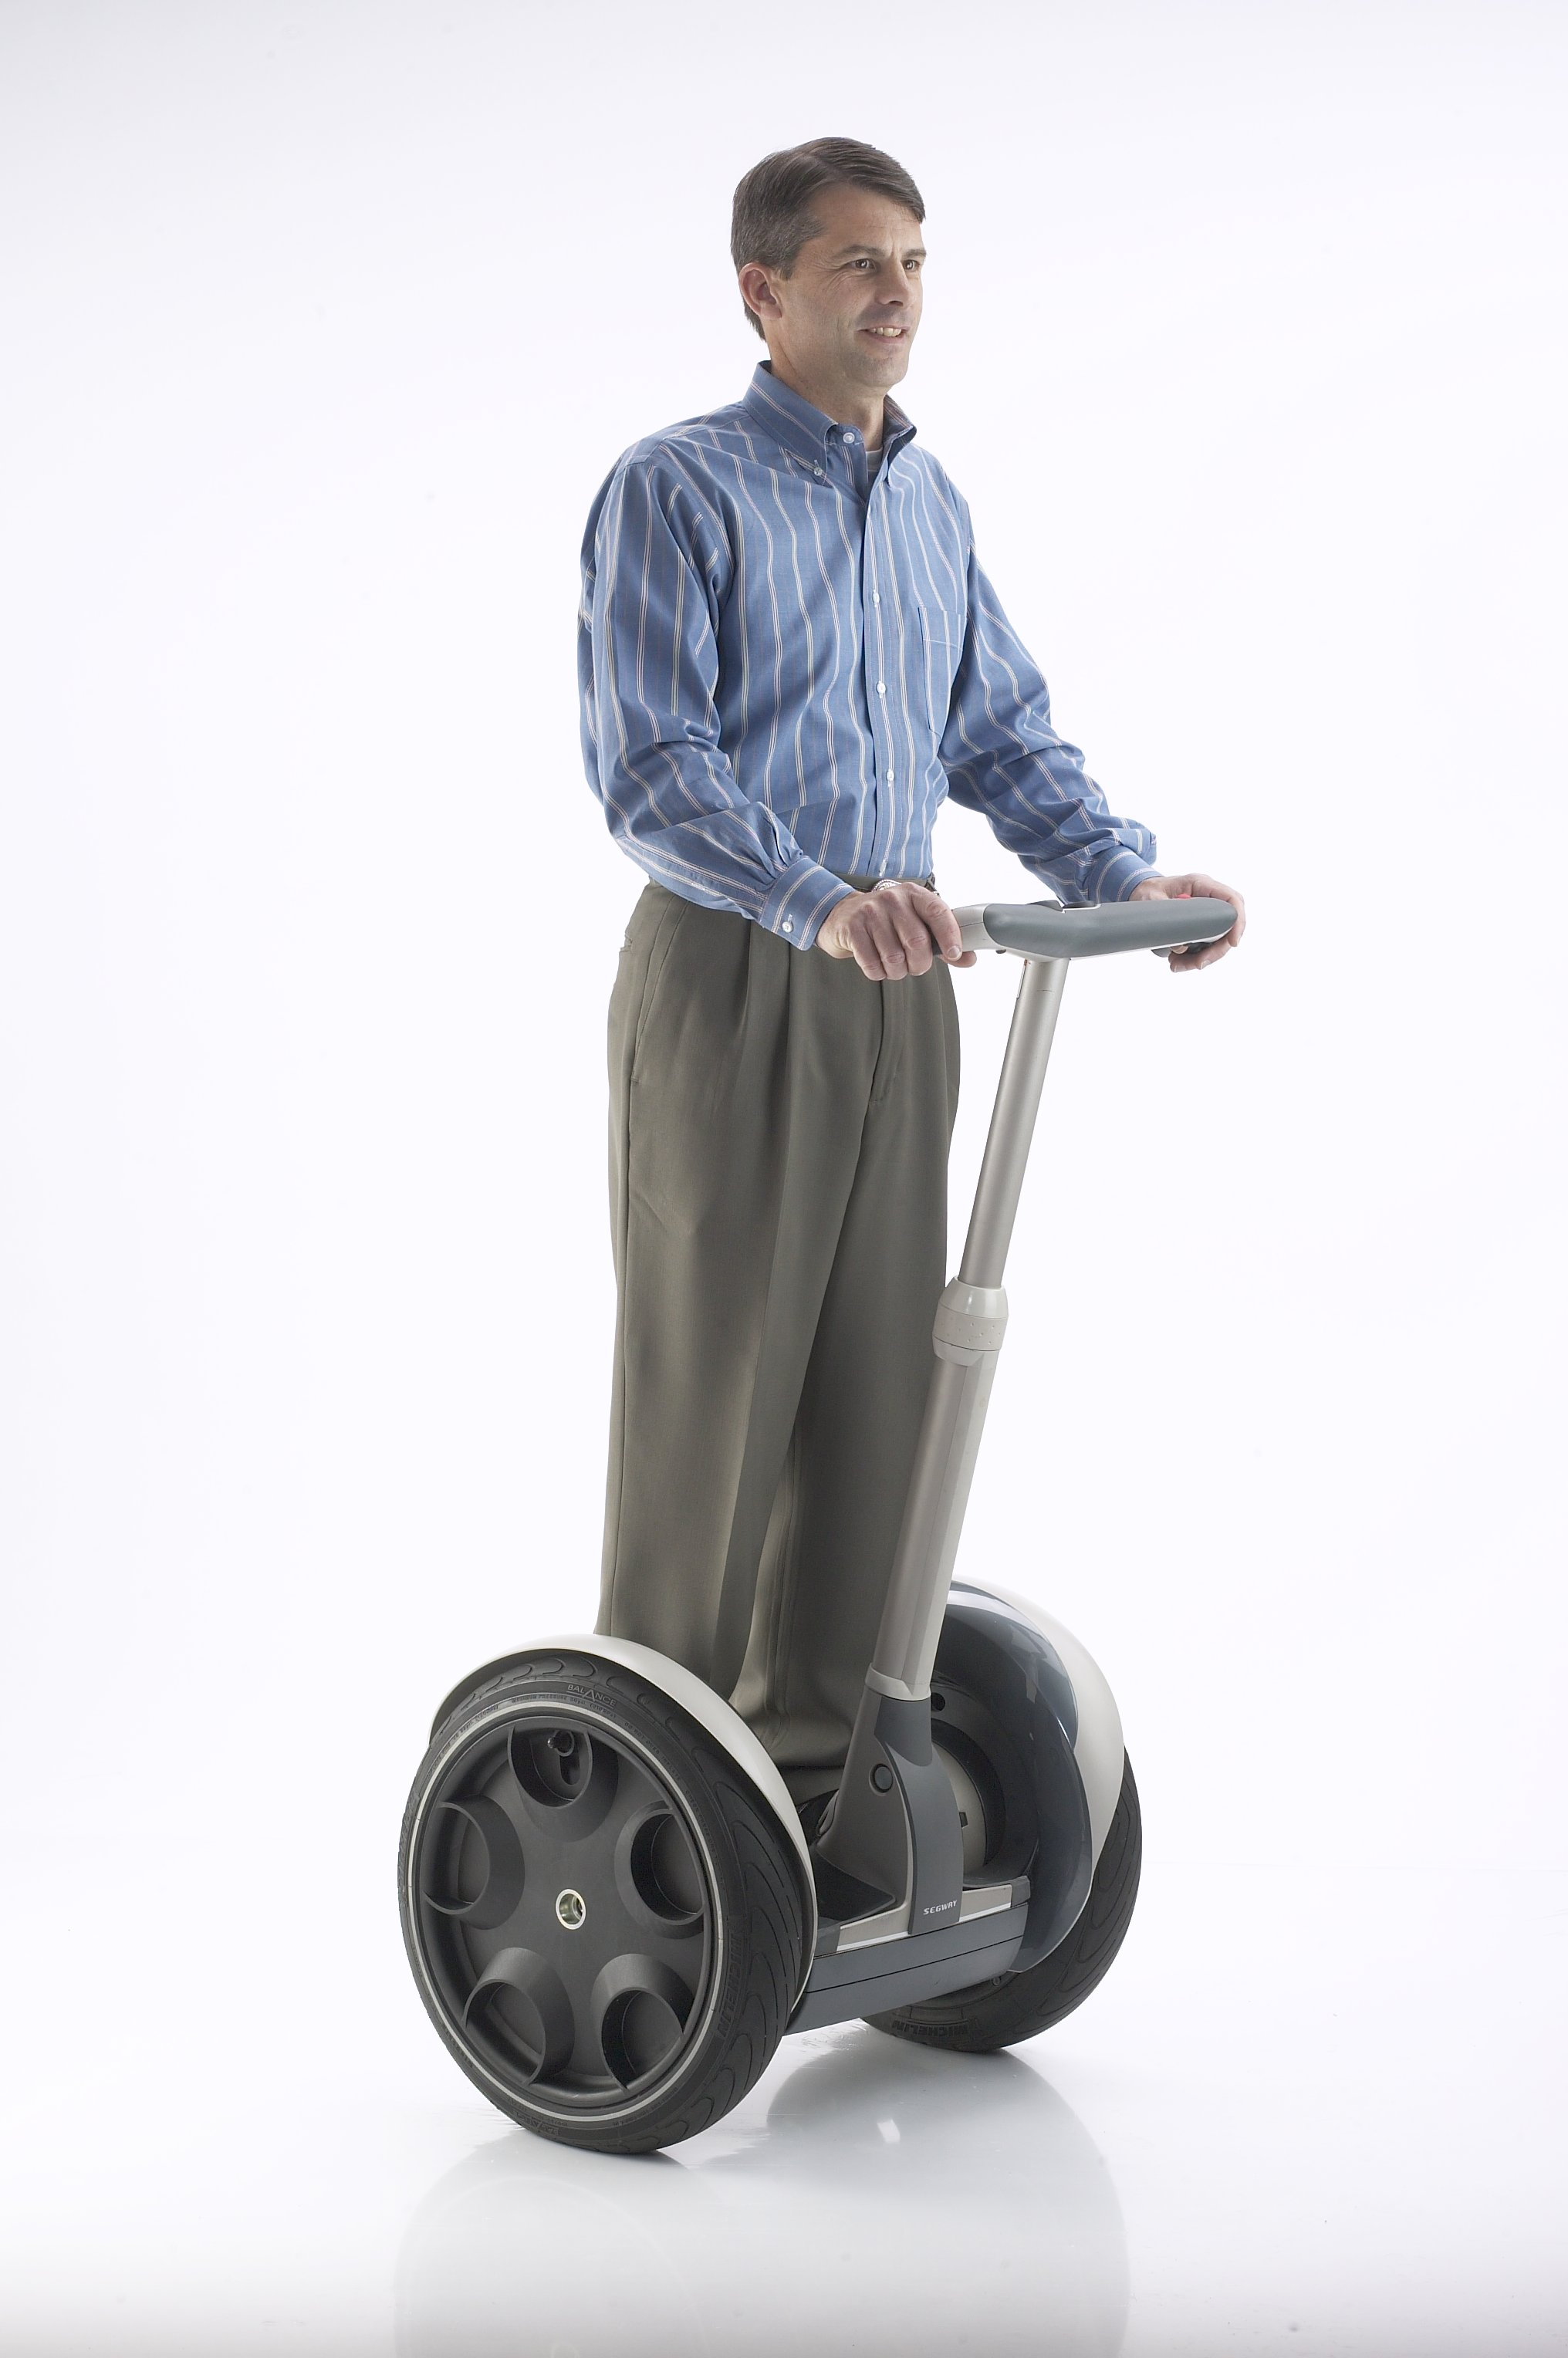
\includegraphics[width=0.3\textwidth]{man_on_wheels.jpg}
\end{figure}

\begin{abstract}
    We study the nonlinear, inherently unstable inverted pendulum. The goal is to maintain the
    pendulum angle $\theta(t) = 0$ by using a feedback controller with some sensors and an actuator to produce an
    input force $f(t)$. The cart has mass $m_1$, the pendulum point has mass $m_2$, and we assume that the pendulum
    rod is massless. There are two possible outputs, the pendulum angle $\theta(t)$ and the cart displacement $w(t)$.
\end{abstract}

\newpage

\tableofcontents

\newpage

\pagenumbering{arabic}

\section{State-space representation, linearization, and simulation}

\subsection{Non-linear state space realization}

The nonlinear equations of motion for the inverted pendulum balance system is given by
\begin{align}
    -m_2 L \Ddot{w} \cos\theta + m_2 L^2 \Ddot{\theta} - m_2 g L \sin\theta &= 0\\
    (m_1 + m_2) \Ddot{w} - m_2 L \Ddot{\theta} \cos\theta + m_2 L \dot{\theta}^2 \sin\theta &= f(t)
\end{align}
% \begin{equation}
%     -\Ddot{w} \cos\theta + L \Ddot{\theta} - g\sin\theta = 0
% \end{equation}
Due to equations of motion being second order in time derivatives, we chose the following variables as state variables
\begin{equation}
    x = 
    \begin{bmatrix}
        x_1\\
        x_2\\
        x_3\\
        x_4
    \end{bmatrix}
    =
    \begin{bmatrix}
        \theta\\
        \dot{\theta}\\
        w\\
        \dot{w}
    \end{bmatrix}
\end{equation}
We can solve for the second time derivatives in terms of lower order derivatives
\begin{align}
    (m_1 + m_2) L \Ddot{\theta} - m_2 L \Ddot{\theta} \cos^2\theta - (m_1 + m_2) g \sin\theta + m_2 L \dot{\theta}^2 \sin\theta \cos\theta &= f(t) \cos\theta\\
    (m_1 + m_2 \sin^2\theta) L \Ddot{\theta} - (m_1 + m_2) g \sin\theta + \frac{1}{2} m_2 L \dot{\theta}^2 \sin2\theta &= f(t) \cos\theta
\end{align}

\begin{align}
    (m_1 + m_2) \Ddot{w} - m_2  \Ddot{w} \cos^2\theta + m_2 L \dot{\theta}^2 \sin\theta - m_2 g \sin\theta \cos\theta &= f(t)\\
    (m_1 + m_2 \sin^2\theta) \Ddot{w} + m_2 L \dot{\theta}^2 \sin\theta - \frac{1}{2} m_2 g \sin2\theta &= f(t)
\end{align}
In terms of the state variables, the non-linear state space equation is given by
\begin{equation}
    \dot{x}
    =
    \begin{bmatrix}
        \dot{x}_1\\
        \dot{x}_2\\
        \dot{x}_3\\
        \dot{x}_4
    \end{bmatrix}
    =
    \begin{bmatrix}
        x_2\\
        \frac{g}{L} \frac{m_1 + m_2}{m_1 + m_2 \sin^2 x_1} \sin x_1 - \frac{1}{2} \frac{m_2}{m_1 + m_2 \sin^2 x_1} \sin(2x_1) {x_2}^2\\
        x_4\\
        -L\frac{m_2}{m_1 + m_2 \sin^2 x_1} \sin x_1 {x_2}^2 + \frac{g}{2} \frac{m_2}{m_1 + m_2 \sin^2 x_1} \sin(2 x_1)
    \end{bmatrix}
    +
    \begin{bmatrix}
        0\\
        \frac{1}{L} \frac{\cos x_1}{m_1 + m_2 \sin^2 x_1}\\
        0\\
        \frac{1}{m_1 + m_2 \sin^2 x_1}
    \end{bmatrix}
    u(t)
\end{equation}
The output vector is $y = \left[\theta \ w \right]^T = \left[x_1 \ x_3 \right]^T$
\begin{equation}
    y
    =
    \begin{bmatrix}
        x_1\\
        x_2
    \end{bmatrix}
    =
    \begin{bmatrix}
        1 & 0 & 0 & 0\\
        0 & 0 & 1 & 0
    \end{bmatrix}
    \begin{bmatrix}
        x_1\\
        x_2\\
        x_3\\
        x_4
    \end{bmatrix}
\end{equation}

\subsection{Linearization around equilibrium}

The equilibrium points are given by solving for vanishing time derivatives, i.e. $\dot{x} = 0$
\begin{equation}
    - m_2 g L \sin x_1 = 0
\end{equation}
Which has two solutions corresponding to pendulum up and down positions
\begin{equation}
    x_1^u = 0,\ x_1^d = \pi 
\end{equation}
Linearizing the system around $x_1^u$
\begin{equation}
    \sin x_1 = x_1,\ \cos x_1 = 1 
\end{equation}
The state space model is given by
\begin{align}
    \dot{x}
    =
    \begin{bmatrix}
        \dot{x}_1\\
        \dot{x}_2\\
        \dot{x}_3\\
        \dot{x}_4
    \end{bmatrix}
    &=
    \begin{bmatrix}
        0 & 1 & 0 & 0\\
        \frac{g}{L} \frac{m_1 + m_2}{m_1} & 0 & 0 & 0\\
        0 & 0 & 0 & 1\\
        g \frac{m_2}{m_1} & 0 & 0 & 0
    \end{bmatrix}
    \begin{bmatrix}
        x_1\\
        x_2\\
        x_3\\
        x_4
    \end{bmatrix}
    +
    \begin{bmatrix}
        0\\
        \frac{1}{L m_1}\\
        0\\
        \frac{1}{m_1}
    \end{bmatrix}
    u(t)\\
    y
    &=
    \begin{bmatrix}
        x_1\\
        x_3
    \end{bmatrix}
    =
    \begin{bmatrix}
        1 & 0 & 0 & 0\\
        0 & 0 & 1 & 0
    \end{bmatrix}
    \begin{bmatrix}
        x_1\\
        x_2\\
        x_3\\
        x_4
    \end{bmatrix}
\end{align}
Linearizing the system around $x_1^d = \pi$
\begin{equation}
    \sin x_1 = - x_1,\ \cos x_1 = -1
\end{equation}
The state space model is given by
\begin{align}
    \dot{x}
    =
    \begin{bmatrix}
        \dot{x}_1\\
        \dot{x}_2\\
        \dot{x}_3\\
        \dot{x}_4
    \end{bmatrix}
    &=
    \begin{bmatrix}
        0 & 1 & 0 & 0\\
        -\frac{g}{L} \frac{m_1 + m_2}{m_1} & 0 & 0 & 0\\
        0 & 0 & 0 & 1\\
        g \frac{m_2}{m_1} & 0 & 0 & 0
    \end{bmatrix}
    \begin{bmatrix}
        x_1\\
        x_2\\
        x_3\\
        x_4
    \end{bmatrix}
    +
    \begin{bmatrix}
        0\\
        -\frac{1}{L m_1}\\
        0\\
        \frac{1}{m_1}
    \end{bmatrix}
    u(t)\\
    y
    &=
    \begin{bmatrix}
        x_1\\
        x_3
    \end{bmatrix}
    =
    \begin{bmatrix}
        1 & 0 & 0 & 0\\
        0 & 0 & 1 & 0
    \end{bmatrix}
    \begin{bmatrix}
        x_1\\
        x_2\\
        x_3\\
        x_4
    \end{bmatrix}
\end{align}
Hereafter, we will focus on the state space model for the state space model constructed from the linearization about the pendulum up state.

\subsection{State-space model simulations with no input}
\label{sec:sim-no-input}
We simulate the cart position and pendulum position for the initial conditions $\theta_0 = 0$, $w_0 = 0$, with vanishing input $u(t) = 0$ with parameters $m_1 = 2$kg, $m_2 = 1$kg, $L = 0.75$m, $g = 10$m/s${}^2$, for $t \in [0,1.5]$s. The results are given in Figures \ref{fig:1}, \ref{fig:2}. MATLAB source is provided in Appendix \ref{app:zero-input-sim}. By increasing the simulation time, we can see that while the non-linear state simulation is stable, the linear state simulation is unstable.

\subsection{State-space model simulations with step input}
We simulate the cart position and pendulum position for the same initial conditions and parameters as Sec \ref{sec:sim-no-input}, but with a step function input \ref{fig:3}, \ref{fig:4}. MATLAB source is provided in Appendix. From the simulations we see now the nonlinear simulation results are also unstable \ref{fig:5}. 

\section{Controllability analysis}

\subsection{Controllability matrix}

By using the MATLAB Symbolic Toolbox \ref{app:controllability}, we calculate the controllability matrix
\begin{equation}
    \cC = \left[B | AB | A^2B | A^3B\right]
    =
    \begin{bmatrix}
    0 & 1/L m_1 & 0 & g (m_1 + m_2)/L^2 {m_1}^2\\
    1/L m_1 & 0 & g (m_1 + m_2)/L^2 {m_1}^2 & 0\\
    0 & 1/m_1 & 0 & g m_2/L {m_1}^2\\
    1/m_1 & 0 &  g m_2/L{m_1}^2 & 0
    \end{bmatrix}
\end{equation}
It has determinant
\begin{equation}
    \det\cC = \frac{g^2}{4 {m_1}^2} \neq 0
\end{equation}
Since the determinant is non-zero, all the rows and columns are linearly independent, therefore the controllability matrix has full rank. Given that $g$ can never be zero, and the mass of the cart $m_1$ is non vanishing, the system is controllable for all values of the parameters $g,L,m_1,m_2$.

\subsection{Driving to arbitrary stationary states}

The fact that the system is controllable implies that we can drive the system from any initial state to any desired final state in finite time using the appropriate application of the force $f(t)$. Most importantly, we can drive any arbitrary initial stationary state to the another stationary state of pendulum up.

\subsection{Controllable canonical form}
\label{sec:ccf}
The operator $T$ that transforms a controllable system to controllable canonincal form is given by
\begin{equation}
    T
    =
    \begin{bmatrix}
        q\\
        q \cC\\
        \vdots\\
        q \cC^{n-1}
    \end{bmatrix}
\end{equation}
where $q$ is the last row of the inverse of the controllability matrix, $\cC^{-1}$. For the inverted pendulum balance system, it is given by
\begin{equation}
    q = \left[0.1125\ 0.0000 -0.1500\ 0.0000\right]
\end{equation}
and the transformation matrix is given by
\begin{equation}
    T
    =
    \begin{bmatrix}
        0.1125 & 0 & -0.1500 & 0\\
        0 & 0.1125 & 0 & -1.500\\
        1.500 & 0 & 0 & 0\\
        0 & 1.500 & 0 & 0
    \end{bmatrix}
\end{equation}
Under a linear transformation of the state space variables to new state varaibles under $z_\text{ccf} = T x$, the matrix coefficients transform as
\begin{align}
    A_\text{ccf} &= TAT^{-1}\\
    B_\text{ccf} &= TB\\
    C_\text{ccf} &= CT^{-1}\\
    D_\text{ccf} &= D
\end{align}
The controllable canonical form is given by
\begin{align}
        x
    &=
    \begin{bmatrix}
        0 & 1 & 0 & 0\\
        0 & 0 & 1 & 0\\
        0 & 0 & 0 & 1\\
        0 & 0 & 20 & 0
    \end{bmatrix}
    \begin{bmatrix}
        x_1\\
        x_2\\
        x_3\\
        x_4
    \end{bmatrix}
    +
    \begin{bmatrix}
        0\\
        0\\
        0\\
        1
    \end{bmatrix}
    u(t)\\
    y
    &=
    \begin{bmatrix}
        0 & 0 & 0.667 & 0
    \end{bmatrix}
    \begin{bmatrix}
        x_1\\
        x_2\\
        x_3\\
        x_4
    \end{bmatrix}
\end{align}

\subsection{Diagonal canonical form}

The determinant of the $A$ matrix is zero. Therefore it is not invertible. Hence a diagonal canonical form representation of the state system is not possible.

\section{Observability analysis}

\subsection{Observability of different sensors}

The observability matrix is given by
\begin{equation}
    \cO
    =
    \begin{bmatrix}
        C\\
        C A\\
        C A^2\\
        C A^3
    \end{bmatrix}
\end{equation}

If the only output is the pendulum angle $y = \theta$ then the state to output matrix is given by
$C =
\begin{bmatrix}
    1 & 0 & 0 & 0
\end{bmatrix}$. Therefore the observability matrix is given by
\begin{equation}
    \cO_{\theta}
    =
    \begin{bmatrix}
        1 & 0 & 0 & 0\\
        0 & 1 & 0 & 0\\
        g (m_1 + m_2) / L m_1 & 0 & 0 & 0\\
        0 & g (m_1 + m_2) / L m_1 & 0 & 0
    \end{bmatrix}
\end{equation}
Since $\text{rank}\ \cO_\theta = 2 \neq 4$, the observability matrix is not full rank. Therefore the system is not observable when there is only a single output $\theta$.

If the only output is the cart position $y = w$ then the state to output matrix is given by
$C =
\begin{bmatrix}
    0 & 0 & 1 & 0
\end{bmatrix}$. Therefore the observability matrix is given by
\begin{equation}
    \cO_{\theta}
    =
    \begin{bmatrix}
        0 & 0 & 1 & 0\\
        0 & 0 & 0 & 1\\
        g m_2 / m_1 & 0 & 0 & 0\\
        0 & g m_2 / m_1 & 0 & 0
    \end{bmatrix}
\end{equation}
Since $\text{rank}\ \cO_w = 4$, the observability matrix is full rank. Therefore the system is observable when there is a single output $w$.

If the output is the pendulum angle and the cart position $y = [\theta\ w]^T$ then the state to output matrix is given by
$C =
\begin{bmatrix}
    1 & 0 & 0 & 0\\
    0 & 0 & 1 & 0
\end{bmatrix}$. Therefore the observability matrix is given by
\begin{equation}
    \cO_{\theta w}
    =
    \begin{bmatrix}
        1 & 0 & 0 & 0\\
        0 & 0 & 1 & 0\\
        0 & 1 & 0 & 0\\
        0 & 0 & 0 & 1\\
        g (m_1 + m_2) / L m_1 & 0 & 0 & 0\\
        g m_2 / m_1 & 0 & 0 & 0\\
        0 & g (m_1 + m_2) / L m_1 & 0 & 0\\
        0 & g m_2 / m_1 & 0 & 0
    \end{bmatrix}
\end{equation}
Since $\text{rank}\ \cO_{\theta w} = 4$, the observability matrix is full rank. Therefore the system is observable when we observe both the cart position and pendulum angle.

\subsection{Observable canonical form}
\label{sec:ocf}
The transfer function of the system for the specified parameters is given by
\begin{equation}
    G(s) = \frac{0.667 s^2}{s^4 - 20 s^2}
\end{equation}
By using the coefficients in the denominator and the numerator
\begin{equation}
    \alpha
    =
    \begin{bmatrix}
        0 & 0 & -20 & 0 
    \end{bmatrix}
    ,\ 
    \beta
    =
    \begin{bmatrix}
        0 & 0 & 0.667 & 0 
    \end{bmatrix}
\end{equation}
we can construct the observable canonical form, given by
\begin{align}
        x
    &=
    \begin{bmatrix}
        0 & 0 & 0 & 0\\
        1 & 0 & 0 & 0\\
        0 & 1 & 0 & 20\\
        0 & 0 & 1 & 0
    \end{bmatrix}
    \begin{bmatrix}
        x_1\\
        x_2\\
        x_3\\
        x_4
    \end{bmatrix}
    +
    \begin{bmatrix}
        0\\
        0\\
        0.667\\
        0
    \end{bmatrix}
    u(t)\\
    y
    &=
    \begin{bmatrix}
        0 & 0 & 0 & 1
    \end{bmatrix}
    \begin{bmatrix}
        x_1\\
        x_2\\
        x_3\\
        x_4
    \end{bmatrix}
\end{align}

\subsection{CCF and OCF duality transformation}
We can see that the observable canonical form found in \ref{sec:ocf} is related to the controllable canonical form found in \ref{sec:ccf} by a duality transformation given by
\begin{align}
    A_\text{ocf} &= A_\text{ccf}^T\\
    B_\text{ocf} &= C_\text{ccf}^T\\
    C_\text{ocf} &= B_\text{ccf}^T\\
    D_\text{ocf} &= D_\text{ccf}
\end{align}

\section{Stability analysis}

Consider the Lyapunov function
\begin{equation}
    V(x) = x^T P x
\end{equation}
For zero input system, it's time derivative is given by
\begin{equation}
    \dot{V} = \dot{x}^T P x + x^T P \dot{x} = x^T (A^T P + P A) x
\end{equation}
Hence if we can find a $P$ such that
\begin{equation}
    A^T P + P A = - Q
\end{equation}
where $Q$ is a positive definite matrix, than the system is stable in the sense of Lyapunov, since the Lyapunov function would be monotonically decreasing in time.

For the parameters that we are working with, $A^T P + P A$ is given by
\begin{equation}
    \begin{bmatrix}
        40 p_{12} + 10 p_{14} & p_{11} + 20 p_{22} + 5 p_{24} & 20 p_{23} + 5 p_{34} & p_{13} + 20 p_{24} + 5 p_{44}\\
        p11 + 20 p_{22} + 5 p_{24} & 2 p_{12} & p_{13} & p_{14} + p_{23}\\
        20 p_{23} + 5 p_{34} & p_{13} & 0 & p_{33}\\
        p_{13} + 20 p_{24} + 5 p_{44} & p_{14} + p_{23} & p_{33} & 2 p_{34}
    \end{bmatrix}
\end{equation}
Due to the 0 in the diagonal, this matrix can never be equal to $-Q$. Therefore Lyapunov stability fails.

Resorting to eigenvalue analysis for stability we obtain
\begin{equation}
    \lambda 
    =
    \begin{bmatrix}
        0 & 0 & 4.4721  & - 4.4721
    \end{bmatrix}
\end{equation}
Since the system has a positive real eigenvalue, the system system is not stable.

\subsection{BIBO stability}

For the same system parameters, the system is also not BIBO stable due to the presence of eigenvalues that have positive real parts.

\section{State-feedback control design}

We consider a state-feedback control law with a step impulse reference input
\begin{equation}
    u = - K x + k_g r(t)
\end{equation}

We have the design specifications of 2 percent overshoot and 2s settling time. For a 2nd order system, the design specifications are related to the characteristic equation coefficients as follows
\begin{equation}
    \lambda(s) = s^2 + 2 \zeta \omega_0 s + \omega_0^2
\end{equation}

The overshoot and settling time are given by
\begin{align}
    M_p &= e^{-\pi \zeta / \sqrt{1 - \zeta^2}}\\
    T_s &\approx 4 / \zeta \omega_ 0
\end{align}
These design specifications give us the poles $-2.0000+i1.6061$ and $-2.0000-i1.6061$. Placing the other two poles 10 times further, the desired pole placement is given by
\begin{equation}
    p = 
    \begin{bmatrix}
        -2.0000+i1.6061 & -2.0000-i1.6061 & -20 & -21
    \end{bmatrix}
\end{equation}
The matrix $K$ that achieves this pole placement is given by
\begin{equation}
    K = 
    \begin{bmatrix}
        1.2268 & 0.2868 & -0.4145 & -0.2925
    \end{bmatrix}
    10e+3
\end{equation}
For a steady state response at the pendulum up position and an arbitrary cart position $y(\infty) = [0, 0,5]^T$, the reference gain is given by
\begin{equation}
    k_g = -207.2583
\end{equation}
The MATLAB calculations for pole placement for system respons design is given in Appendix \ref{app:state-feedback}, and the simulation results for different initial pendulum positions are given in Figures \ref{fig:6}, \ref{fig:7}, \ref{fig:8}.

\section{Observer and observer based control design}

In general we don't have access to the whole state space due to real world constraints. In those circumstances, we use observer based control.Creating a guess state $\hat{x}$, we design its asymptotic behaviour such that it matches the state-feedback results at late times. The dynamics of the guess state is given by
\begin{align}
    \dot{\hat{x}} &= A \hat{x} + B u + L (y - C \hat{x})\\
    \hat{y} &= C\hat{x}\\
    u &= -K\hat{x} + k_g r(t)
\end{align}
The error dynamics is given by
\begin{equation}
    \dot{e} = \frac{d}{dt}(\hat{x}-x) = (A-LC)e
\end{equation}
Therefore we aim to place the eigenvalues of $A-LC$ as far as possible in the left half plane such that the error asymptotes to 0, so that we can capture the state dynamics using our initial guess. For an observable system, we can design the observer gain matrix $L$ in such a way that we can arbitrarily chose the poles for error dynamics.

We use the same state gain matrix $K$ as in the previous section, and we design $L$ such that the eigenvalues of $A-LC$ is placed 10 times farther then the eigenvalues of $A-BK$. The observable systems are when there is a single output $y = [0,0,1,0]x$
\begin{equation}
    L = 1.0e+04 *[0.6592;3.7506;0.0085;0.2561]
\end{equation}
and when there is two outputs $y=[1,0,0,0;0,0,1,0]$
\begin{equation}
    L =[43.0132,3.3544;396.6016,111.0360;-1.1031,41.9868;-21.0492,354.2913]
\end{equation}
The MATLAB calculations are provided in Appendix \ref{app:observer_control}, and the simulation results are given in Figures \ref{fig:observer_sim_first} through \ref{fig:observer_sim_last}.

\section{Linear quadratic optimal control}

The cost function for linear quadratic control is given by
\begin{equation}
    J = \frac{1}{2}\int_{0}^{\infty}dt\left[x^T Q x + u^T R u\right]
\end{equation}
Choosing $Q = C^T C$, the cost function minimized output because
\begin{equation}
    J = \frac{1}{2}\int_{0}^{\infty}dt\left[x^T C^T C x + u^T R u\right] = \frac{1}{2}\int_{0}^{\infty}dt\left[y^T y + u^T R u\right]   
\end{equation}
Which is minimized by the state feedback $u = - K x$ with state feedback gain matrix given by
\begin{equation}
    K = R^{-1} B^T P
\end{equation}
where $P$ is the solution to the algebraic Ricatti equation
\begin{equation}
    A^T P + P A - P B R^{-1} B^T P + Q = 0
\end{equation}
For the output
\begin{equation}
    y =
    \begin{bmatrix}
        1 & 0 & 0 & 0\\
        0 & 0 & 1 & 0
    \end{bmatrix}
    x
\end{equation}
the optimal state feedback matrix is given by
\begin{equation}
    K = [72.2618,   16.8275,   -1.0000,   -2.9073]
\end{equation}
For the output
\begin{equation}
    y =
    \begin{bmatrix}
        100 & 0 & 0 & 0\\
        0 & 0 & 10 & 0
    \end{bmatrix}
    x
\end{equation}
the optimal state feedback matrix is given by
\begin{equation}
    K = [172.2427,   34.8813,  -10.0000,  -16.8667]
\end{equation}
The LQR optimization in MATLAB is provided in Appendix \ref{app:lqr}, and the simulation results for the state variables and optimal input are given in Figures \ref{fig:lqr1}, \ref{fig:lqr2}, \ref{fig:lqr3}, \ref{fig:lqr4} .

There is a considerable differences between the state responses for different output matrices, because when we use the second choice for the state to output matrix, a higher weight is put on the state variable $x_1$ compared to the state variable $x_3$. Therefore the LQR results exhibit a faster convergence rate.

\section{Robust control}
In real life applications, one must also consider arbitrary perturbations to system parameters in real time. For example, the mass of the pendulum could increase under the addition of external weight. The mass of the cart can decrease if it is fuel propelled. If we simply consider parameter variations while keeping the LQR state feedback gain matrix fixed, we lose stability after the perturbation exceeds a certain threshold. We can demonstrate this by adding extra mass to the pendulum in real time. The results are provided in Figures \ref{fig:lqr_perturb_5kg} and \ref{fig:lqr_perturb_1kg}.

I have tested whether the LQR control law we have is robust in this sense by increasing m2 by 5kg, at $t = 20$s. I simply changed the mass parameter after the first-time evolution loop and ran another loop without changing the optimal state feedback gain. We could simply rerun the LQR algorithm to find the optimal K, but I don't think this would be feasible in real life. Is there a clever way to achieve robustness against parameter variations in real time when the instance at which the perturbation is performed is unknown?

On another note, it's also interesting to understand what is the range of parameter perturbations that LQR can tolerate. For example, if the mass is perturbed by 1kg, the system still achieves the desired steady state response.

To achieve robust LQR, we consider nonlinear terms in the cost function
\begin{equation}
    J = \frac{1}{2} \int_{0}^{\infty}dt \left[x^T Q x + u^T R u + \text{nonlinear terms} \dots \right]
\end{equation}
Non-linear corrections, linear region constraints?

\section{Adaptive control}


\newpage
\appendix

\section{State-space representation simulations}
\label{app:zero-input-sim}

\begin{verbatim}
clear all;

m1 = 2;
m2 = 1;
g = 10;
L = 0.75;

A = [0 1 0 0;g*(m1+m2)/(m1*L) 0 0 0;0 0 0 1;g*m2/m1 0 0 0];
B = [0;-1/(L*m1);0;1/m1];
C = [1 0 0 0; 0 0 1 0];
eig(A)
cm = ctrb(A,B);
rank(cm)
om = obsv(A,C);
rank(om)

x(:,1) = [0.1; 0; 0; 0];
y(:,1) = C*x(:,1);
X(:,1) = x(:,1);
Y(:,1) = C*X(:,1);
t = 0:0.01:1.5; %0.01 time span of interest
nt = length(t); % number of time steps
dt = t(2) - t(1);

% case 1: linear
for i = 1:nt-1
u(i) = 1;
x_dot(:,i) = A*x(:,i) + B*u(i);
x(:,i+1) = x(:,i) + x_dot(:,i)*dt;
y(:,i+1) = C*x(:,i+1);
end

% case 2: non-linear
for i =1:nt-1
u(i) = 1;
X_dot(1,i) = X(2,i);
X_dot(2,i) = (g*(m1+m2)/L)*sin(X(1,i))/(m1+m2*sin(X(1,i))^2)
           - 0.5*m2*sin(2*X(1,i))*X(2,i)^2/(m1+m2*sin(X(1,i))^2)
           + u(i)*(1/L)*cos(X(1,i))/(m1+m2*sin(X(1,i))^2);
X_dot(3,i) = X(4,i);
X_dot(4,i) = -L*m2*sin(X(1,i))*X(2,i)^2/(m1+m2*sin(X(1,i))^2)
           + 0.5*g*m2*sin(2*X(1,i))/(m1+m2*sin(X(1,i))^2)
           + u(i)/(m1+m2*sin(X(1,i))^2);
X(:,i+1) = X(:,i) + X_dot(:,i)*dt;
Y(:,i+1) = C*X(:,i+1);
end

figure
plot(t,Y(1,:),'b',t,y(1,:),'r','linewidth',2)
set(gca,'fontsize',18)
legend({'nonlinear','linear'},'Interpreter', 'latex')
title('pendulum angle')
legend boxoff
xlabel('Time (s)')
ylabel('Angle (rad)')
print(gcf,'theta_open_loop.png','-dpng','-r300');

figure
plot(t,Y(2,:),'b',t,y(2,:),'r','linewidth',2)
set(gca,'fontsize',18)
legend({'nonlinear','linear'},'Interpreter', 'latex')
title('cart position')
legend boxoff
xlabel('Time (s)')
ylabel('Position (m)')
print(gcf,'w_open_loop.png','-dpng','-r300');
\end{verbatim}

\section{Controllability calculations}

\subsection{Proof of controllability}
\label{app:controllability}

    \begin{verbatim}
clear;clc

syms g L m1 m2;

% ss model
A = [0 1 0 0;g/L*(m1+m2)/m1 0 0 0;0 0 0 1;g*m2/m1 0 0 0];
B = [0;1/(L*m1);0;1/m1];
C = [1 0 0 0];
D = 0;

% controllability matrix
cc = [B A*B A^2*B A^3*B]

% determinant
det(cc)
\end{verbatim}

        \color{lightgray} \begin{verbatim} 
cc =
 
[       0, 1/(L*m1),                        0, (g*(m1 + m2))/(L^2*m1^2)]
[1/(L*m1),        0, (g*(m1 + m2))/(L^2*m1^2),                        0]
[       0,     1/m1,                        0,          (g*m2)/(L*m1^2)]
[    1/m1,        0,          (g*m2)/(L*m1^2),                        0]
 
 
ans =
 
g^2/(L^4*m1^4)
 
\end{verbatim} \color{black}

\subsection{Controllable canonical form}
\label{app:ccf}
    \begin{verbatim}
clear;clc

m1 = 2;
m2 = 1;
g = 10;
L = 0.75;

A = [0 1 0 0;g/L*(m1+m2)/m1 0 0 0;0 0 0 1;g*m2/m1 0 0 0];
B = [0;1/(L*m1);0;1/m1];
C = [1 0 0 0];
D = 0;

[E,V] = eig(A)

cntr = [B A*B A^2*B A^3*B]
icntr = inv(cntr)
q = icntr(4,:)
T = [q;q*A;q*A^2;q*A^3]
Ac = T*A*inv(T)
Bc = T*B
Cc = C*inv(T)
\end{verbatim}

        \color{lightgray} \begin{verbatim}
E =

         0         0    0.2117   -0.2117
         0         0    0.9468    0.9468
    1.0000   -1.0000    0.0529   -0.0529
         0    0.0000    0.2367    0.2367


V =

         0         0         0         0
         0         0         0         0
         0         0    4.4721         0
         0         0         0   -4.4721


cntr =

         0    0.6667         0   13.3333
    0.6667         0   13.3333         0
         0    0.5000         0    3.3333
    0.5000         0    3.3333         0


icntr =

         0   -0.7500         0    3.0000
   -0.7500         0    3.0000         0
         0    0.1125         0   -0.1500
    0.1125         0   -0.1500         0


q =

    0.1125         0   -0.1500         0


T =

    0.1125         0   -0.1500         0
         0    0.1125         0   -0.1500
    1.5000         0         0         0
         0    1.5000         0         0


Ac =

         0    1.0000         0   -0.0000
         0         0    1.0000         0
         0         0         0    1.0000
         0         0   20.0000         0


Bc =

         0
   -0.0000
         0
    1.0000


Cc =

         0         0    0.6667         0

\end{verbatim} \color{black}

\section{Observability calculations}

\subsection{Observability for different sensors}

    \begin{verbatim}
clear;clc

syms g L m1 m2;

% ss model
A = [0 1 0 0;g/L*(m1+m2)/m1 0 0 0;0 0 0 1;g*m2/m1 0 0 0];
B = [0;1/(L*m1);0;1/m1];

C_theta = [1 0 0 0];
C_w = [0 0 1 0];
C_theta_and_w = [1 0 0 0;0 0 1 0];

D = 0;

obsv_theta = [C_theta;C_theta*A;C_theta*A^2;C_theta*A^3]
rank(obsv_theta)

obsv_w = [C_w;C_w*A;C_w*A^2;C_w*A^3]
rank(obsv_w)

obsv_theta_and_w = [C_theta_and_w;C_theta_and_w*A;C_theta_and_w*A^2;C_theta_and_w*A^3]
rank(obsv_theta_and_w)
\end{verbatim}

        \color{lightgray} \begin{verbatim} 
obsv_theta =
 
[                   1,                    0, 0, 0]
[                   0,                    1, 0, 0]
[(g*(m1 + m2))/(L*m1),                    0, 0, 0]
[                   0, (g*(m1 + m2))/(L*m1), 0, 0]
 

ans =

     2

 
obsv_w =
 
[        0,         0, 1, 0]
[        0,         0, 0, 1]
[(g*m2)/m1,         0, 0, 0]
[        0, (g*m2)/m1, 0, 0]
 

ans =

     4

 
obsv_theta_and_w =
 
[                   1,                    0, 0, 0]
[                   0,                    0, 1, 0]
[                   0,                    1, 0, 0]
[                   0,                    0, 0, 1]
[(g*(m1 + m2))/(L*m1),                    0, 0, 0]
[           (g*m2)/m1,                    0, 0, 0]
[                   0, (g*(m1 + m2))/(L*m1), 0, 0]
[                   0,            (g*m2)/m1, 0, 0]
 

ans =

     4

\end{verbatim} \color{black}

\section{Stability calculations}

    \begin{verbatim}
clear;clc

syms p11 p12 p13 p14 p22 p23 p24 p33 p34 p44;
m1 = 2;
m2 = 1;
g = 10;
L = 0.75;

A = [0 1 0 0;g*(m1+m2)/(m1*L) 0 0 0;0 0 0 1;g*m2/m1 0 0 0];
P = [p11 p12 p13 p14;p12 p22 p23 p24;p13 p23 p33 p34;p14 p24 p34 p44]

Q = simplify(transpose(A)*P+P*A)

solve(Q == eye(4),[p11 p12 p13 p14 p22 p23 p24 p33 p34 p44])

eig(A)
\end{verbatim}

        \color{lightgray} \begin{verbatim} 
P =
 
[p11, p12, p13, p14]
[p12, p22, p23, p24]
[p13, p23, p33, p34]
[p14, p24, p34, p44]
 
 
Q =
 
[     40*p12 + 10*p14, p11 + 20*p22 + 5*p24, 20*p23 + 5*p34, p13 + 20*p24 + 5*p44]
[p11 + 20*p22 + 5*p24,                2*p12,            p13,            p14 + p23]
[      20*p23 + 5*p34,                  p13,              0,                  p33]
[p13 + 20*p24 + 5*p44,            p14 + p23,            p33,                2*p34]
 

ans = 

  struct with fields:

    p11: [0×1 sym]
    p12: [0×1 sym]
    p13: [0×1 sym]
    p14: [0×1 sym]
    p22: [0×1 sym]
    p23: [0×1 sym]
    p24: [0×1 sym]
    p33: [0×1 sym]
    p34: [0×1 sym]
    p44: [0×1 sym]


ans =

         0
         0
    4.4721
   -4.4721

\end{verbatim} \color{black}

\section{MATLAB state control}
\label{app:state-feedback}
\begin{verbatim}
clear all;

m1 = 2;
m2 = 1;
g = 10;
L = 0.75;

A = [0 1 0 0;g*(m1+m2)/(m1*L) 0 0 0;0 0 0 1;g*m2/m1 0 0 0];
B = [0;1/(L*m1);0;1/m1];
C = [1 0 0 0; 0 0 1 0];
eig(A)
cm = ctrb(A,B);
rank(cm)
om = obsv(A,C);
rank(om)

        \color{lightgray} \begin{verbatim}
ans =

         0
         0
    4.4721
   -4.4721


ans =

     4


ans =

     4

\color{black}
    
x(:,1) = [pi; 0; 0; 0];
y(:,1) = C*x(:,1);
t = 0:0.01:10; %0.01 time span of interest
nt = length(t); % number of time steps
dt = t(2) - t(1);
% reference input
for i = 1:nt
    r(:,i) = 1;
end

% case 1: open loop
for i = 1:nt-1
x_dot(:,i) = A*x(:,i);
x(:,i+1) = x(:,i) + x_dot(:,i)*dt;
y(:,i+1) = C*x(:,i+1);
end

% figure
% plot(t,y(1,:),'b',t,y(2,:),'r','linewidth',2)
% set(gca,'fontsize',18)
% legend({'$\theta$','$w$'},'Interpreter', 'latex')
% title('open loop')
% legend boxoff
% xlabel('Time (s)')

% case 2: state-feedback
Mp = 2; % percent overshoot
Ts = 2; % transient time
Mlog = log(Mp/100);
MlogSquared = Mlog^2;
zeta = sqrt(MlogSquared/(pi^2+MlogSquared));
w0 = 4/(Ts*zeta);
P = roots([1 2*zeta*w0 w0^2])
p1 = P(1);
p2 = P(2);
P = [p1 p2 -20 -21]
K = place(A,B,P)
A1 = A - B*K;
eig(A1)

yss = [0; 0.5]; % steady state response
kg = -C*inv(A-B*K)*B
kg = yss(2)/kg(2)

u(:,1) = -K*x(:,1) + kg*r(:,1);
for i = 1:nt-1
x_dot(:,i) = A*x(:,i) + B*u(:,i);
x(:,i+1) = x(:,i) + x_dot(:,i)*dt;
y(:,i+1) = C*x(:,i+1);
u(:,i+1) = -K*x(:,i+1) + kg*r(:,i+1);
end

% figure
% plot(t,r(1,1:nt),'k--',t,y(1,:),'b',t,y(2,:),'r','linewidth',2)
% set(gca,'fontsize',18)
% legend({'$r$','$\theta$','$w$'},'Interpreter', 'latex')
% title('state-feedback')
% legend boxoff
% xlabel('Time (s)')
% print(gcf,'state_feedback.png','-dpng','-r300');

        \color{lightgray}
P =

  -2.0000 + 1.6061i
  -2.0000 - 1.6061i


P =

  -2.0000 + 1.6061i  -2.0000 - 1.6061i -20.0000 + 0.0000i -21.0000 + 0.0000i


K =

   1.0e+03 *

    1.2268    0.2868   -0.4145   -0.2925


ans =

 -21.0000 + 0.0000i
 -20.0000 + 0.0000i
  -2.0000 + 1.6061i
  -2.0000 - 1.6061i

kg =

 -207.2583

\end{verbatim} \color{black}


\section{MATLAB observer control}
\label{app:observer_control}
\begin{verbatim}
clear all; clc
% define systems
m1 = 2;
m2 = 1;
g = 10;
L = 0.75;

A = [0 1 0 0;g*(m1+m2)/(m1*L) 0 0 0;0 0 0 1;g*m2/m1 0 0 0];
B = [0;1/(L*m1);0;1/m1];
C = [1 0 0 0; 0 0 1 0];
eig(A)
cm = ctrb(A,B);
rank(cm)
om = obsv(A,C);
rank (om)
% initialization
x(:,1) = [0.1;0;0;0];
y(:,1) = C*x(:,1);
x_hat(:,1) = [0;0;0;0];
y_hat(:,1) = C*x_hat(:,1);
t = 0:0.01:20; %0.01 time span of interest
nt = length(t); % number of time steps
dt = t(2) - t(1);
% reference input
for i = 1:nt
    r(:,i) = 1;
    u(:,i) = 1;
end

ans =

         0
         0
    4.4721
   -4.4721


ans =

     4


ans =

     4


p1 = -1; p2 = -2; p3 = -3; p4 = -4;
L = place(A',C',[p1 p2 p3 p4]);L = L';
L
A1 = A - L*C;
eig(A1)
for i = 1:nt-1
x_dot(:,i) = A*x(:,i)+B*u(:,i);
x(:,i+1) = x(:,i) + x_dot(:,i)*dt;
y(:,i+1) = C*x(:,i+1);
x_hat_dot(:,i) = A*x_hat(:,i) + B*u(:,i) + L*(y(:,i)- C*x_hat(:,i));
x_hat(:,i+1) = x_hat(:,i) + x_hat_dot(:,i)*dt;
y_hat(:,i+1) = C*x_hat(:,i+1);
end

figure
plot(t,x(1,:),'r',t,x_hat(1,:),'b-.','linewidth',2)
set(gca,'fontsize',18)
legend({'$x_1$','${\hat x}_1$'},'Interpreter', 'latex')
legend boxoff
title('open loop')
xlabel('Time (s)')
print(gcf,'fig1.png','-dpng','-r300');
figure
plot(t,x(2,:),'r',t,x_hat(2,:),'b-.','linewidth',2)
set(gca,'fontsize',18)
legend({'$x_2$','${\hat x}_2$'},'Interpreter', 'latex')
legend boxoff
title('open loop')
xlabel('Time (s)')
print(gcf,'fig2.png','-dpng','-r300');
figure
plot(t,x(3,:),'r',t,x_hat(3,:),'b-.','linewidth',2)
set(gca,'fontsize',18)
legend({'$x_3$','${\hat x}_3$'},'Interpreter', 'latex')
legend boxoff
title('open loop')
xlabel('Time (s)')
print(gcf,'fig3.png','-dpng','-r300');
figure
plot(t,x(4,:),'r',t,x_hat(4,:),'b-.','linewidth',2)
set(gca,'fontsize',18)
legend({'$x_4$','${\hat x}_4$'},'Interpreter', 'latex')
legend boxoff
title('open loop')
xlabel('Time (s)')
print(gcf,'fig4.png','-dpng','-r300');

L =

    5.9983   -0.0635
   27.9962   -0.1583
   -0.0520    4.0017
    4.8789    3.0038


ans =

   -4.0000
   -2.0000
   -1.0000
   -3.0000

Mp = 2; % percent overshoot
Ts = 2; % transient time
Mlog = log(Mp/100);
MlogSquared = Mlog^2;
zeta = sqrt(MlogSquared/(pi^2+MlogSquared));
w0 = 4/(Ts*zeta);
P = roots([1 2*zeta*w0 w0^2])
p1 = P(1);
p2 = P(2);
P = [p1 p2 -20 -21]
K = place(A,B,P)
A1 = A - B*K;
eig(A1)
% eigenvalues of(A - LC)
P2 = eig(A1)-[10;10;10;10];
L = place(A',C',P2);L = L';
L
A2 = A - L*C;
eig(A2)

u(:,1) = -K*x_hat(:,1);
for i = 1:nt-1
x_dot(:,i) = A*x(:,i)+ B*u(:,i);
x(:,i+1) = x(:,i) + x_dot(:,i)*dt;
y(:,i+1) = C*x(:,i+1);
x_hat_dot(:,i) = A*x_hat(:,i)+ B*u(:,i)+ L*(y(:,i)- C*x_hat(:,i));
x_hat(:,i+1) = x_hat(:,i) + x_hat_dot(:,i)*dt;
y_hat(:,i+1) = C*x_hat(:,i+1);
u(:,i+1) = -K*x_hat(:,i+1);
end

figure
plot(t,x(1,:),'r',t,x_hat(1,:),'b-.','linewidth',2)
set(gca,'fontsize',18)
legend({'$x_1$','${\hat x}_1$'},'Interpreter', 'latex')
legend boxoff
title('observer regulation control')
xlabel('Time (s)')
print(gcf,'fig5.png','-dpng','-r300');
figure
plot(t,x(2,:),'r',t,x_hat(2,:),'b-.','linewidth',2)
set(gca,'fontsize',18)
legend({'$x_2$','${\hat x}_2$'},'Interpreter', 'latex')
legend boxoff
title('observer regulation control')
xlabel('Time (s)')
print(gcf,'fig6.png','-dpng','-r300');
figure
plot(t,x(3,:),'r',t,x_hat(3,:),'b-.','linewidth',2)
set(gca,'fontsize',18)
legend({'$x_3$','${\hat x}_3$'},'Interpreter', 'latex')
legend boxoff
title('observer regulation control')
xlabel('Time (s)')
print(gcf,'fig7.png','-dpng','-r300');
figure
plot(t,x(4,:),'r',t,x_hat(4,:),'b-.','linewidth',2)
set(gca,'fontsize',18)
legend({'$x_4$','${\hat x}_4$'},'Interpreter', 'latex')
legend boxoff
title('observer regulation control')
xlabel('Time (s)')
print(gcf,'fig8.png','-dpng','-r300');

P =

  -2.0000 + 1.6061i
  -2.0000 - 1.6061i


P =

  -2.0000 + 1.6061i  -2.0000 - 1.6061i -20.0000 + 0.0000i -21.0000 + 0.0000i


K =

   1.0e+03 *

    1.2268    0.2868   -0.4145   -0.2925


ans =

 -21.0000 + 0.0000i
 -20.0000 + 0.0000i
  -2.0000 + 1.6061i
  -2.0000 - 1.6061i


L =

   43.0132    3.3544
  396.6016  111.0360
   -1.1031   41.9868
  -21.0492  354.2913


ans =

 -12.0000 + 1.6061i
 -12.0000 - 1.6061i
 -31.0000 + 0.0000i
 -30.0000 + 0.0000i

Mp = 2; % percent overshoot
Ts = 2; % transient time
Mlog = log(Mp/100);
MlogSquared = Mlog^2;
zeta = sqrt(MlogSquared/(pi^2+MlogSquared));
w0 = 4/(Ts*zeta);
P = roots([1 2*zeta*w0 w0^2])
p1 = P(1);
p2 = P(2);
P = [p1 p2 -20 -21]
K = place(A,B,P)
A1 = A - B*K;
eig(A1)
% eigenvalues of(A - LC)
P2 = eig(A1)-[10;10;10;10];
L = place(A',C',P2);L = L';
L
A2 = A - L*C;
eig(A2)

yss = [0; 0.5]; % steady state response
kg = -C*inv(A-B*K)*B
kg = yss(2)/kg(2)

u(:,1) = -K*x_hat(:,1) + kg*r(:,1);
for i = 1:nt-1
x_dot(:,i) = A*x(:,i)+ B*u(:,i);
x(:,i+1) = x(:,i) + x_dot(:,i)*dt;
y(:,i+1) = C*x(:,i+1);
x_hat_dot(:,i) = A*x_hat(:,i)+ B*u(:,i)+ L*(y(:,i)- C*x_hat(:,i));
x_hat(:,i+1) = x_hat(:,i) + x_hat_dot(:,i)*dt;
y_hat(:,i+1) = C*x_hat(:,i+1);
u(:,i+1) = -K*x_hat(:,i+1) + kg*r(:,i+1);
end

figure
plot(t,x(1,:),'r',t,x_hat(1,:),'b--','linewidth',2)
set(gca,'fontsize',18)
legend({'$x_1$','${\hat x}_1$'},'Interpreter', 'latex')
legend boxoff
title('observer tracking control')
xlabel('Time (s)')
print(gcf,'fig9.png','-dpng','-r300');
figure
plot(t,x(2,:),'r',t,x_hat(2,:),'b--','linewidth',2)
set(gca,'fontsize',18)
legend({'$x_2$','${\hat x}_2$'},'Interpreter', 'latex')
legend boxoff
title('observer tracking control')
xlabel('Time (s)')
print(gcf,'fig10.png','-dpng','-r300');
figure
plot(t,x(3,:),'r',t,x_hat(3,:),'b--','linewidth',2)
set(gca,'fontsize',18)
legend({'$x_3$','${\hat x}_3$'},'Interpreter', 'latex')
legend boxoff
title('observer tracking control')
xlabel('Time (s)')
print(gcf,'fig11.png','-dpng','-r300');
figure
plot(t,x(4,:),'r',t,x_hat(4,:),'b--','linewidth',2)
set(gca,'fontsize',18)
legend({'$x_4$','${\hat x}_4$'},'Interpreter', 'latex')
legend boxoff
title('observer tracking control')
xlabel('Time (s)')
print(gcf,'fig12.png','-dpng','-r300');

P =

  -2.0000 + 1.6061i
  -2.0000 - 1.6061i


P =

  -2.0000 + 1.6061i  -2.0000 - 1.6061i -20.0000 + 0.0000i -21.0000 + 0.0000i


K =

   1.0e+03 *

    1.2268    0.2868   -0.4145   -0.2925


ans =

 -21.0000 + 0.0000i
 -20.0000 + 0.0000i
  -2.0000 + 1.6061i
  -2.0000 - 1.6061i


L =

   43.0132    3.3544
  396.6016  111.0360
   -1.1031   41.9868
  -21.0492  354.2913


ans =

 -12.0000 + 1.6061i
 -12.0000 - 1.6061i
 -31.0000 + 0.0000i
 -30.0000 + 0.0000i


kg =

         0
   -0.0024


kg =

 -207.2583

\end{verbatim} \color{black}


\section{MATLAB LQR}
\label{app:lqr}

\begin{verbatim}
clear all; clc

\begin{verbatim}
m1 = 2;
m2 = 1;
g = 10;
L = 0.75;

A = [0 1 0 0;g*(m1+m2)/(m1*L) 0 0 0;0 0 0 1;g*m2/m1 0 0 0];
B = [0;1/(L*m1);0;1/m1];
C = [1 0 0 0; 0 0 1 0];
eig(A)
cm = ctrb(A,B);
rank(cm)
om = obsv(A,C);
rank(om)

ans =

         0
         0
    4.4721
   -4.4721


ans =

     4


ans =

     4

x(:,1) = [0.1; 0; 0; 0];
y(:,1) = C*x(:,1);
t = 0:0.01:20; %0.01 time span of interest
nt = length(t); % number of time steps
dt = t(2) - t(1);
% reference input
for i = 1:nt
    r(:,i) = 1;
    u(:,i) = 1;
end

Q = C'*C; R = eye (1);
K = lqr(A,B,Q,R)
A3 = A - B*K;
eig(A3)
kg = 0; %-inv(C*inv(A3)*B);
u(:,1) = -K*x(:,1) + kg*r(:,1);
for i = 1:nt-1
x_dot(:,i) = A*x(:,i) + B*u(:,i);
x(:,i+1) = x(:,i) + x_dot(:,i)*dt;
y(:,i+1) = C*x(:,i+1);
u(:,i+1) = -K*x(:,i+1) + kg*r(:,i+1);
end

figure
plot(t,x(1,:),'b',t,x(2,:),'r',t,x(3,:),'g',t,x(4,:),'m','linewidth',2)
set(gca,'fontsize',18)
title('LQR control for $y = [x_1, x_3]^T$','Interpreter', 'latex')
legend({'$x_1$','$x_2$','$x_3$','$x_4$'},'Interpreter', 'latex')
legend boxoff
xlabel('Time (s)')

figure
plot(t,u,'k--','LineWidth',2)
set(gca,'fontsize',18)
title('LQR optimal input')
legend({'$u$'},'Interpreter', 'latex')
legend boxoff

K =

   72.2618   16.8275   -1.0000   -2.9073


ans =

  -4.4725 + 0.0768i
  -4.4725 - 0.0768i
  -0.4099 + 0.4064i
  -0.4099 - 0.4064i

C = [100 0 0 0; 0 0 10 0];
Q = C'*C; R = eye (1);
K = lqr(A,B,Q,R)
A3 = A - B*K;
eig(A3)
kg = 0; %-inv(C*inv(A3)*B);
u(:,1) = -K*x(:,1) + kg*r(:,1);
for i = 1:nt-1
x_dot(:,i) = A*x(:,i) + B*u(:,i);
x(:,i+1) = x(:,i) + x_dot(:,i)*dt;
y(:,i+1) = C*x(:,i+1);
u(:,i+1) = -K*x(:,i+1) + kg*r(:,i+1);
end

figure
plot(t,x(1,:),'b',t,x(2,:),'r',t,x(3,:),'g',t,x(4,:),'m','linewidth',2)
set(gca,'fontsize',18)
title('LQR control for $y = [100 x_1, 10 x_3]^T$','Interpreter', 'latex')
legend({'$x_1$','$x_2$','$x_3$','$x_4$'},'Interpreter', 'latex')
legend boxoff
xlabel('Time (s)')

figure
plot(t,u,'k--','LineWidth',2)
set(gca,'fontsize',18)
title('LQR optimal input')
legend({'$u$'},'Interpreter', 'latex')
legend boxoff

K =

  172.2427   34.8813  -10.0000  -16.8667


ans =

  -6.6960 + 4.9901i
  -6.6960 - 4.9901i
  -0.7144 + 0.6675i
  -0.7144 - 0.6675i

\end{verbatim} \color{black}



\newpage

\section{Simulation Results}

\begin{figure}[!ht]
    \centering
    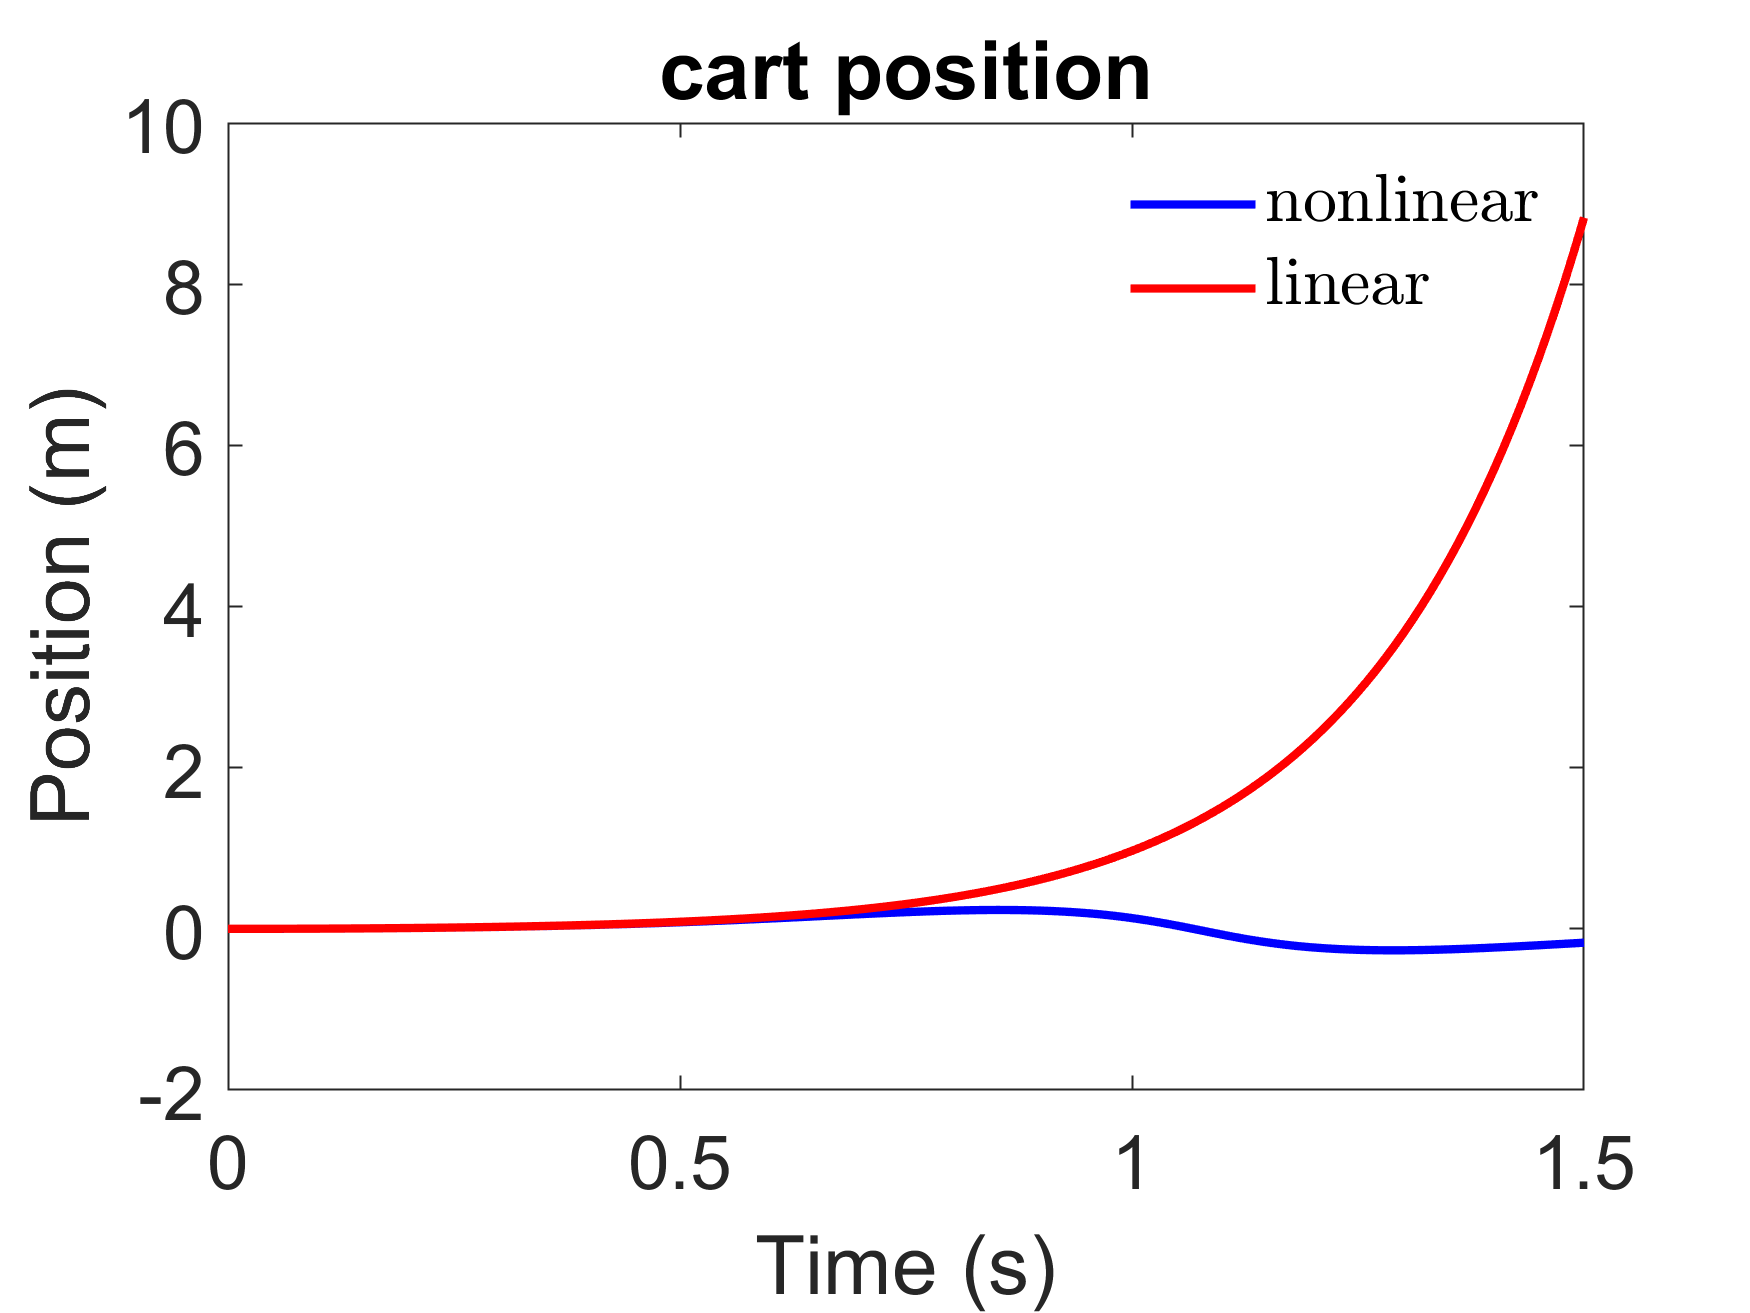
\includegraphics[width=0.6\textwidth]{w_open_loop.png}
    \caption{Non-linear and linear state space model simulations of $w(t)$ for zero input.}
    \label{fig:1}
\end{figure}

\begin{figure}[!ht]
    \centering
    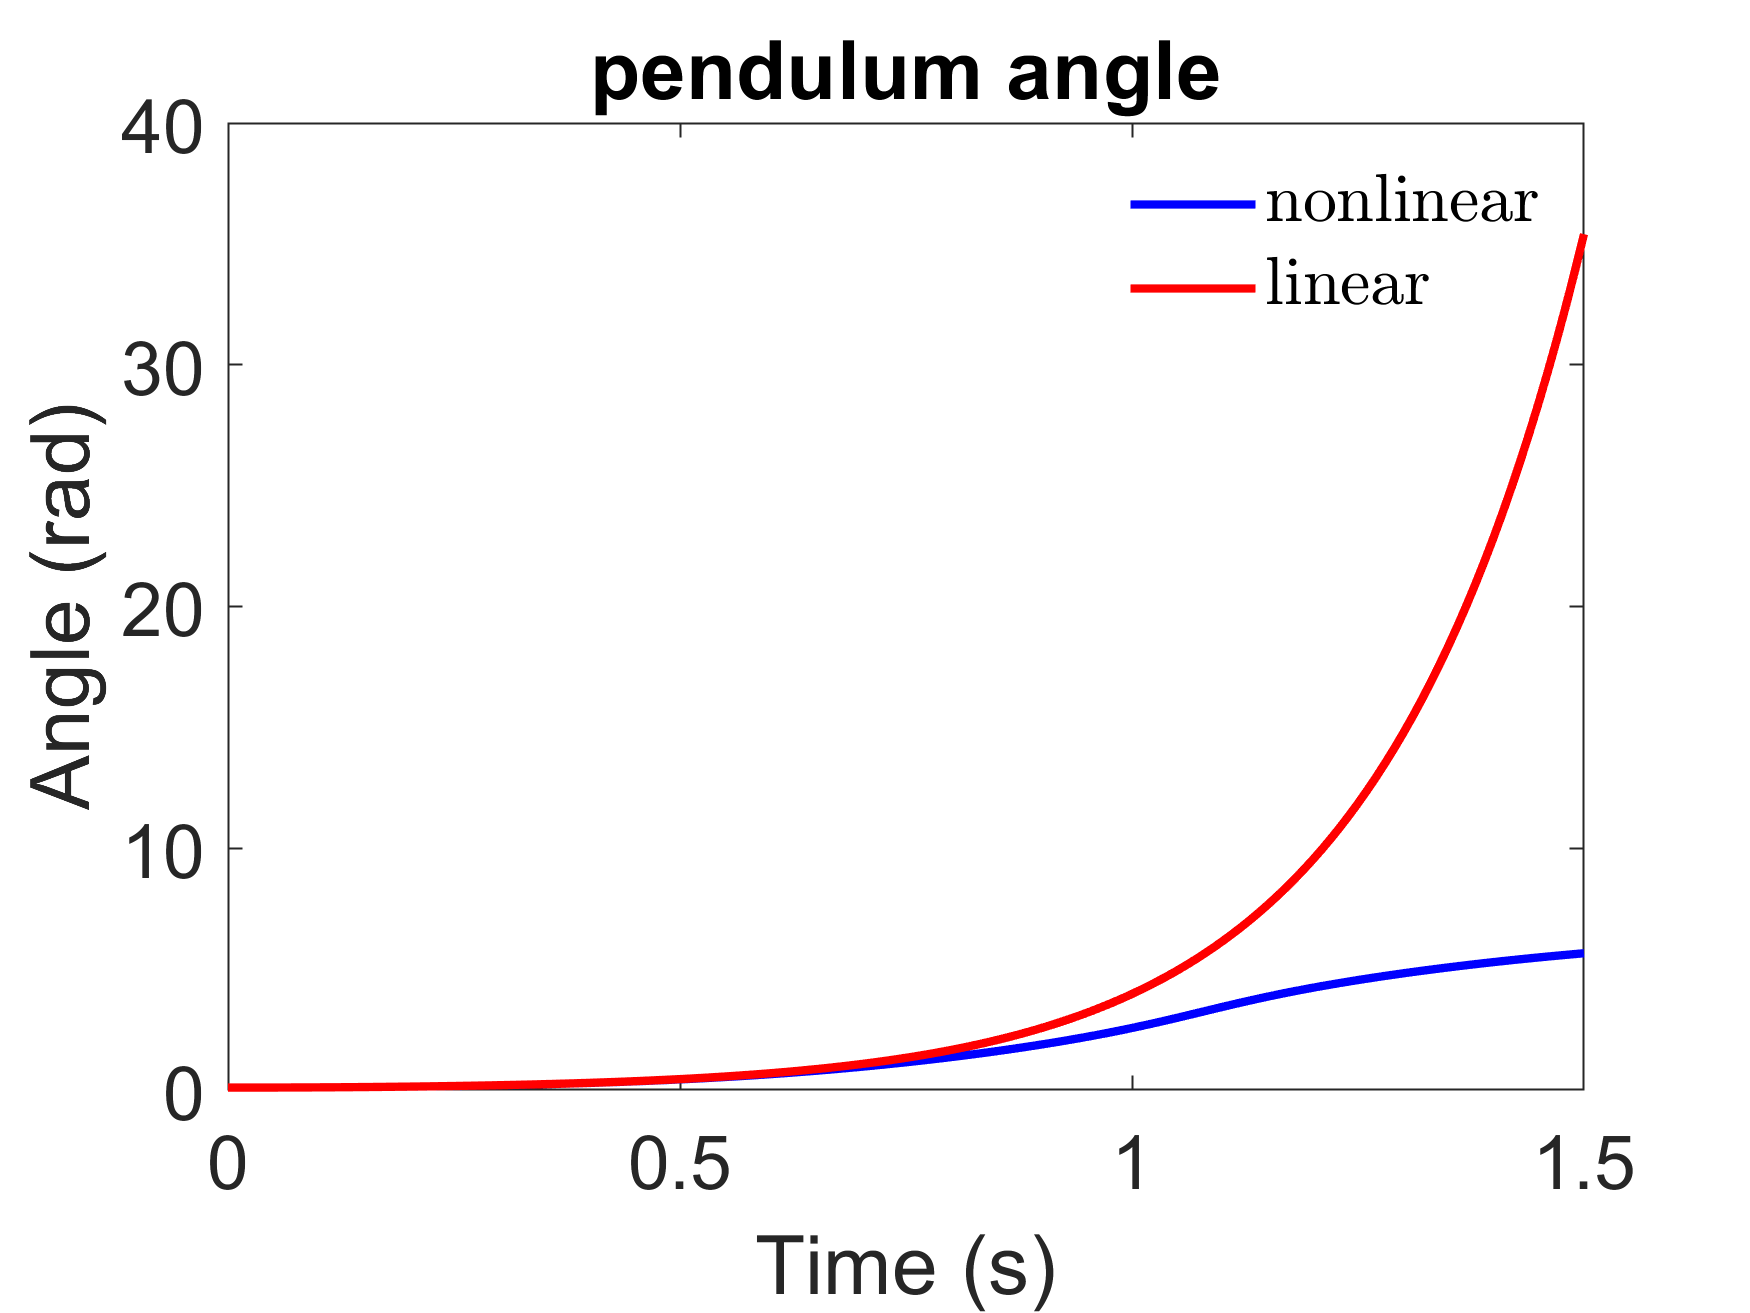
\includegraphics[width=0.6\textwidth]{theta_open_loop.png}
    \caption{Non-linear and linear state space model simulations of $\theta(t)$ for zero input.}
    \label{fig:2}
\end{figure}

\begin{figure}[!ht]
    \centering
    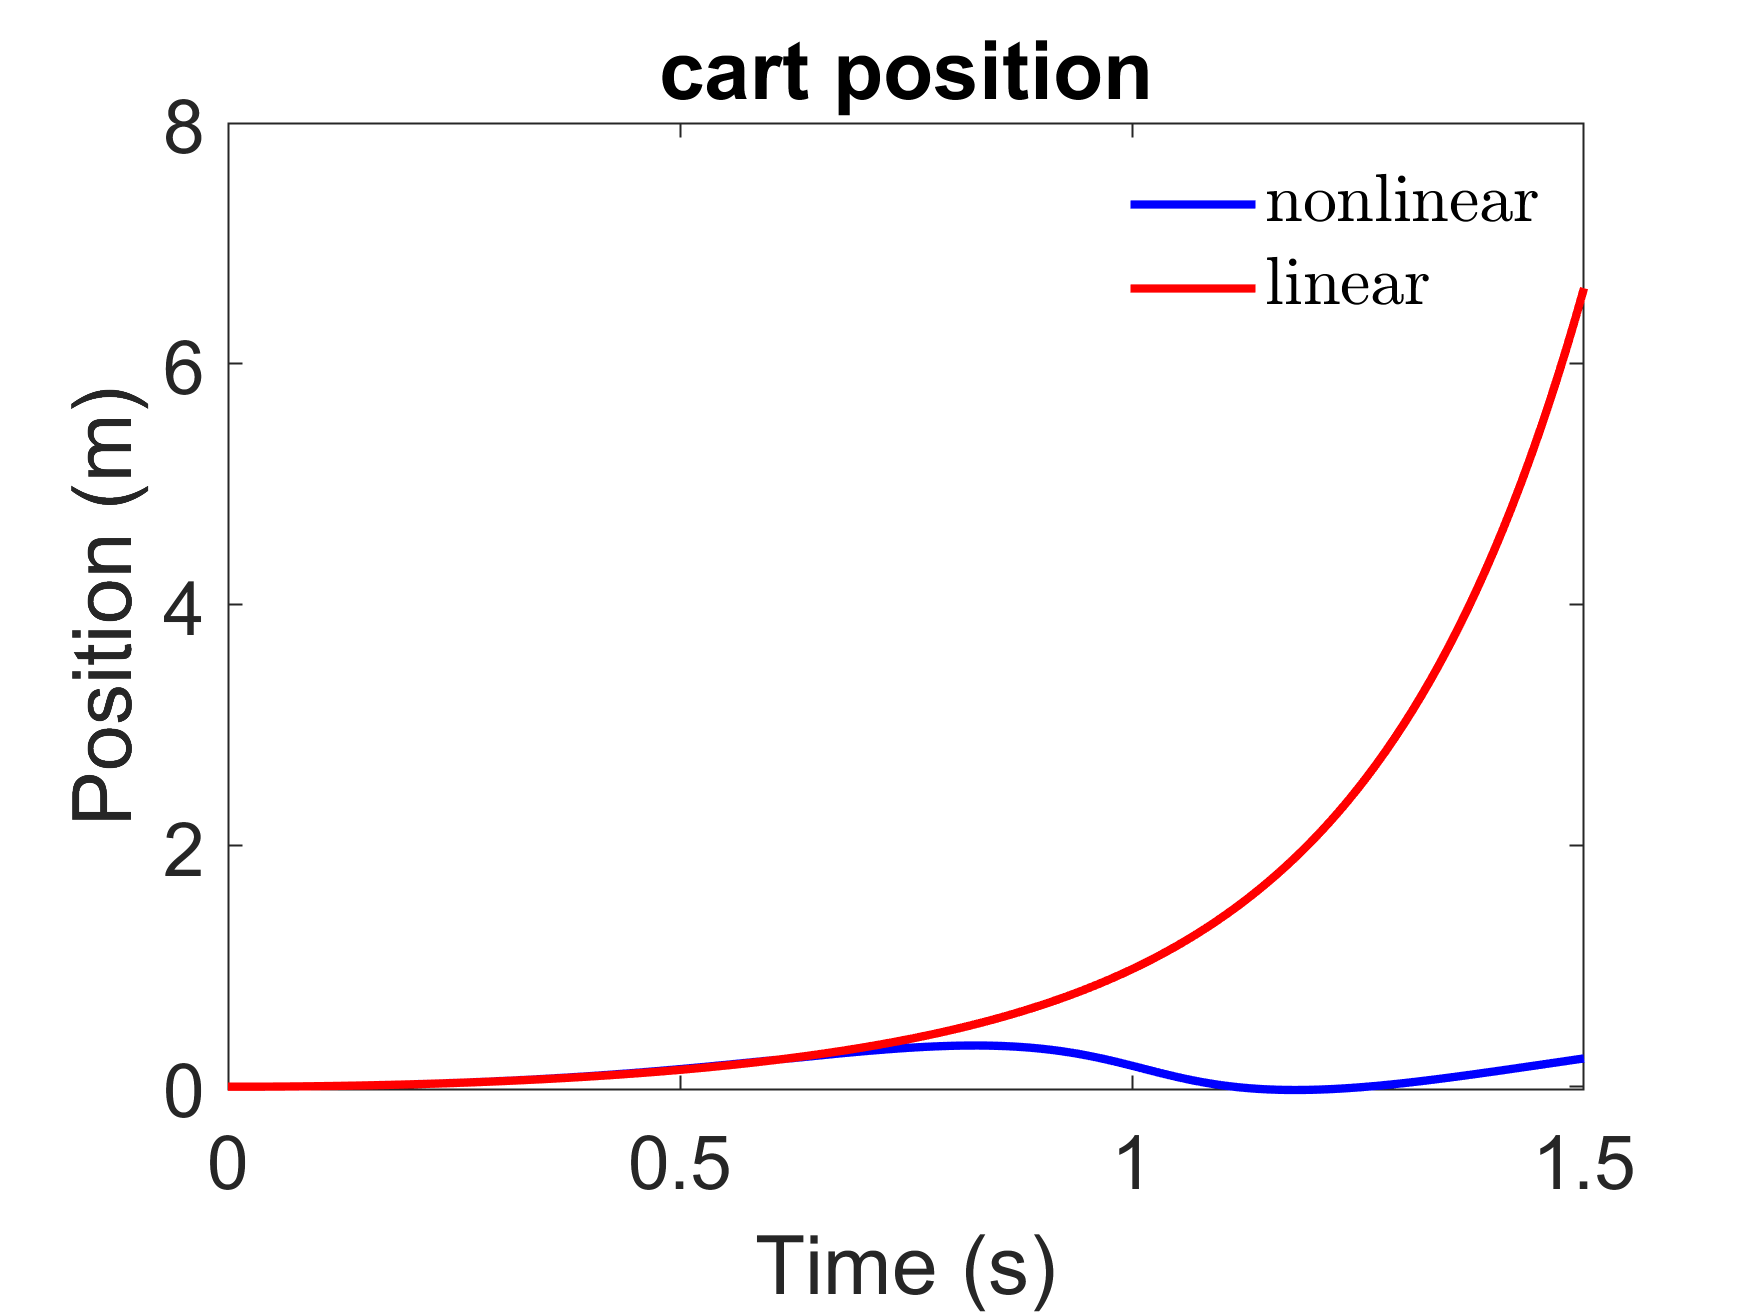
\includegraphics[width=0.6\textwidth]{w_open_loop_step_input.png}
    \caption{Non-linear and linear state space model simulations of $w(t)$ for step function input.}
    \label{fig:3}
\end{figure}

\begin{figure}[!ht]
    \centering
    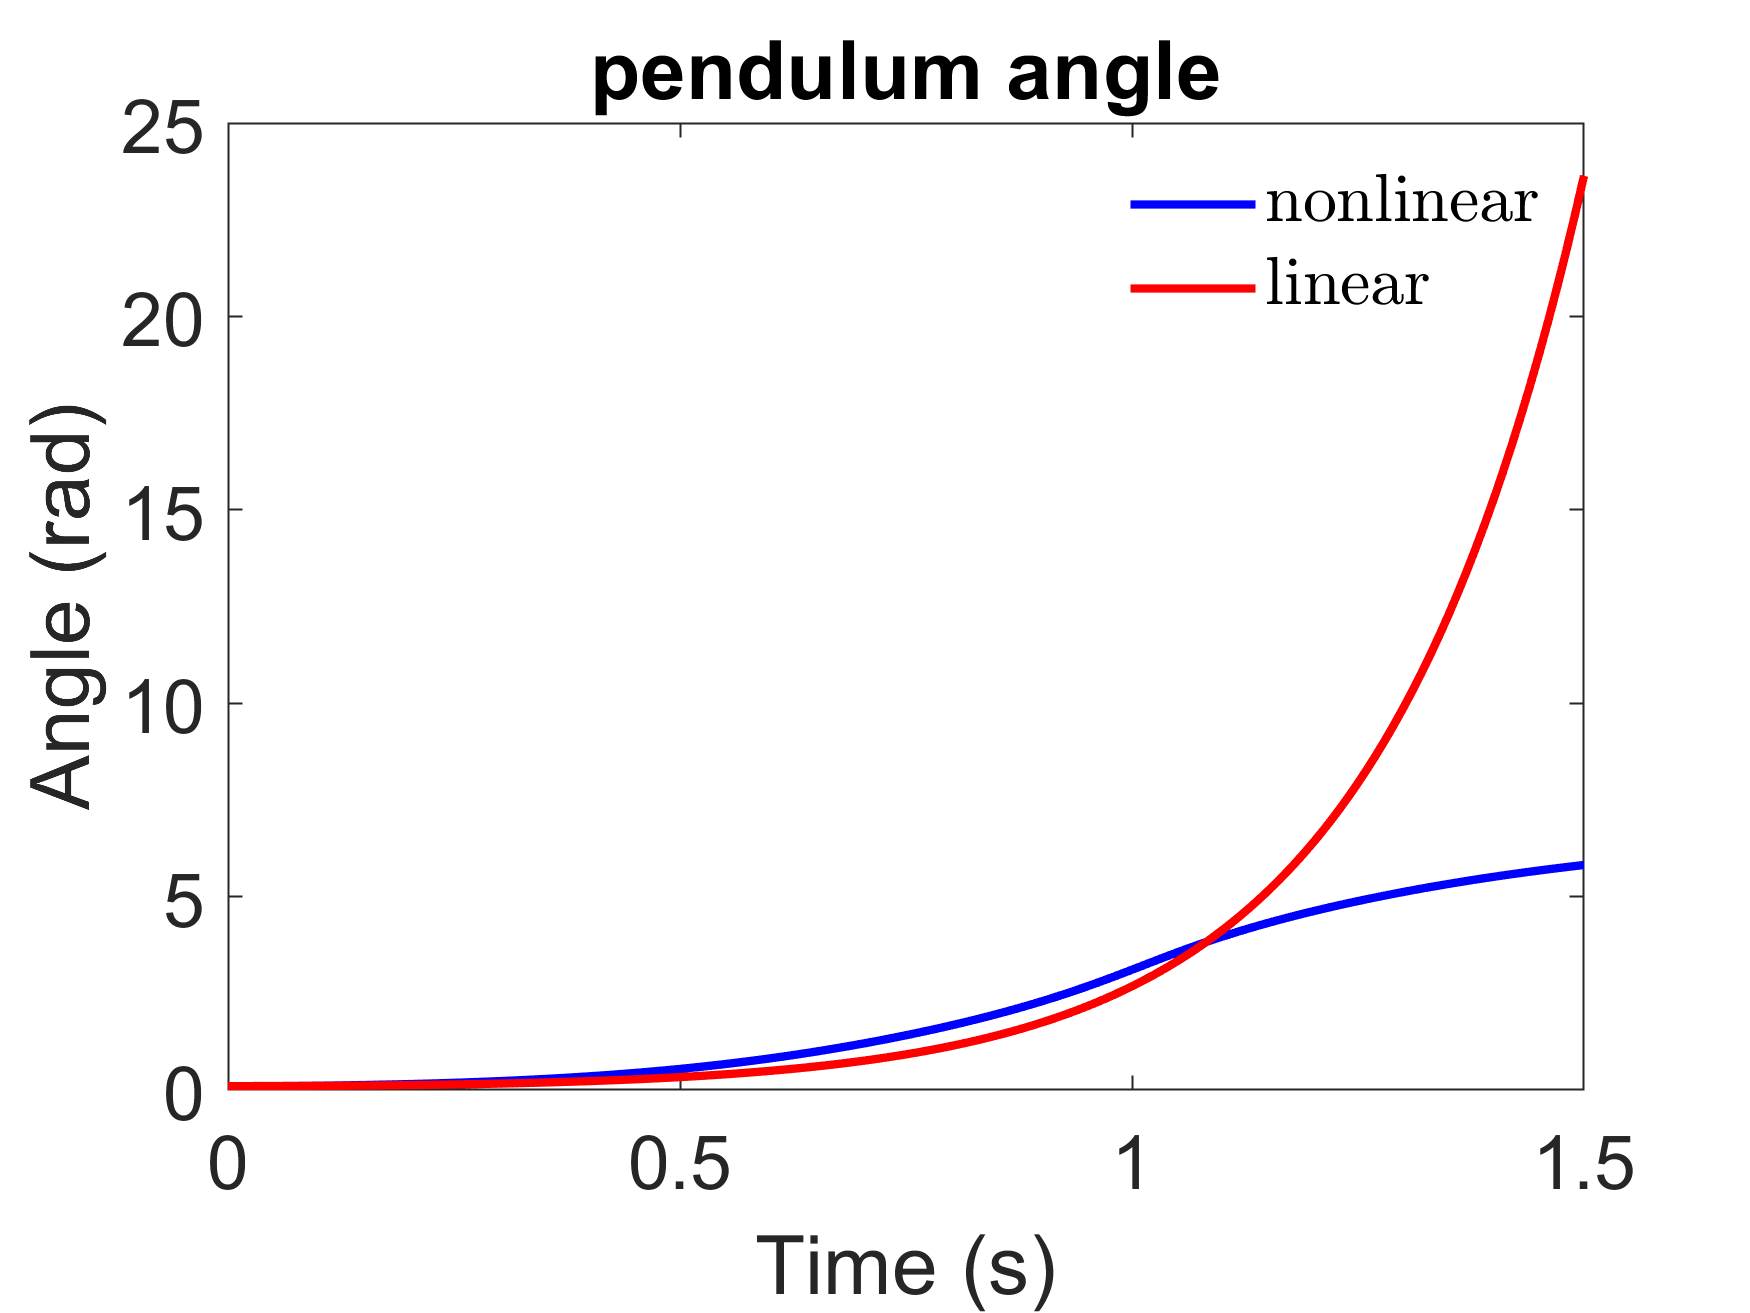
\includegraphics[width=0.6\textwidth]{theta_open_loop_step_input.png}
    \caption{Non-linear and linear state space model simulations of $\theta(t)$ for step function input.}
    \label{fig:4}
\end{figure}

\begin{figure}[!ht]
    \centering
    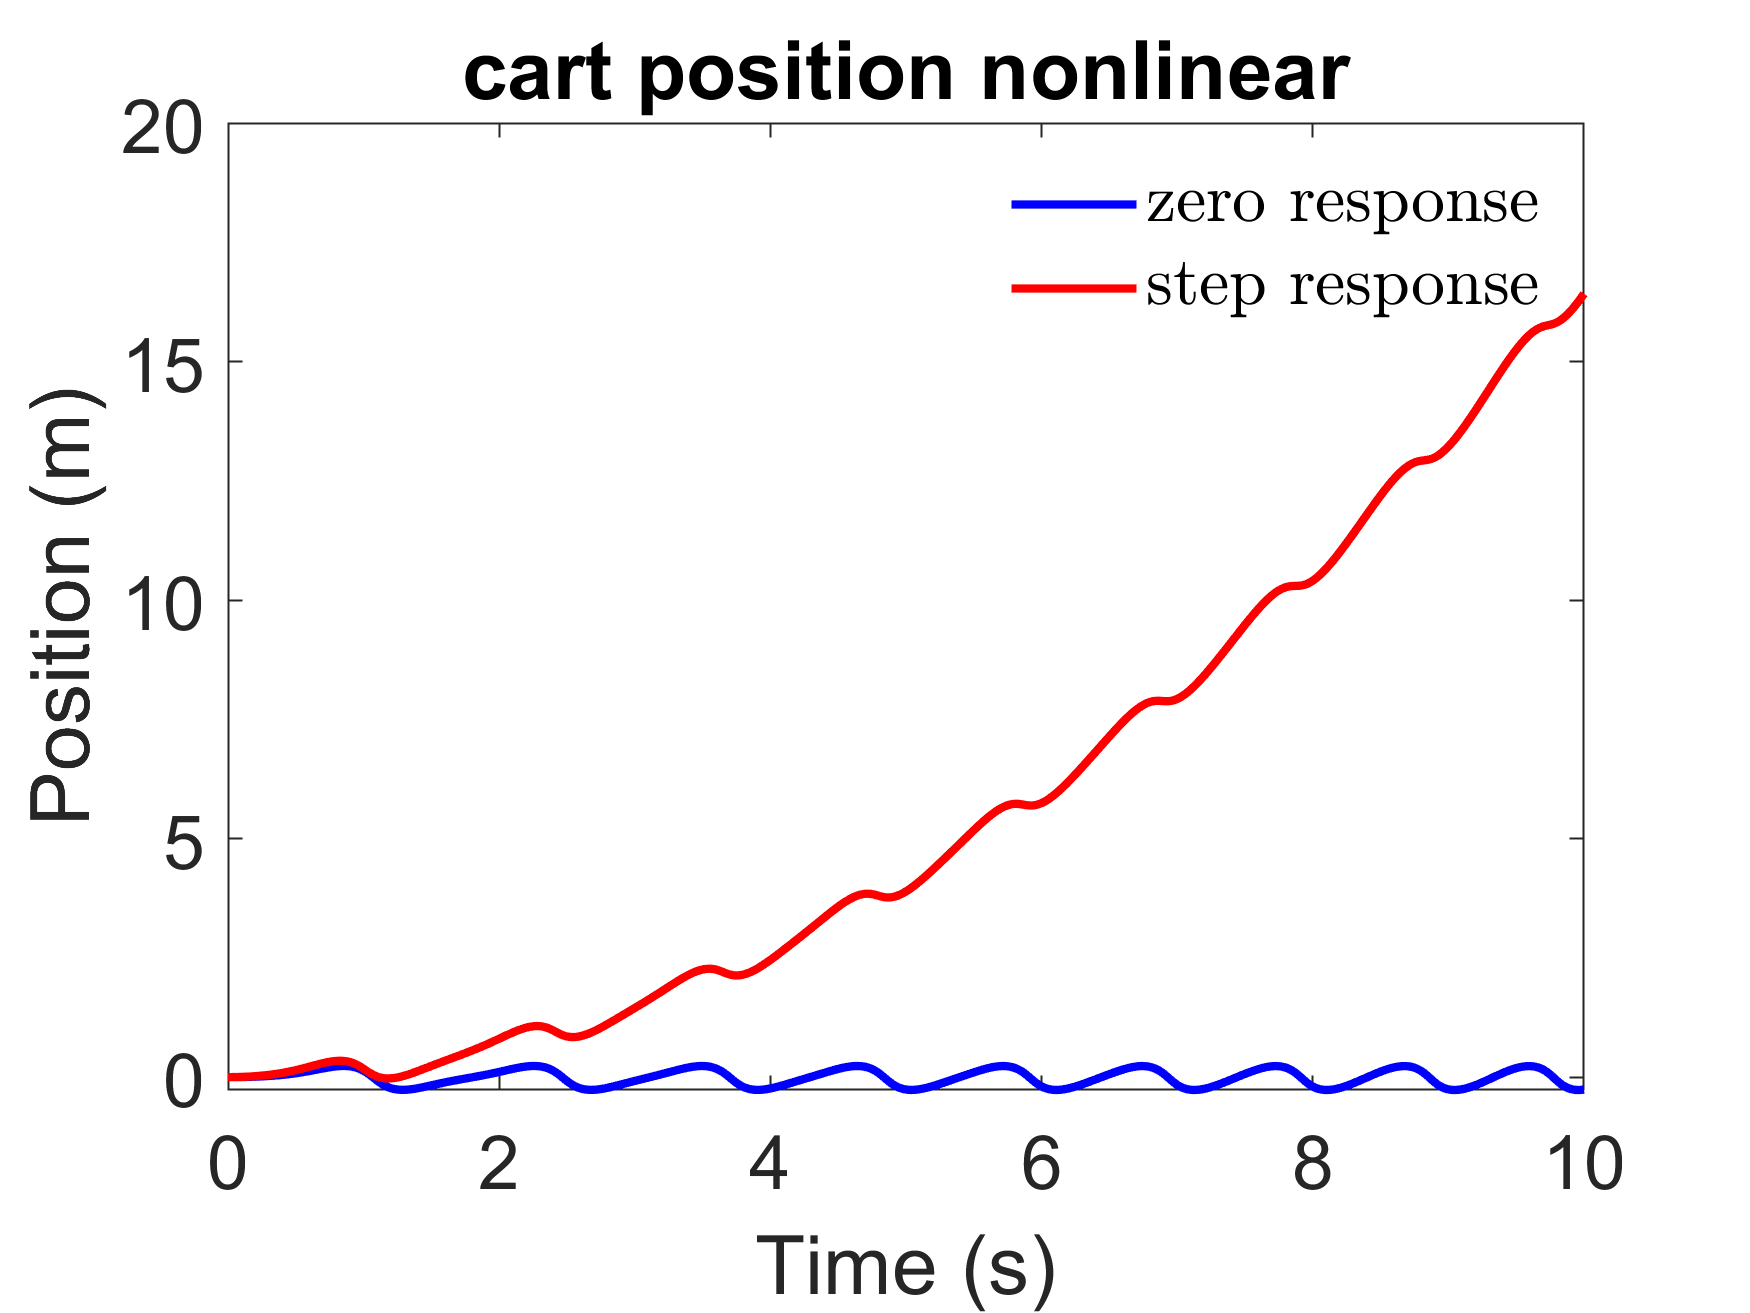
\includegraphics[width=0.6\textwidth]{nonlinear_zero_vs_step_w.png}
    \caption{Non-linear simulation results for cart position for zero input and step input.}
    \label{fig:5}
\end{figure}

\begin{figure}[!ht]
    \centering
    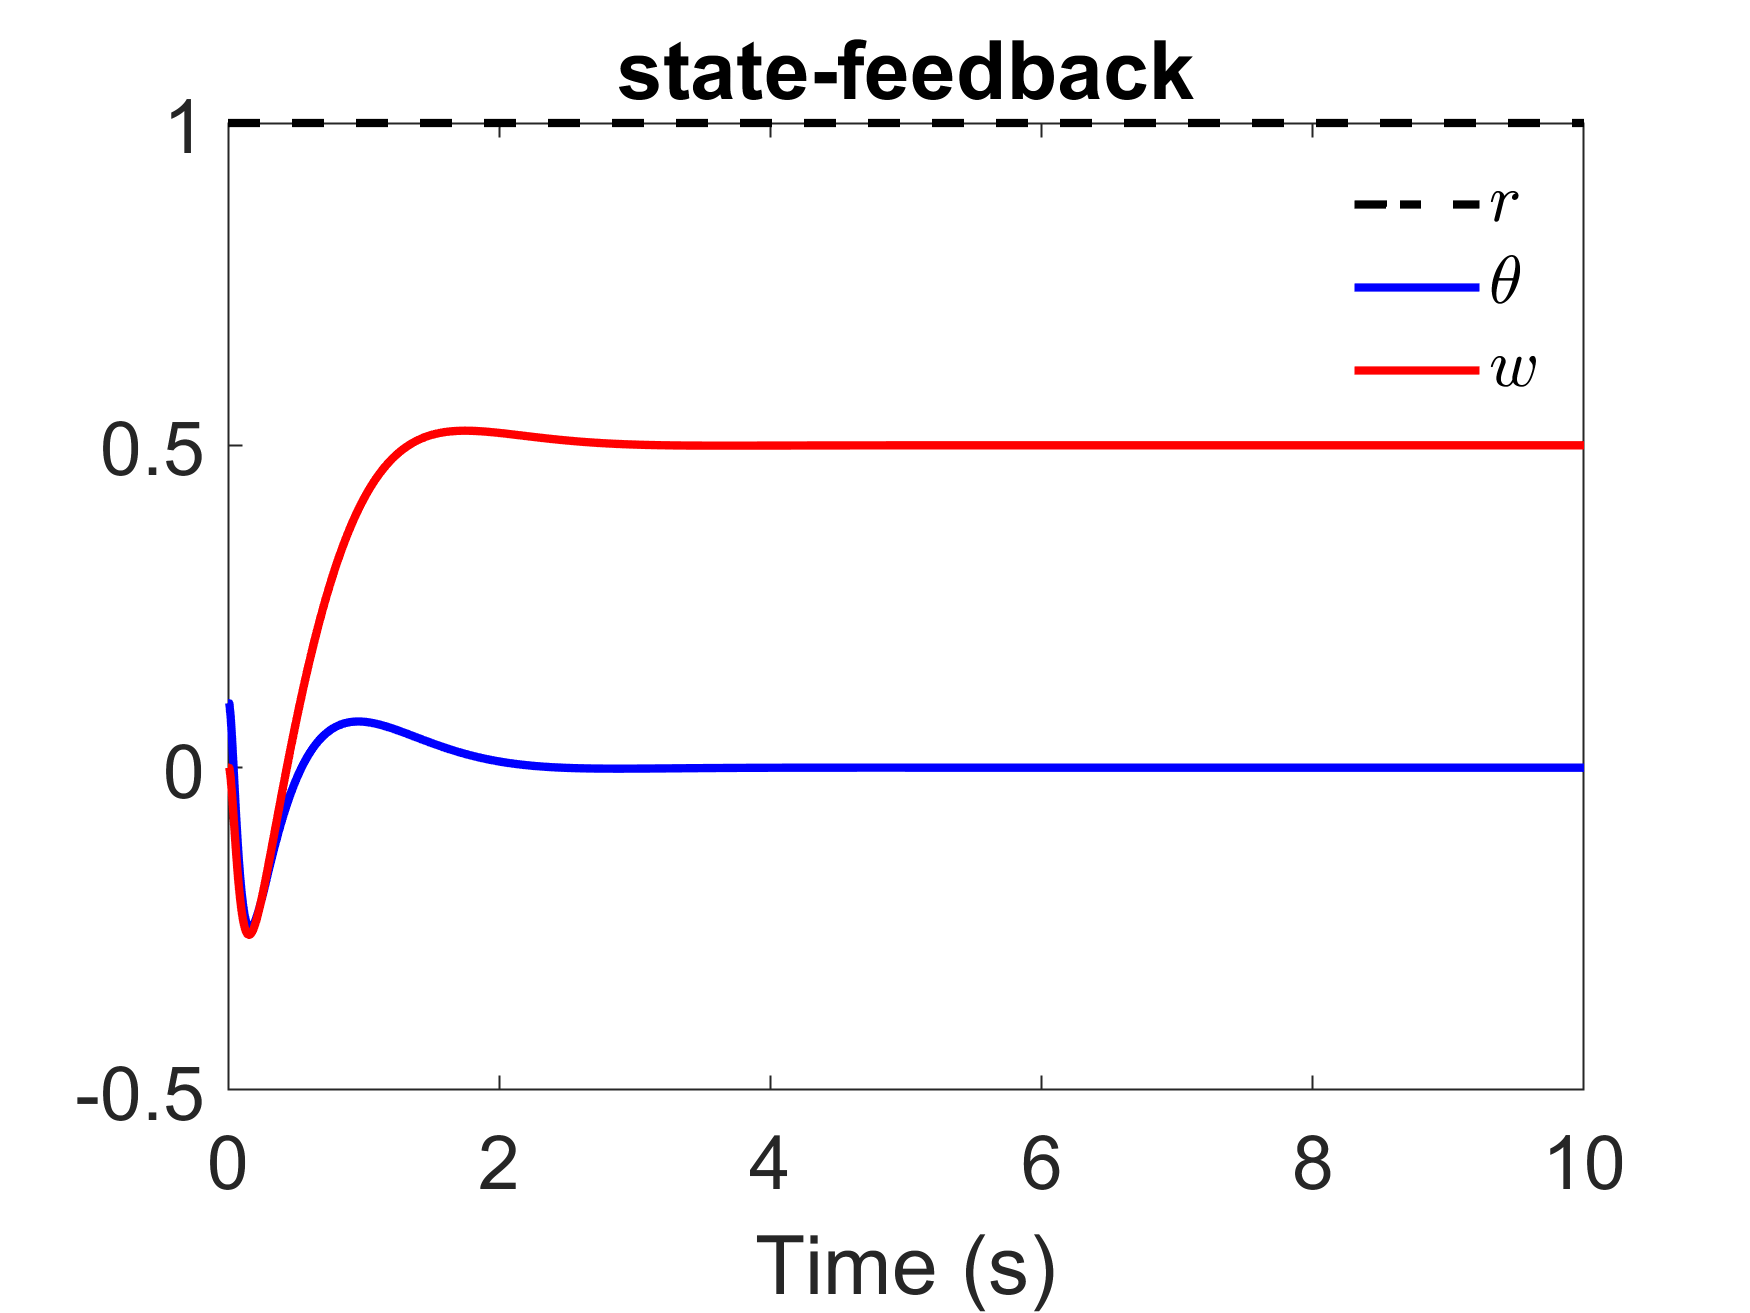
\includegraphics[width=0.6\textwidth]{state_feedback_1.png}
    \caption{State feedback for $y(0) = [0.1, 0]^T$, $y(\infty) = [0, 0.5]^T$.}
    \label{fig:6}
\end{figure}

\begin{figure}[!ht]
    \centering
    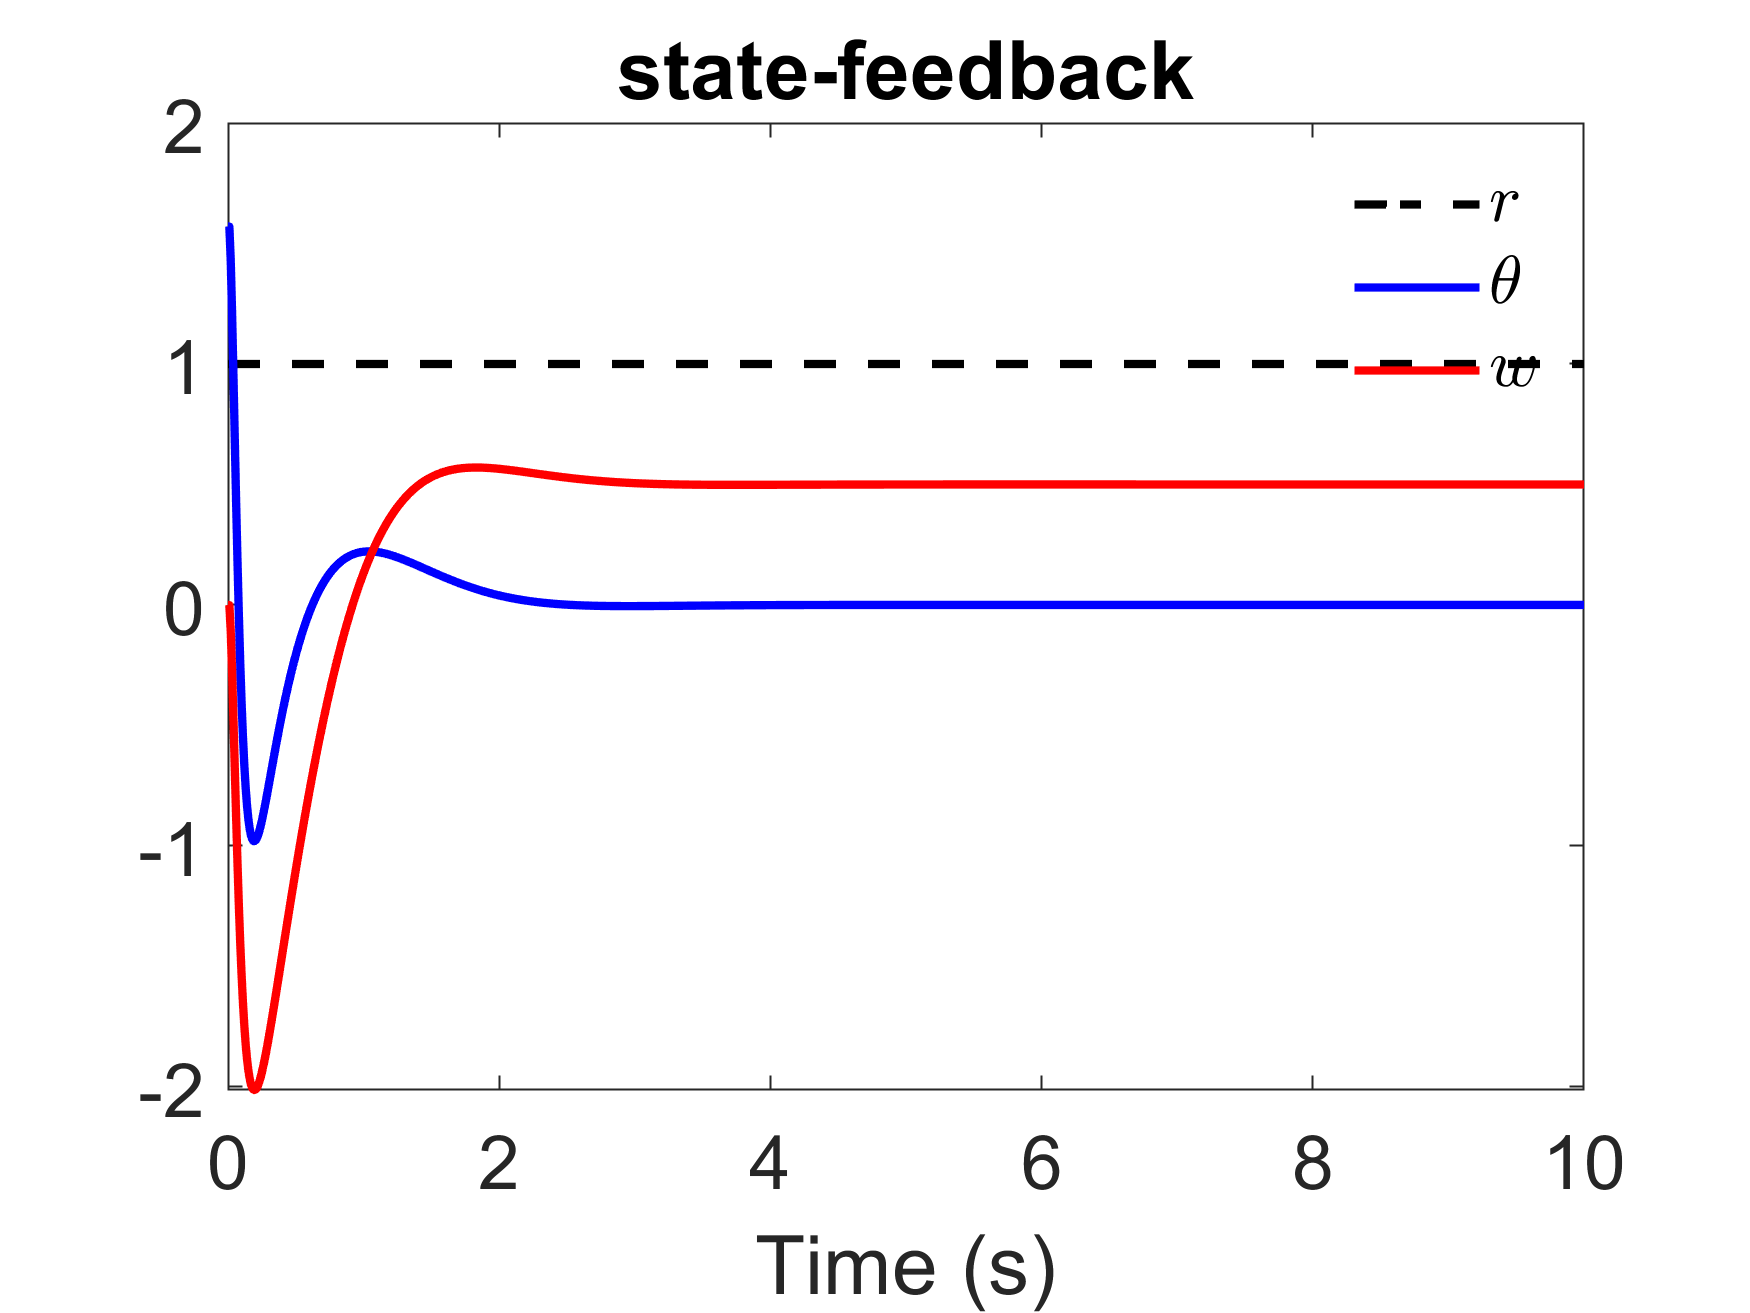
\includegraphics[width=0.6\textwidth]{state_feedback_2.png}
    \caption{State feedback for $y(0) = [\pi/2, 0]^T$, $y(\infty) = [0, 0.5]^T$.}
    \label{fig:7}
\end{figure}

\begin{figure}[!ht]
    \centering
    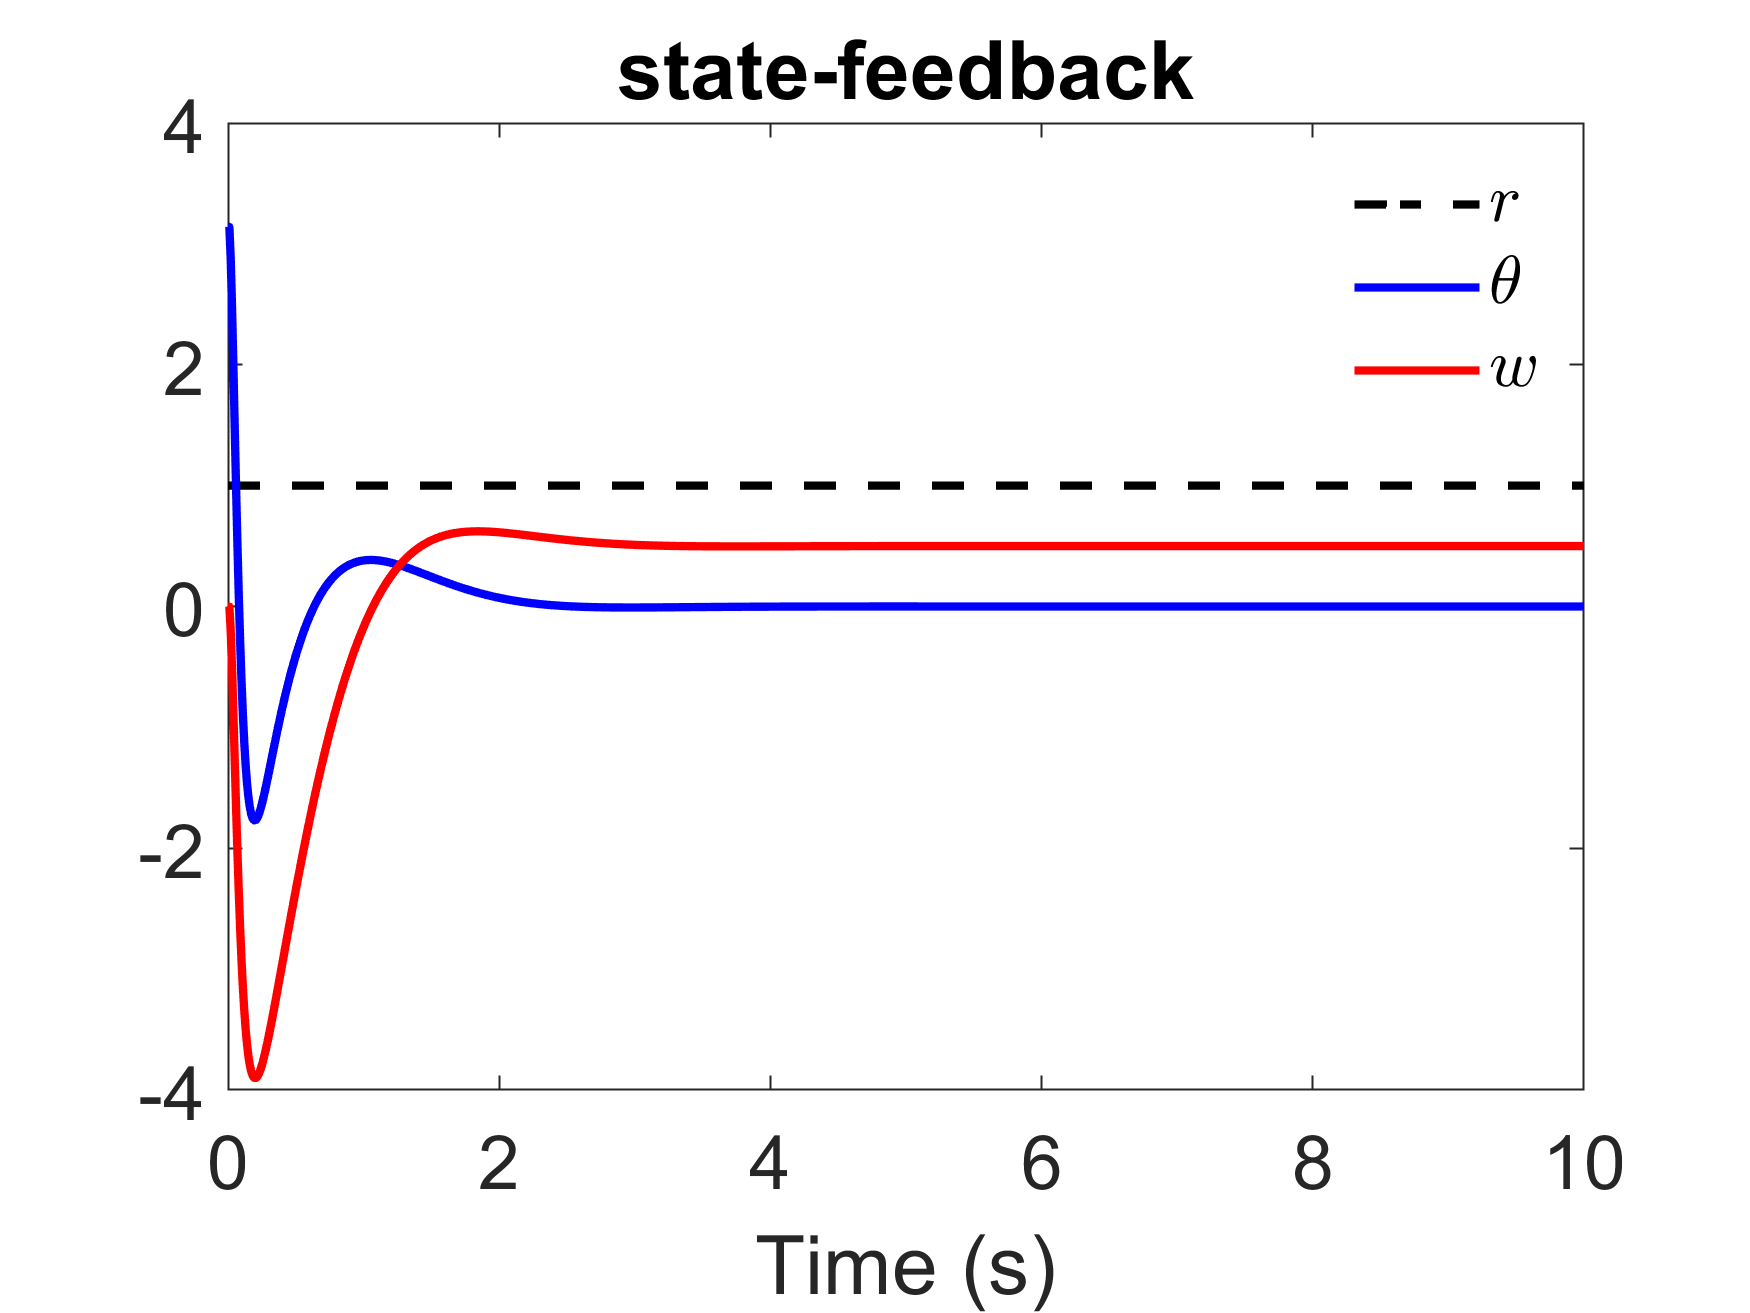
\includegraphics[width=0.6\textwidth]{state_feedback_3.png}
    \caption{State feedback for $y(0) = [\pi, 0]^T$, $y(\infty) = [0, 0.5]^T$.}
    \label{fig:8}
\end{figure}

\begin{figure}[!ht]
    \centering
    \includegraphics[width=0.6\textwidth]{single_output_observer/fig1.png}
    \caption{Single $y = w$, observer control.}
    \label{fig:observer_sim_first}
\end{figure}

\begin{figure}[!ht]
    \centering
    \includegraphics[width=0.6\textwidth]{single_output_observer/fig2.png}
    \caption{Single $y = w$, observer control.}
\end{figure}

\begin{figure}[!ht]
    \centering
    \includegraphics[width=0.6\textwidth]{single_output_observer/fig3.png}
    \caption{Single $y = w$, observer control.}
\end{figure}

\begin{figure}[!ht]
    \centering
    \includegraphics[width=0.6\textwidth]{single_output_observer/fig4.png}
    \caption{Single $y = w$, observer control.}
\end{figure}

\begin{figure}[!ht]
    \centering
    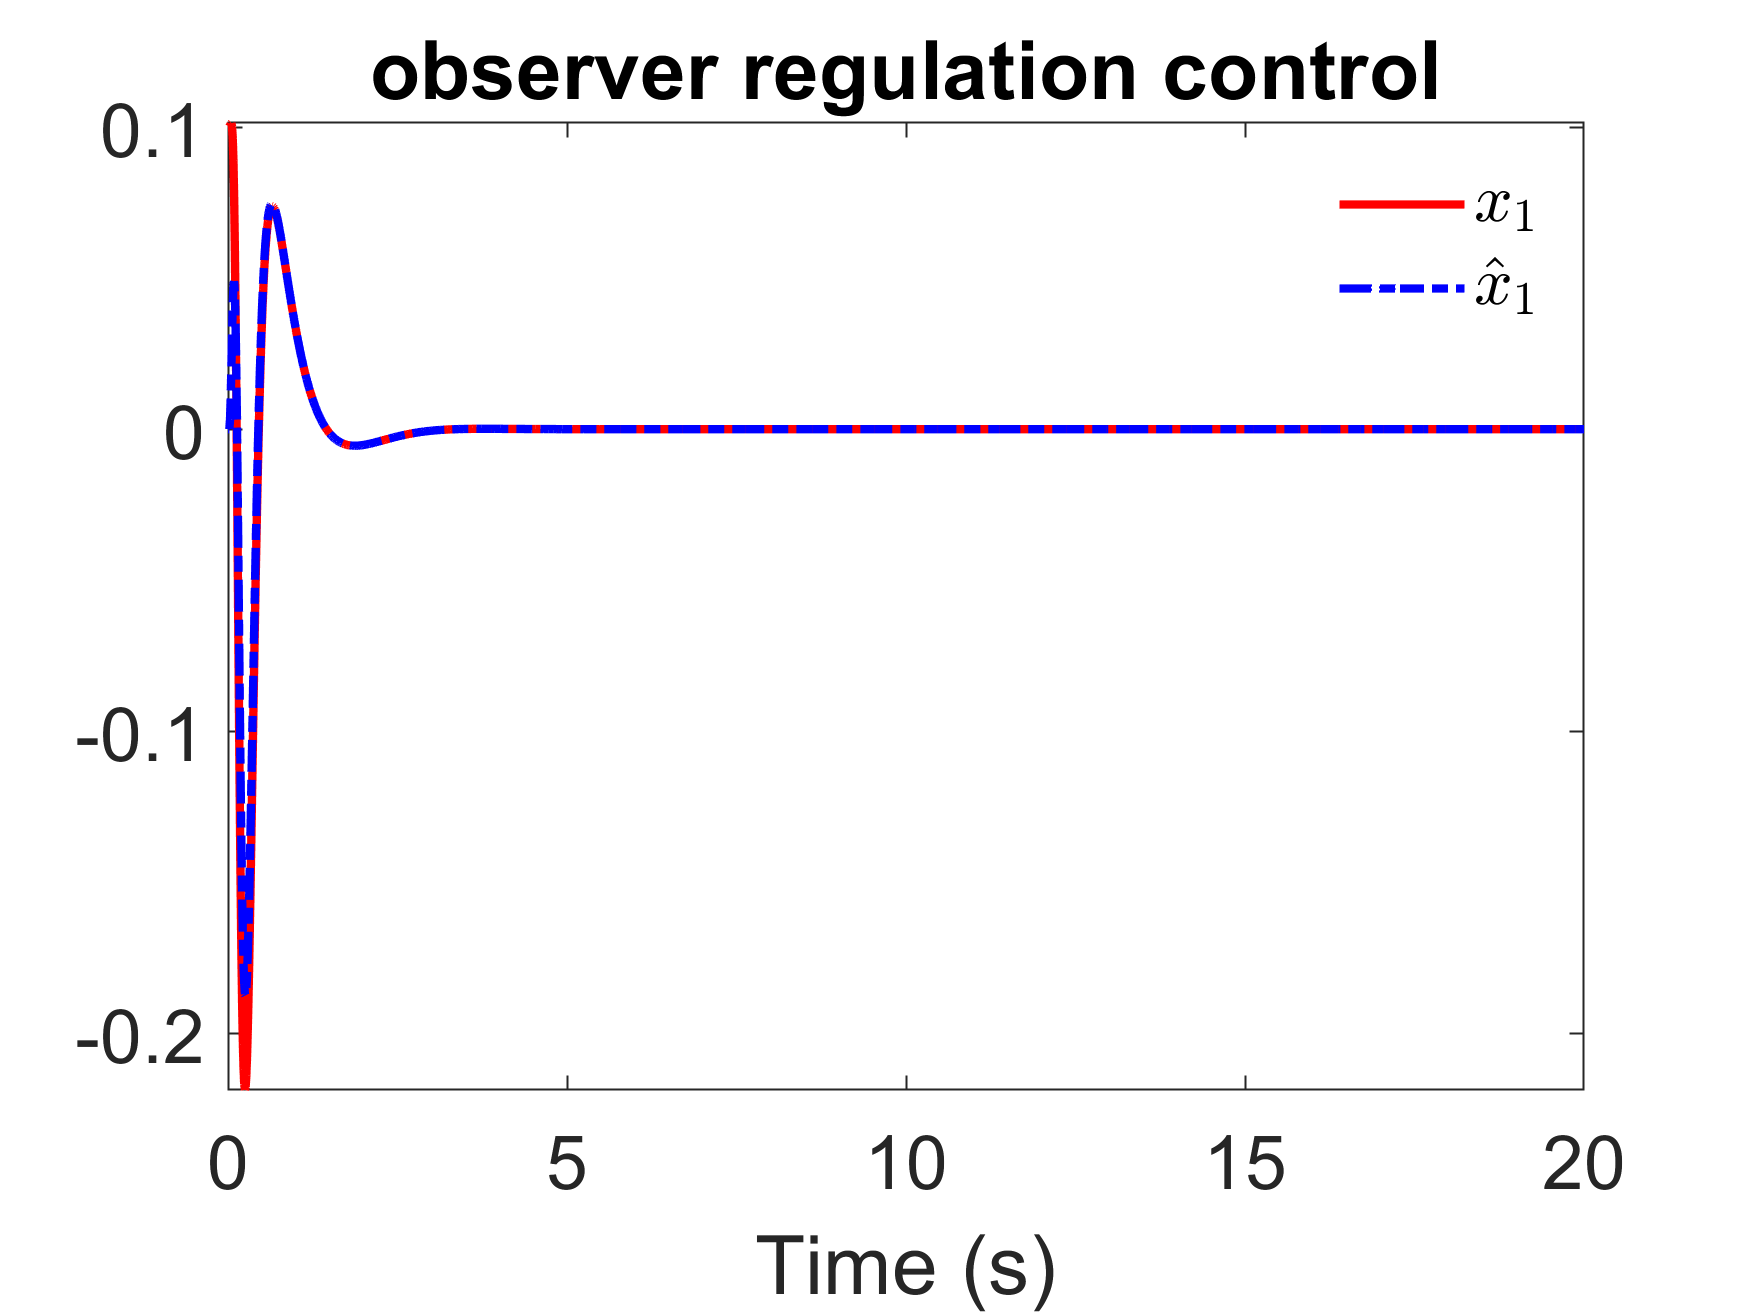
\includegraphics[width=0.6\textwidth]{single_output_observer/fig5.png}
    \caption{Single $y = w$, observer control.}
\end{figure}

\begin{figure}[!ht]
    \centering
    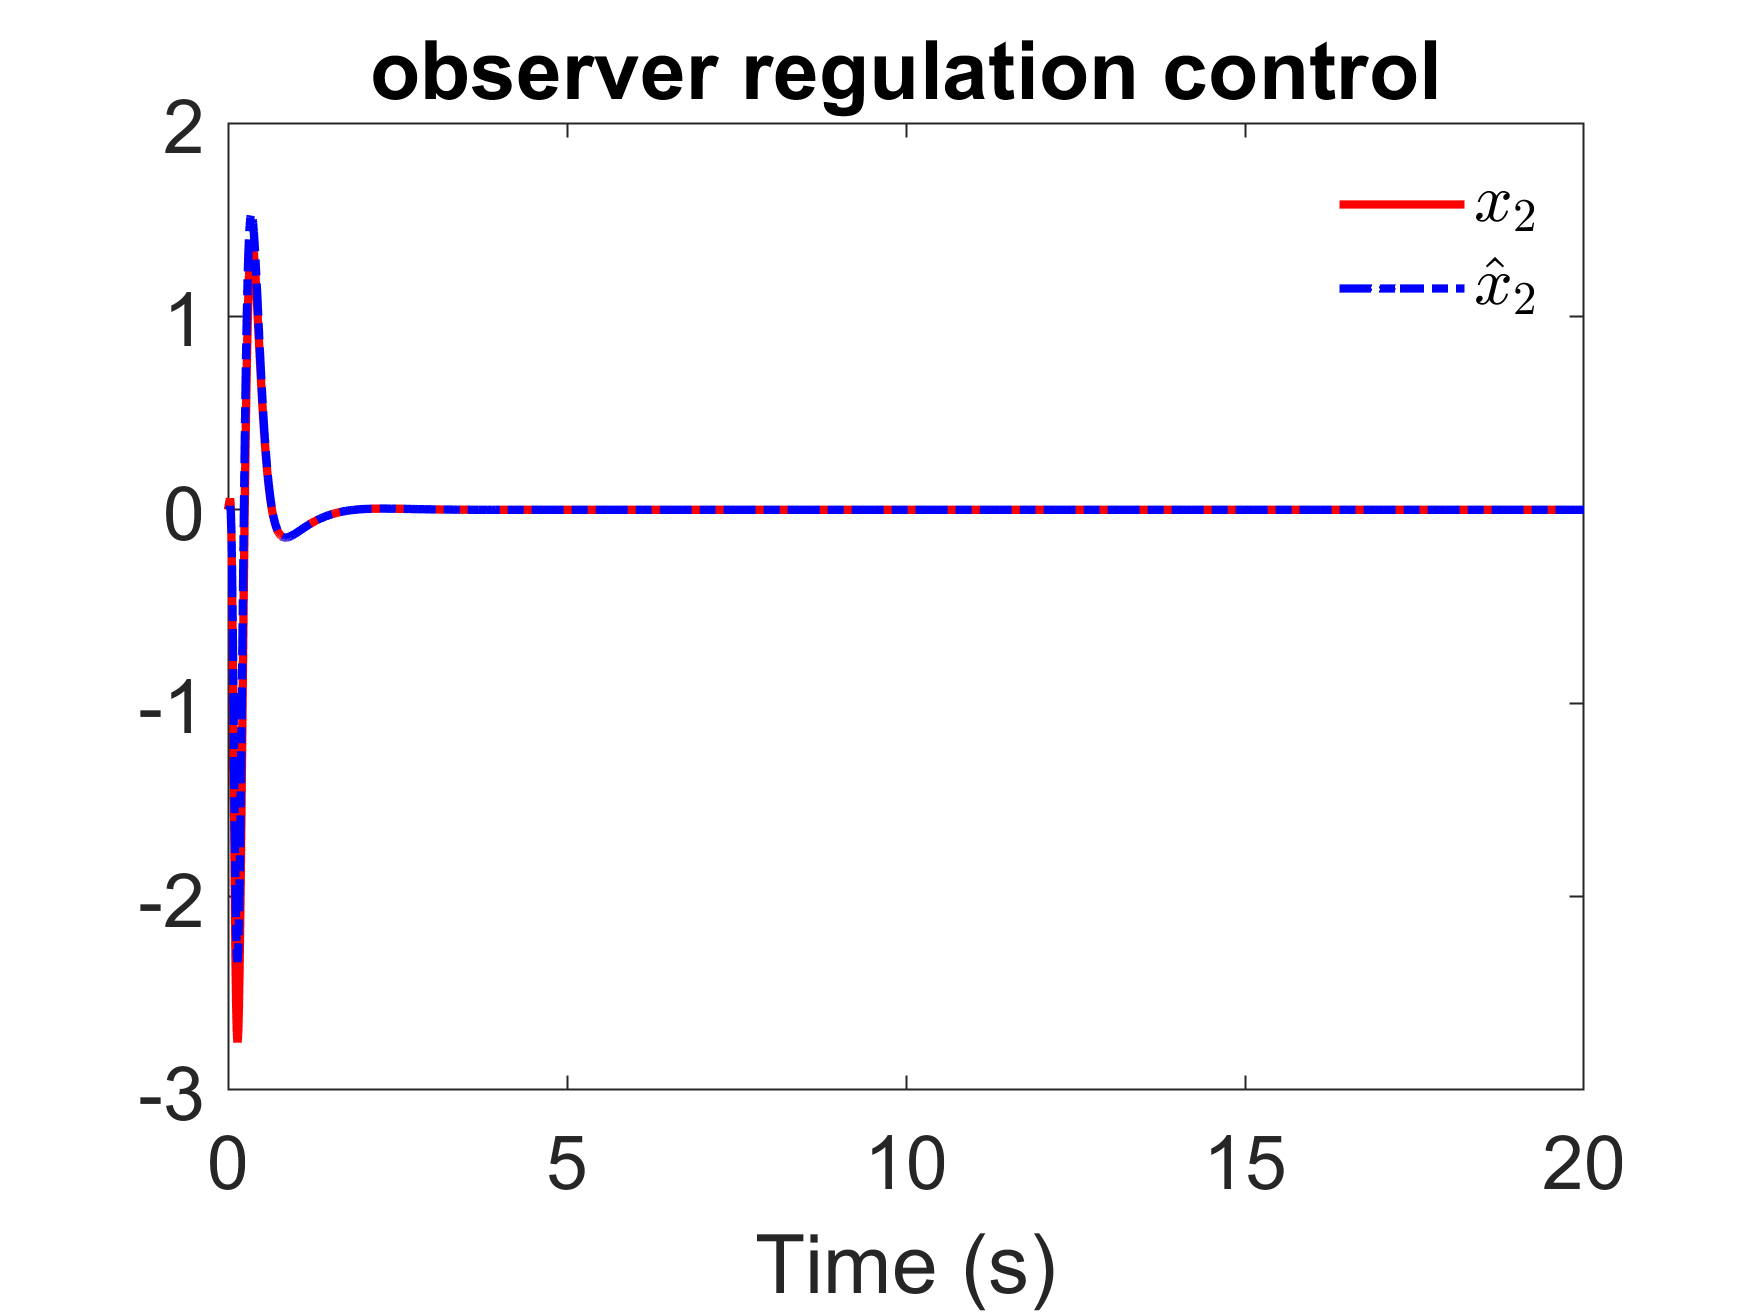
\includegraphics[width=0.6\textwidth]{single_output_observer/fig6.png}
    \caption{Single $y = w$, observer control.}
\end{figure}

\begin{figure}[!ht]
    \centering
    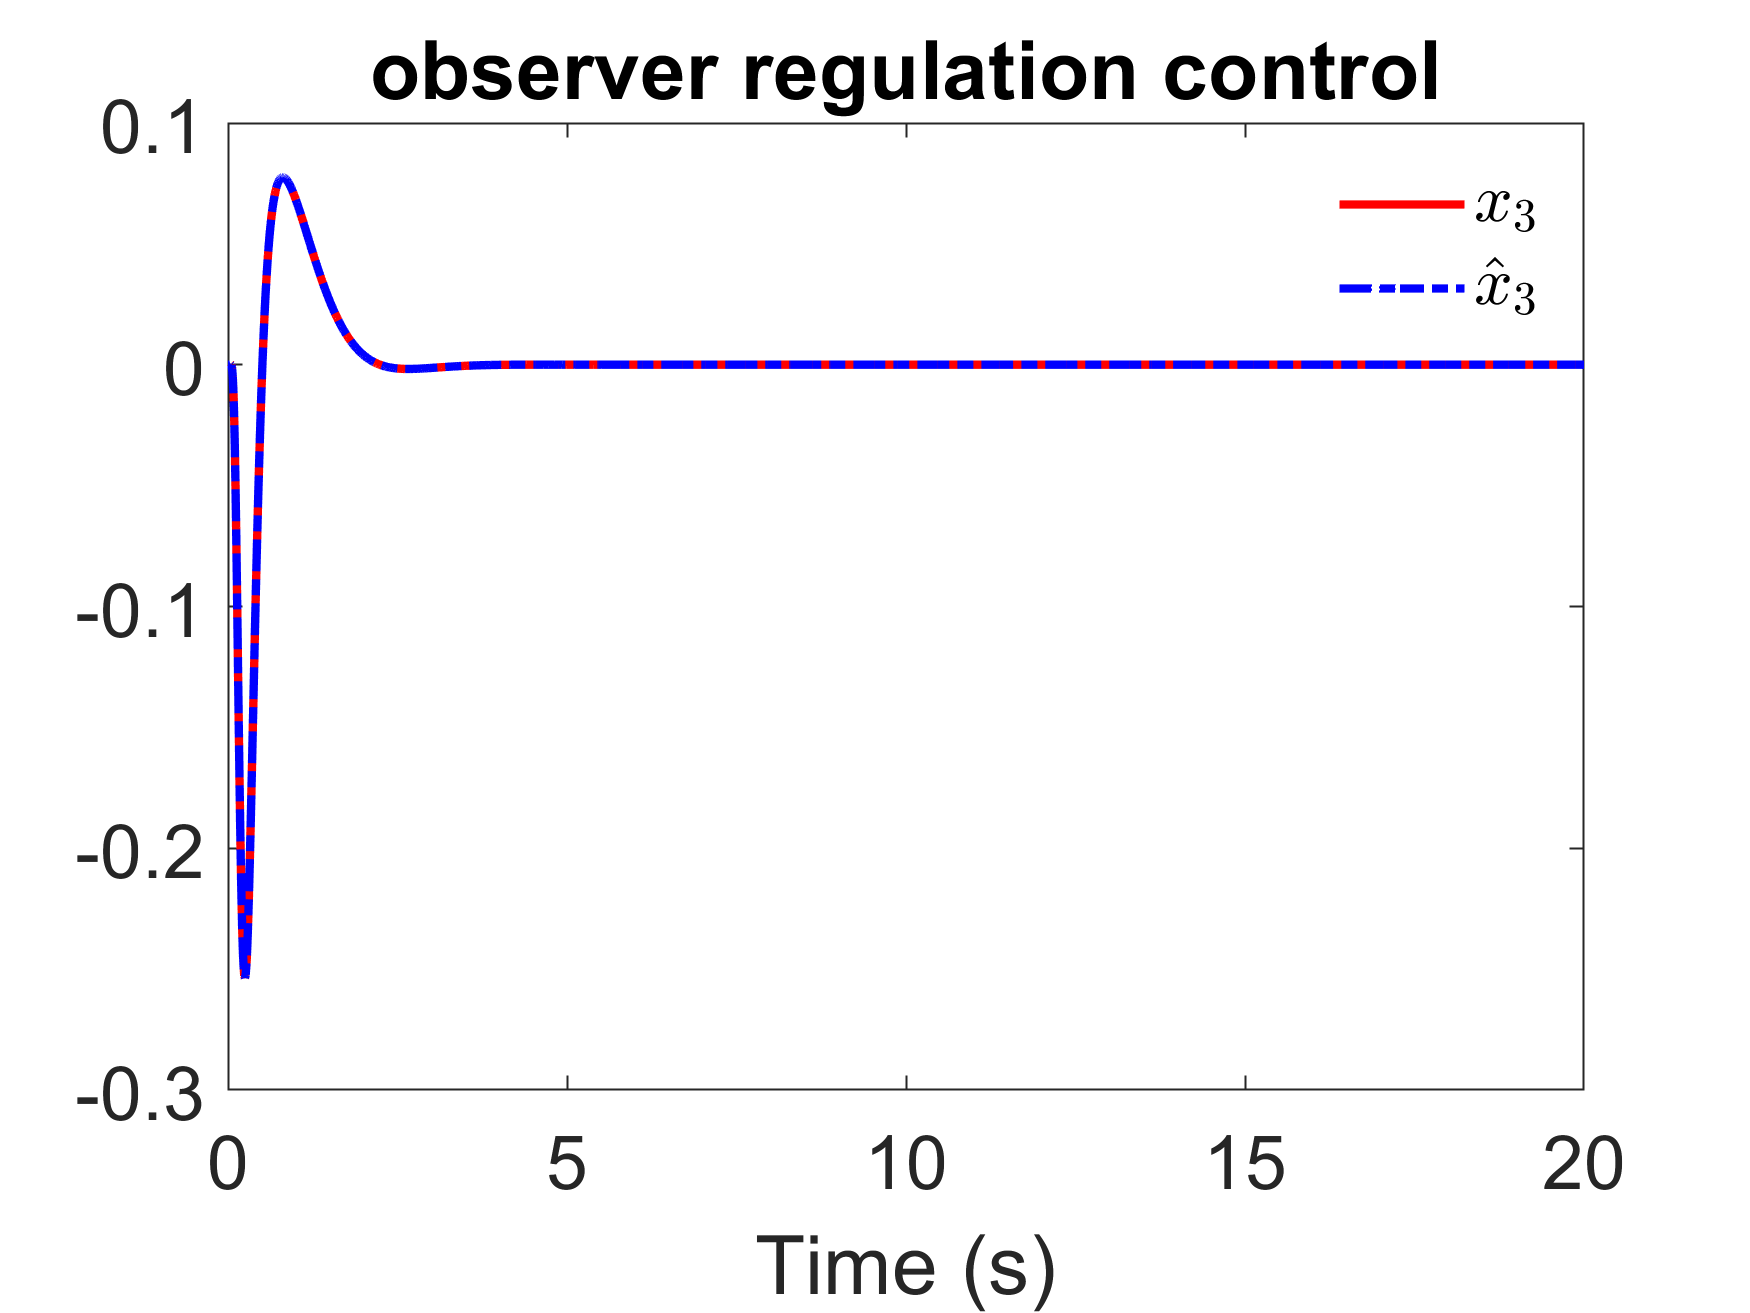
\includegraphics[width=0.6\textwidth]{single_output_observer/fig7.png}
    \caption{Single $y = w$, observer control.}
\end{figure}

\begin{figure}[!ht]
    \centering
    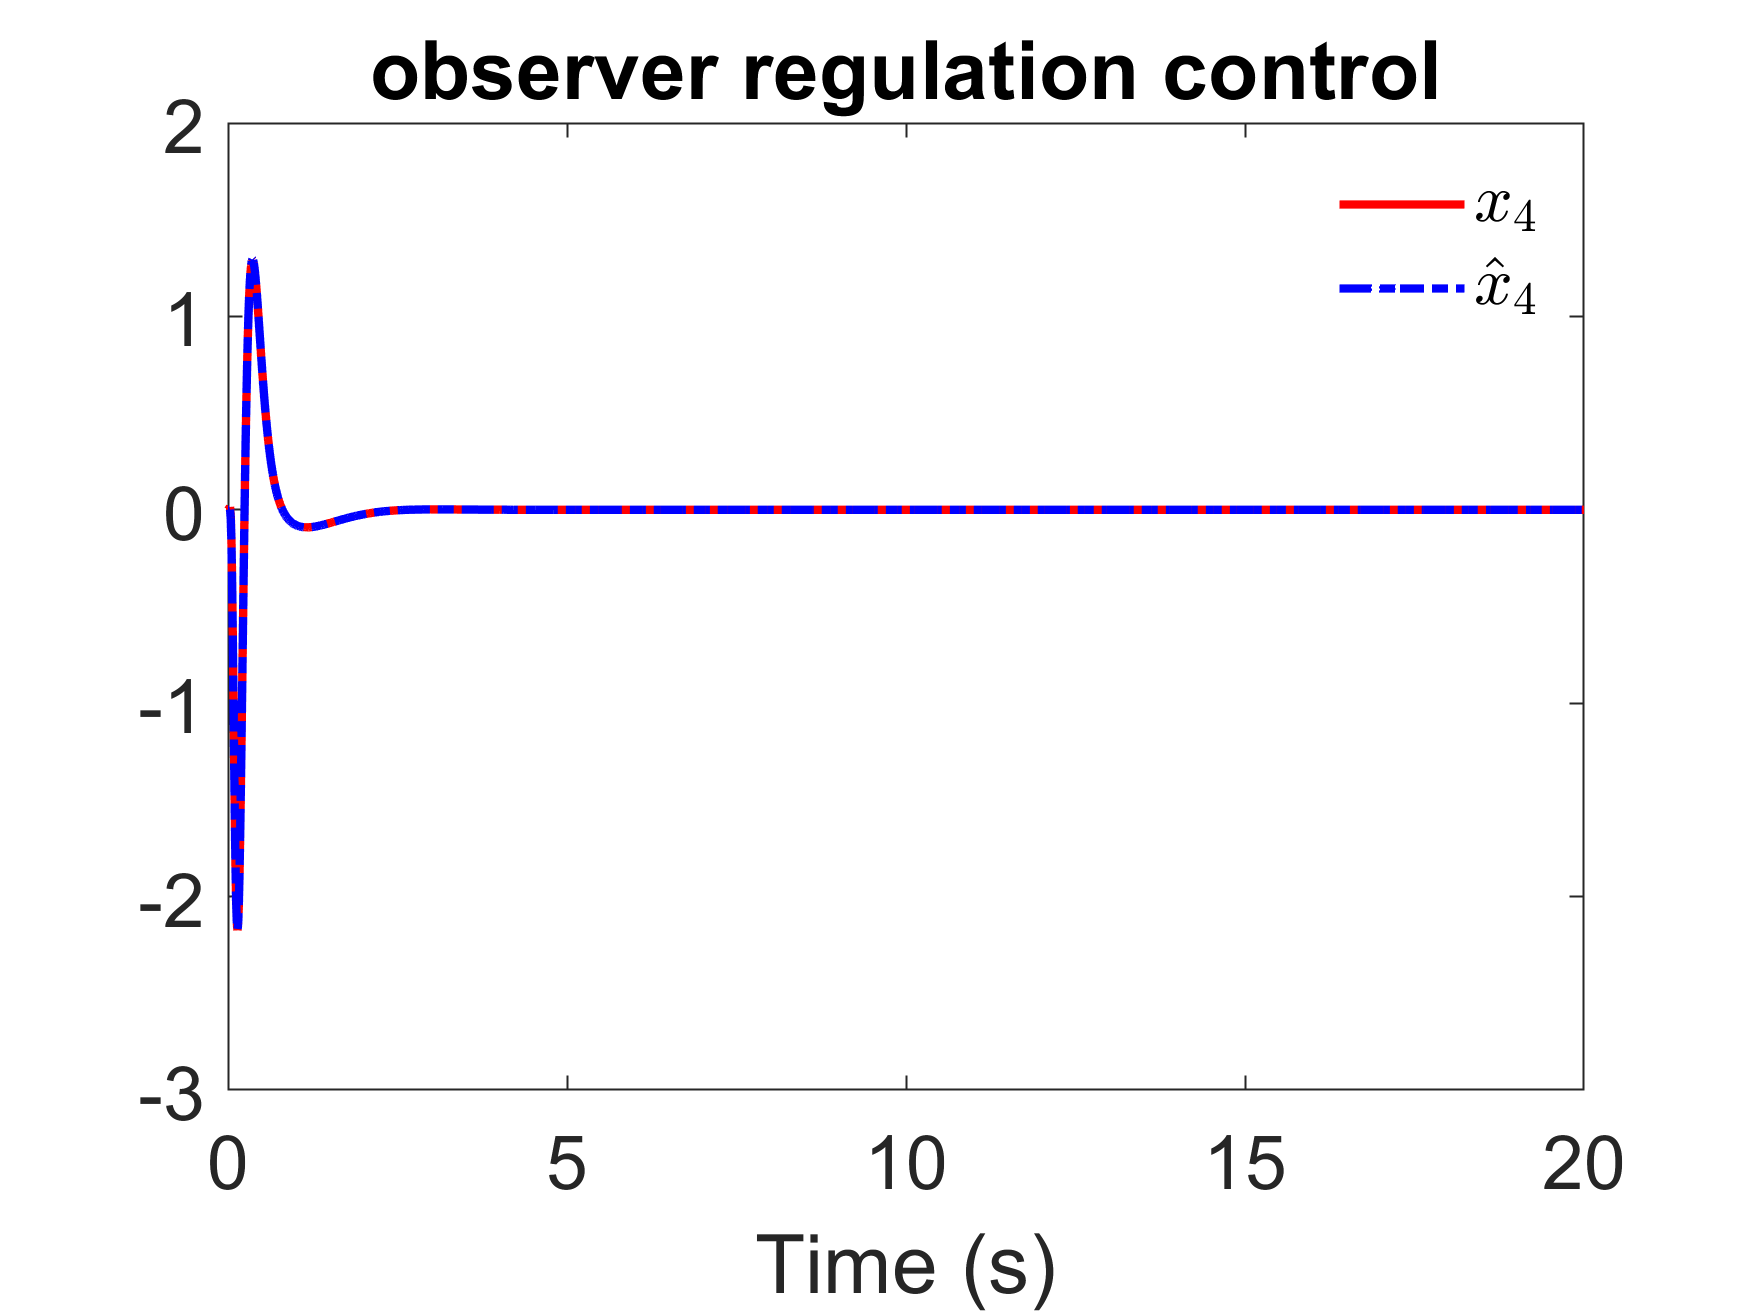
\includegraphics[width=0.6\textwidth]{single_output_observer/fig8.png}
    \caption{Single $y = w$, observer control.}
\end{figure}

\begin{figure}[!ht]
    \centering
    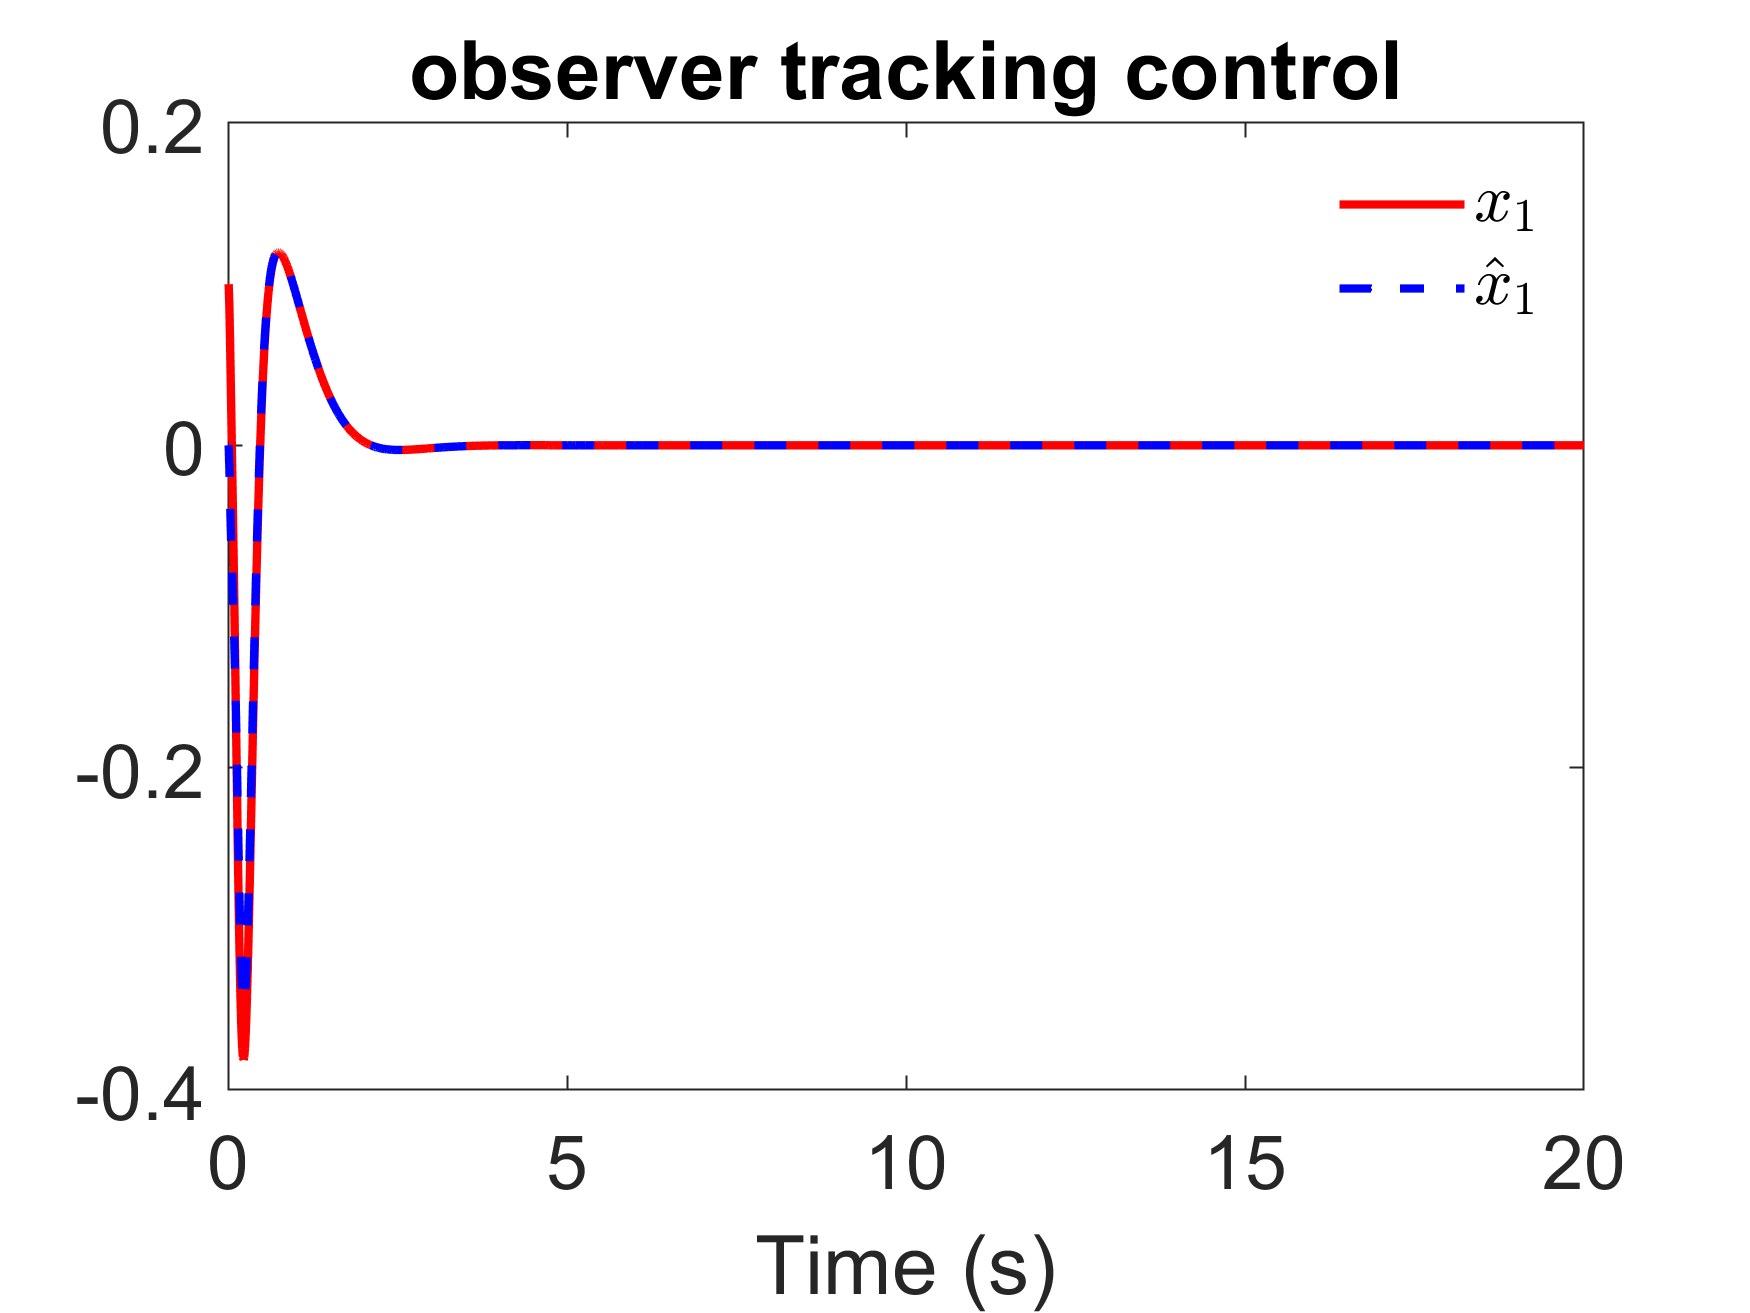
\includegraphics[width=0.6\textwidth]{single_output_observer/fig9.png}
    \caption{Single $y = w$, observer control.}
\end{figure}

\begin{figure}[!ht]
    \centering
    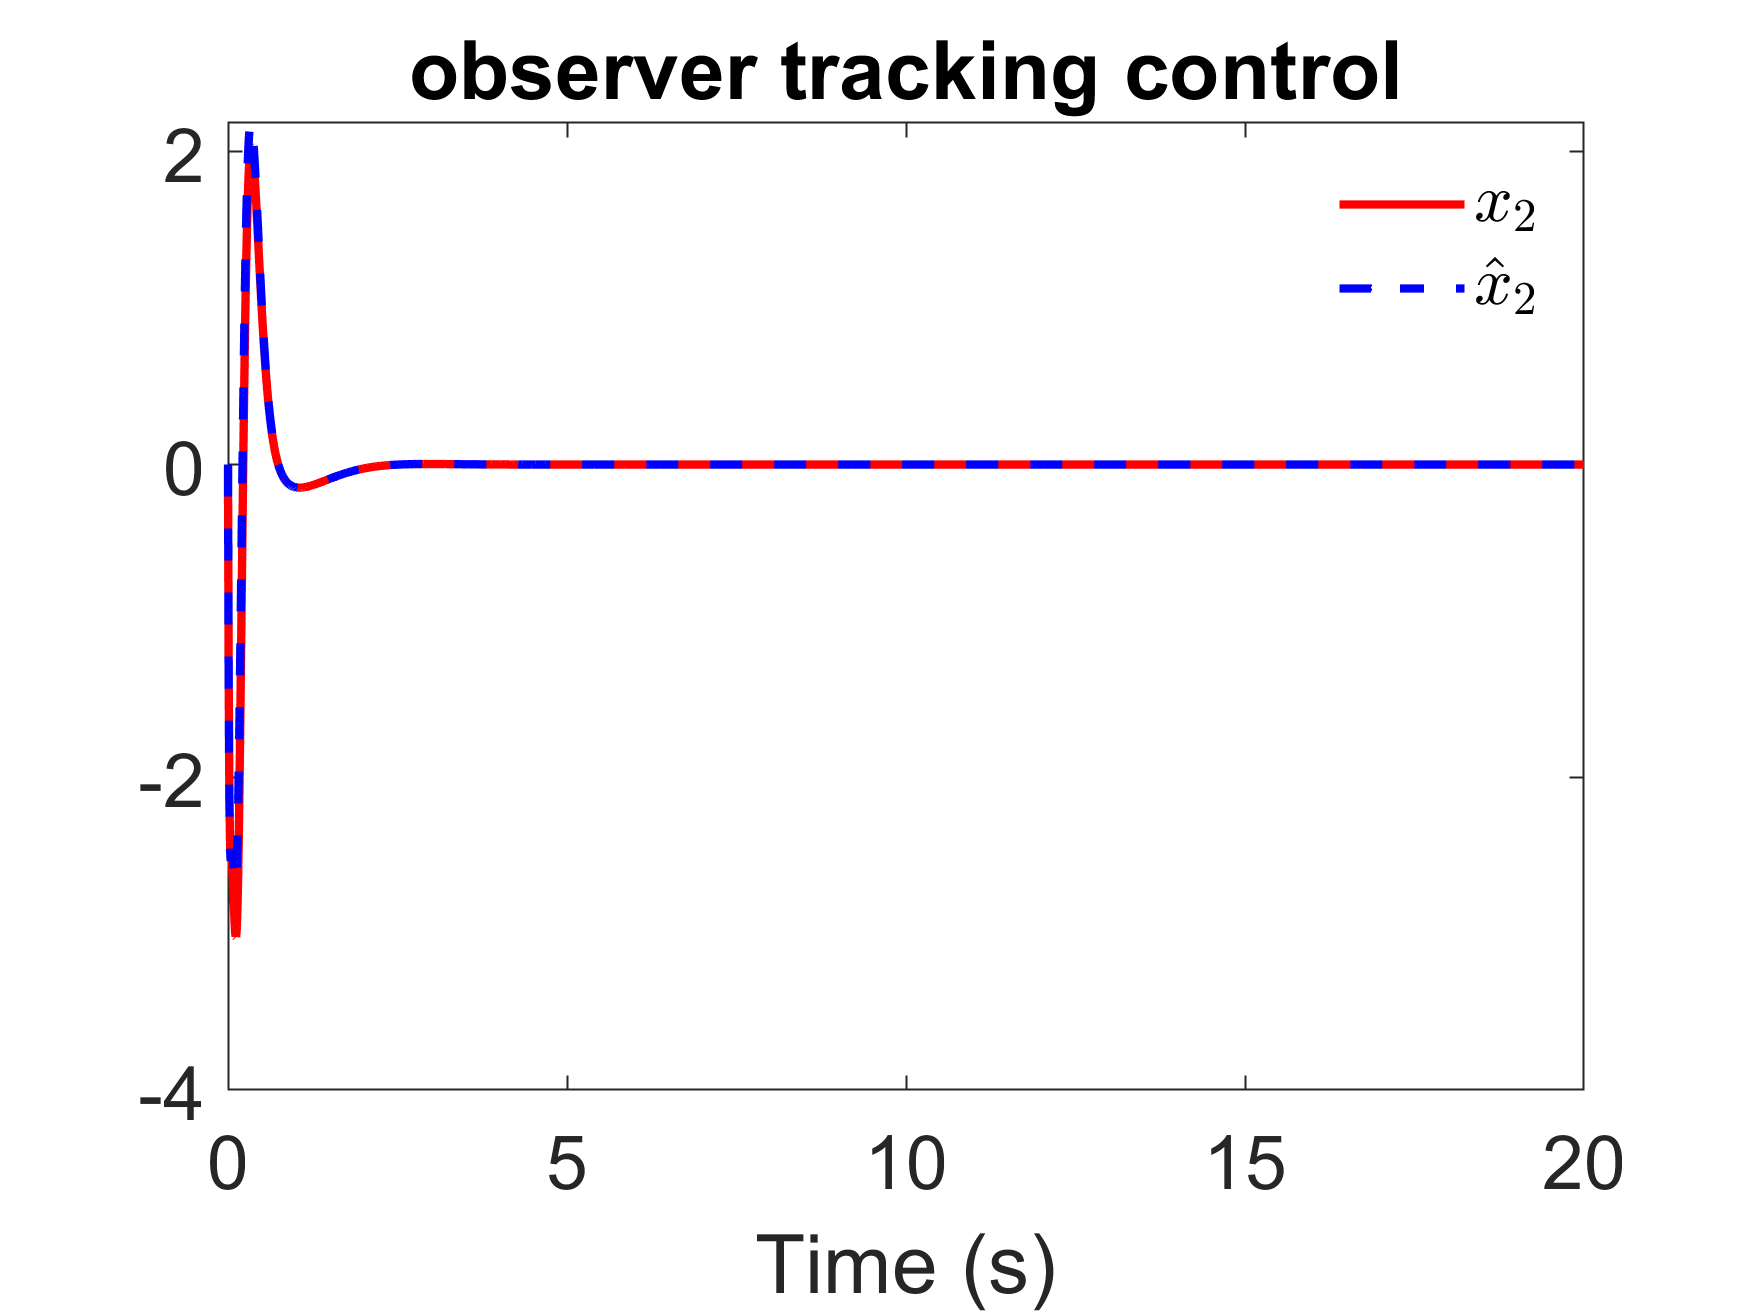
\includegraphics[width=0.6\textwidth]{single_output_observer/fig10.png}
    \caption{Single $y = w$, observer control.}
\end{figure}

\begin{figure}[!ht]
    \centering
    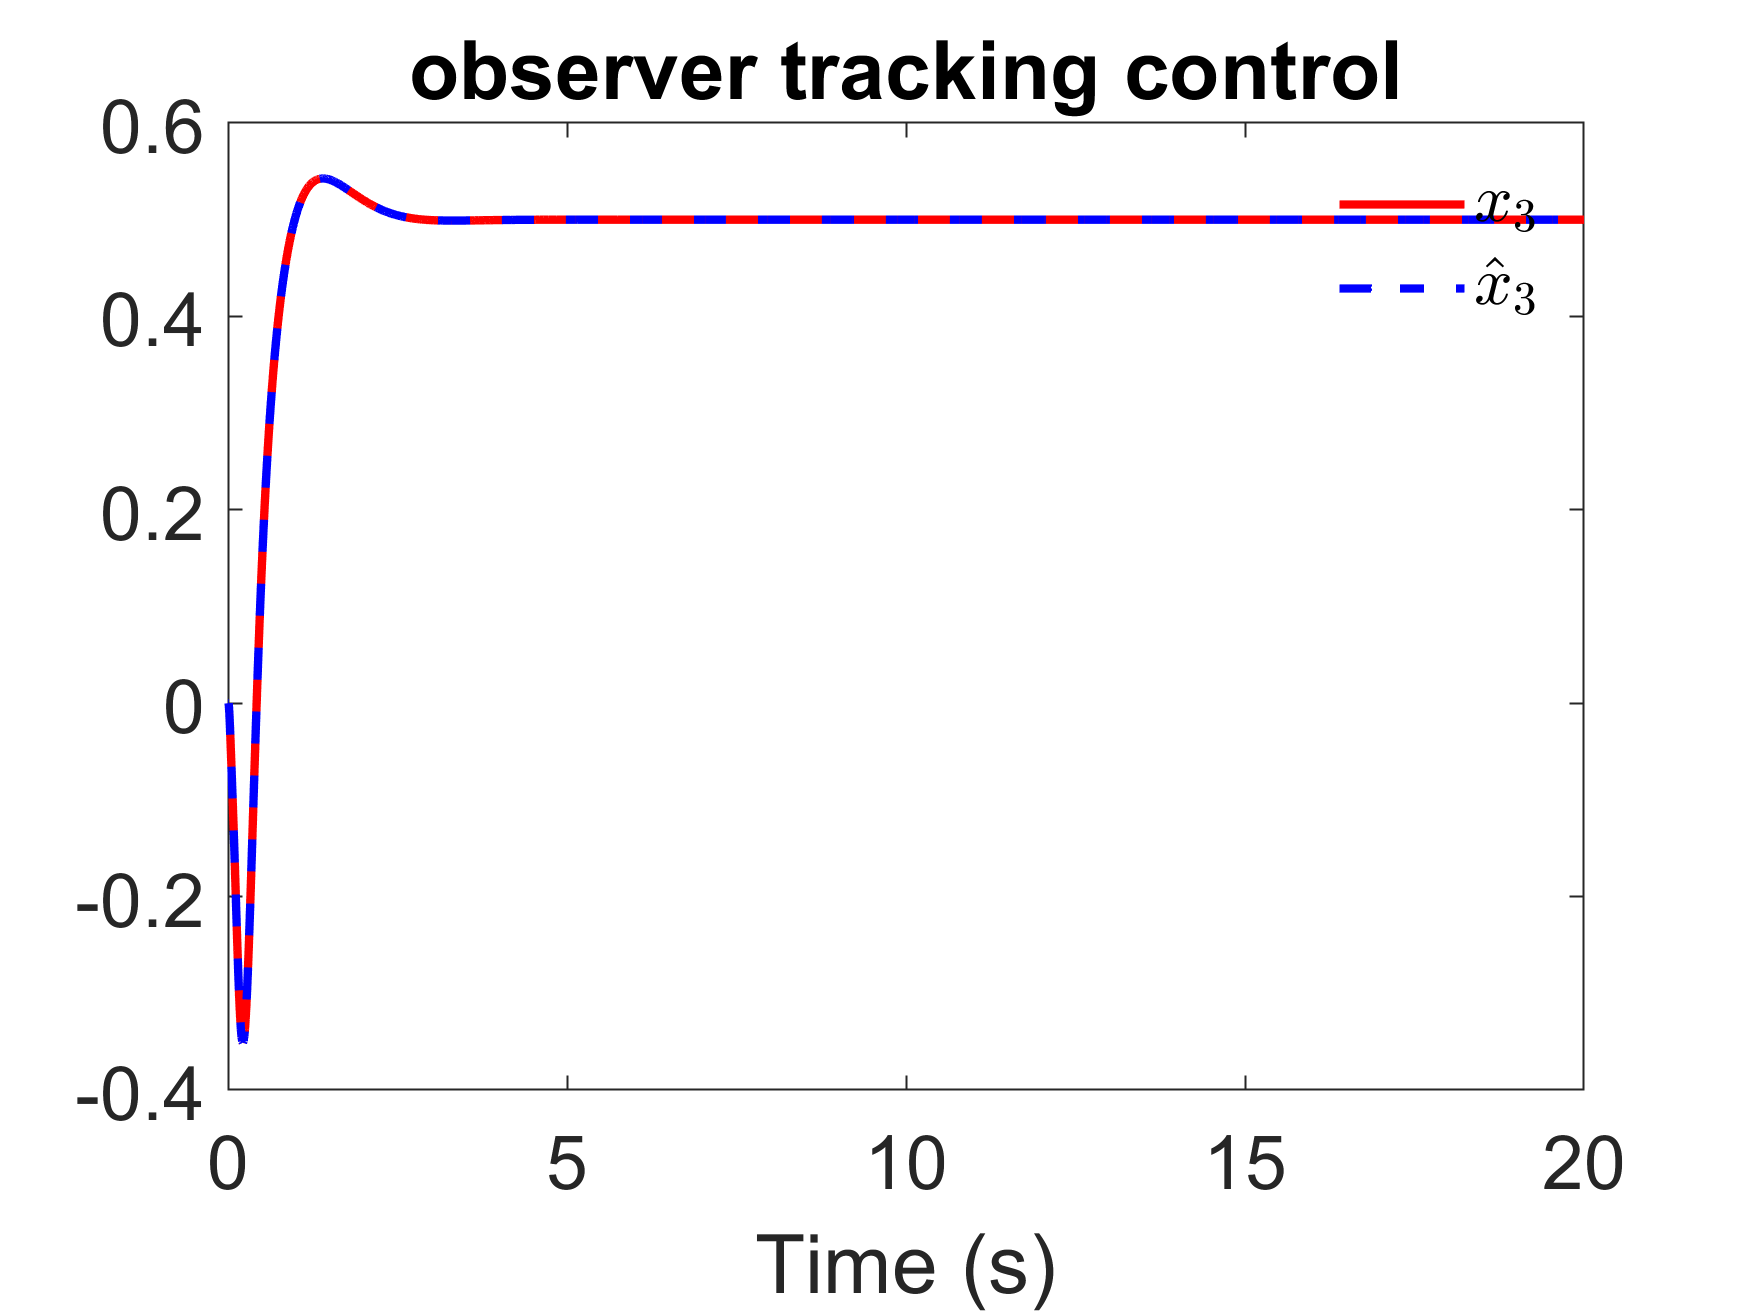
\includegraphics[width=0.6\textwidth]{single_output_observer/fig11.png}
    \caption{Single $y = w$, observer control.}
\end{figure}

\begin{figure}[!ht]
    \centering
    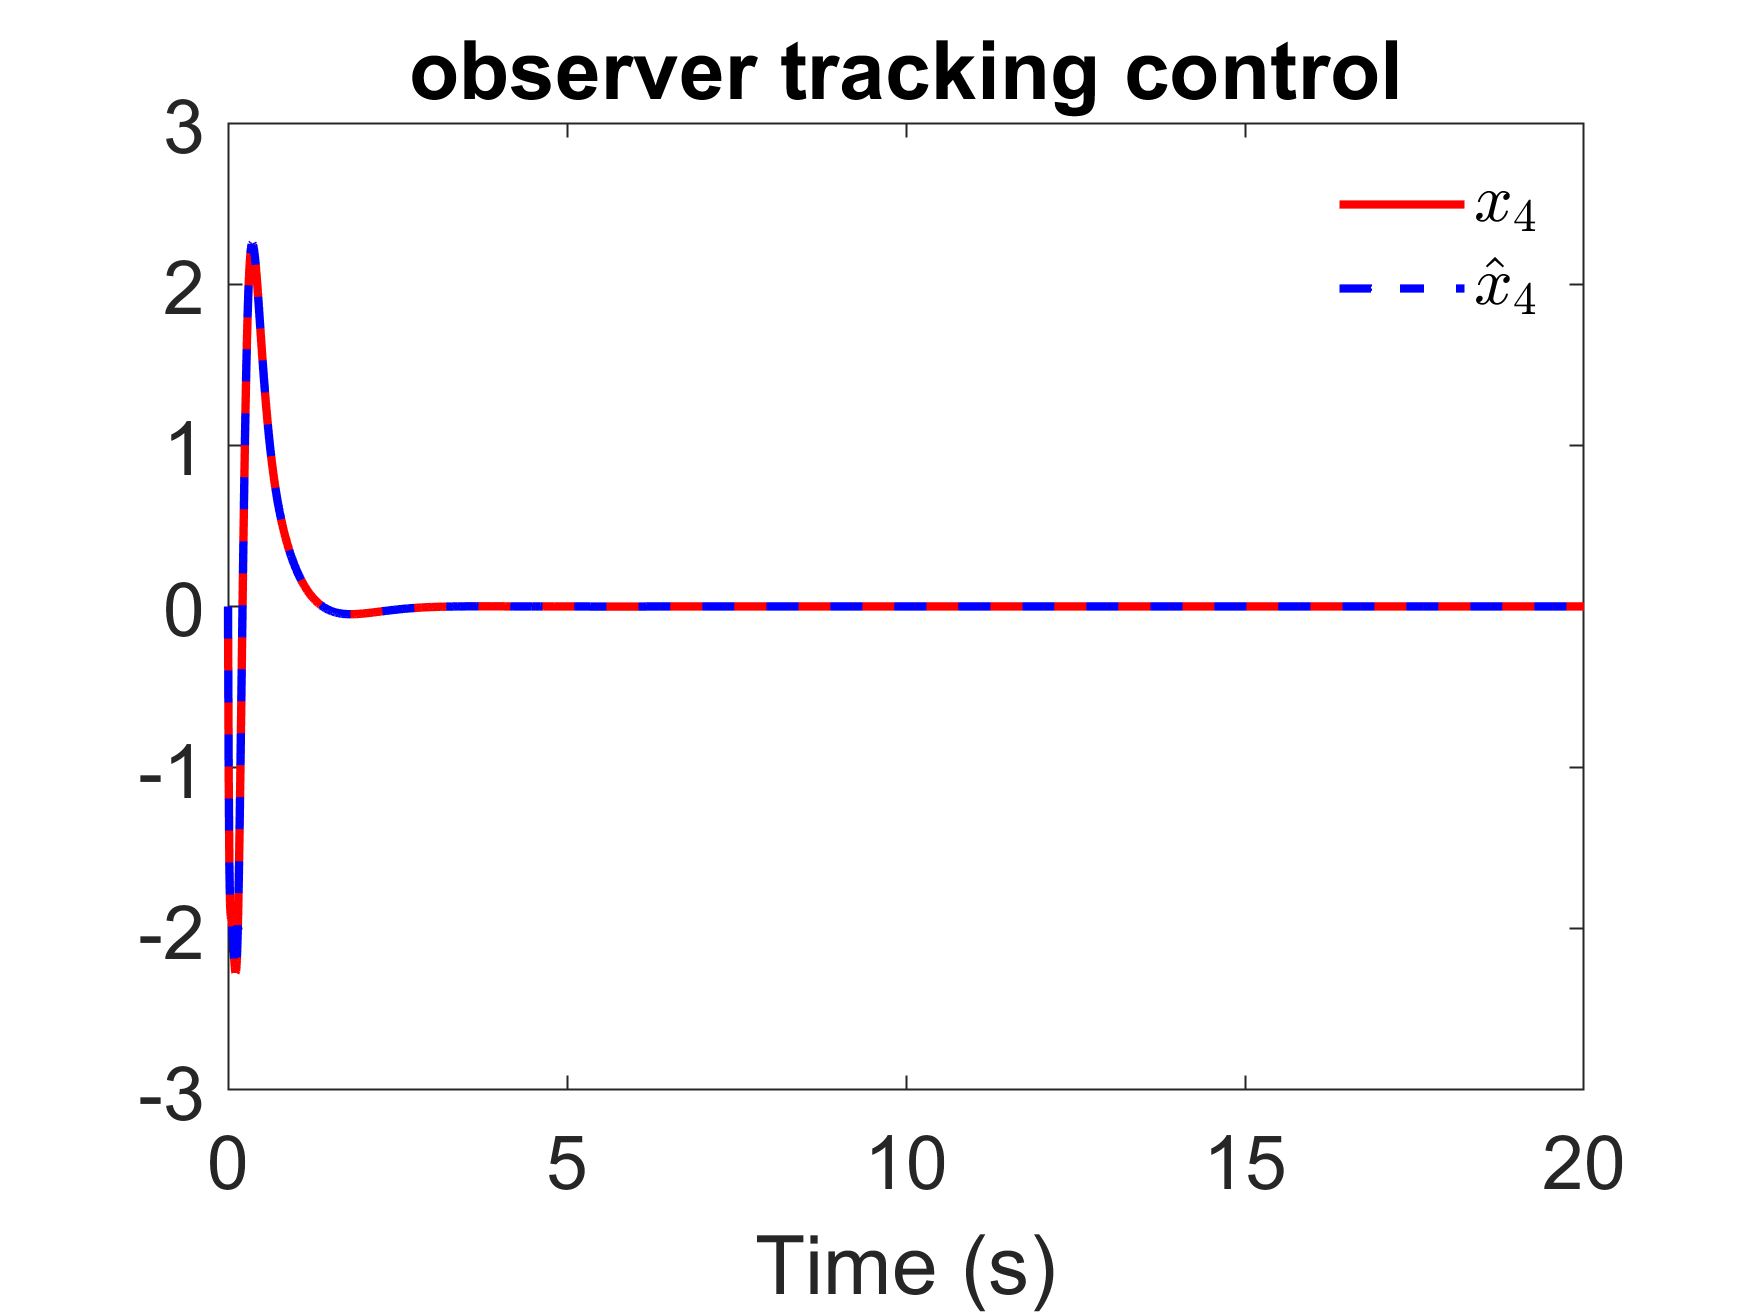
\includegraphics[width=0.6\textwidth]{single_output_observer/fig12.png}
    \caption{Single $y = w$, observer control.}
\end{figure}

\begin{figure}[!ht]
    \centering
    \includegraphics[width=0.6\textwidth]{double_output_observer/fig1.png}
    \caption{Single $y = [\theta,w]^T$, observer control.}
\end{figure}

\begin{figure}[!ht]
    \centering
    \includegraphics[width=0.6\textwidth]{double_output_observer/fig2.png}
    \caption{Single $y = [\theta,w]^T$, observer control.}
\end{figure}

\begin{figure}[!ht]
    \centering
    \includegraphics[width=0.6\textwidth]{double_output_observer/fig3.png}
    \caption{Single $y = [\theta,w]^T$, observer control.}
\end{figure}

\begin{figure}[!ht]
    \centering
    \includegraphics[width=0.6\textwidth]{double_output_observer/fig4.png}
    \caption{Single $y = [\theta,w]^T$, observer control.}
\end{figure}

\begin{figure}[!ht]
    \centering
    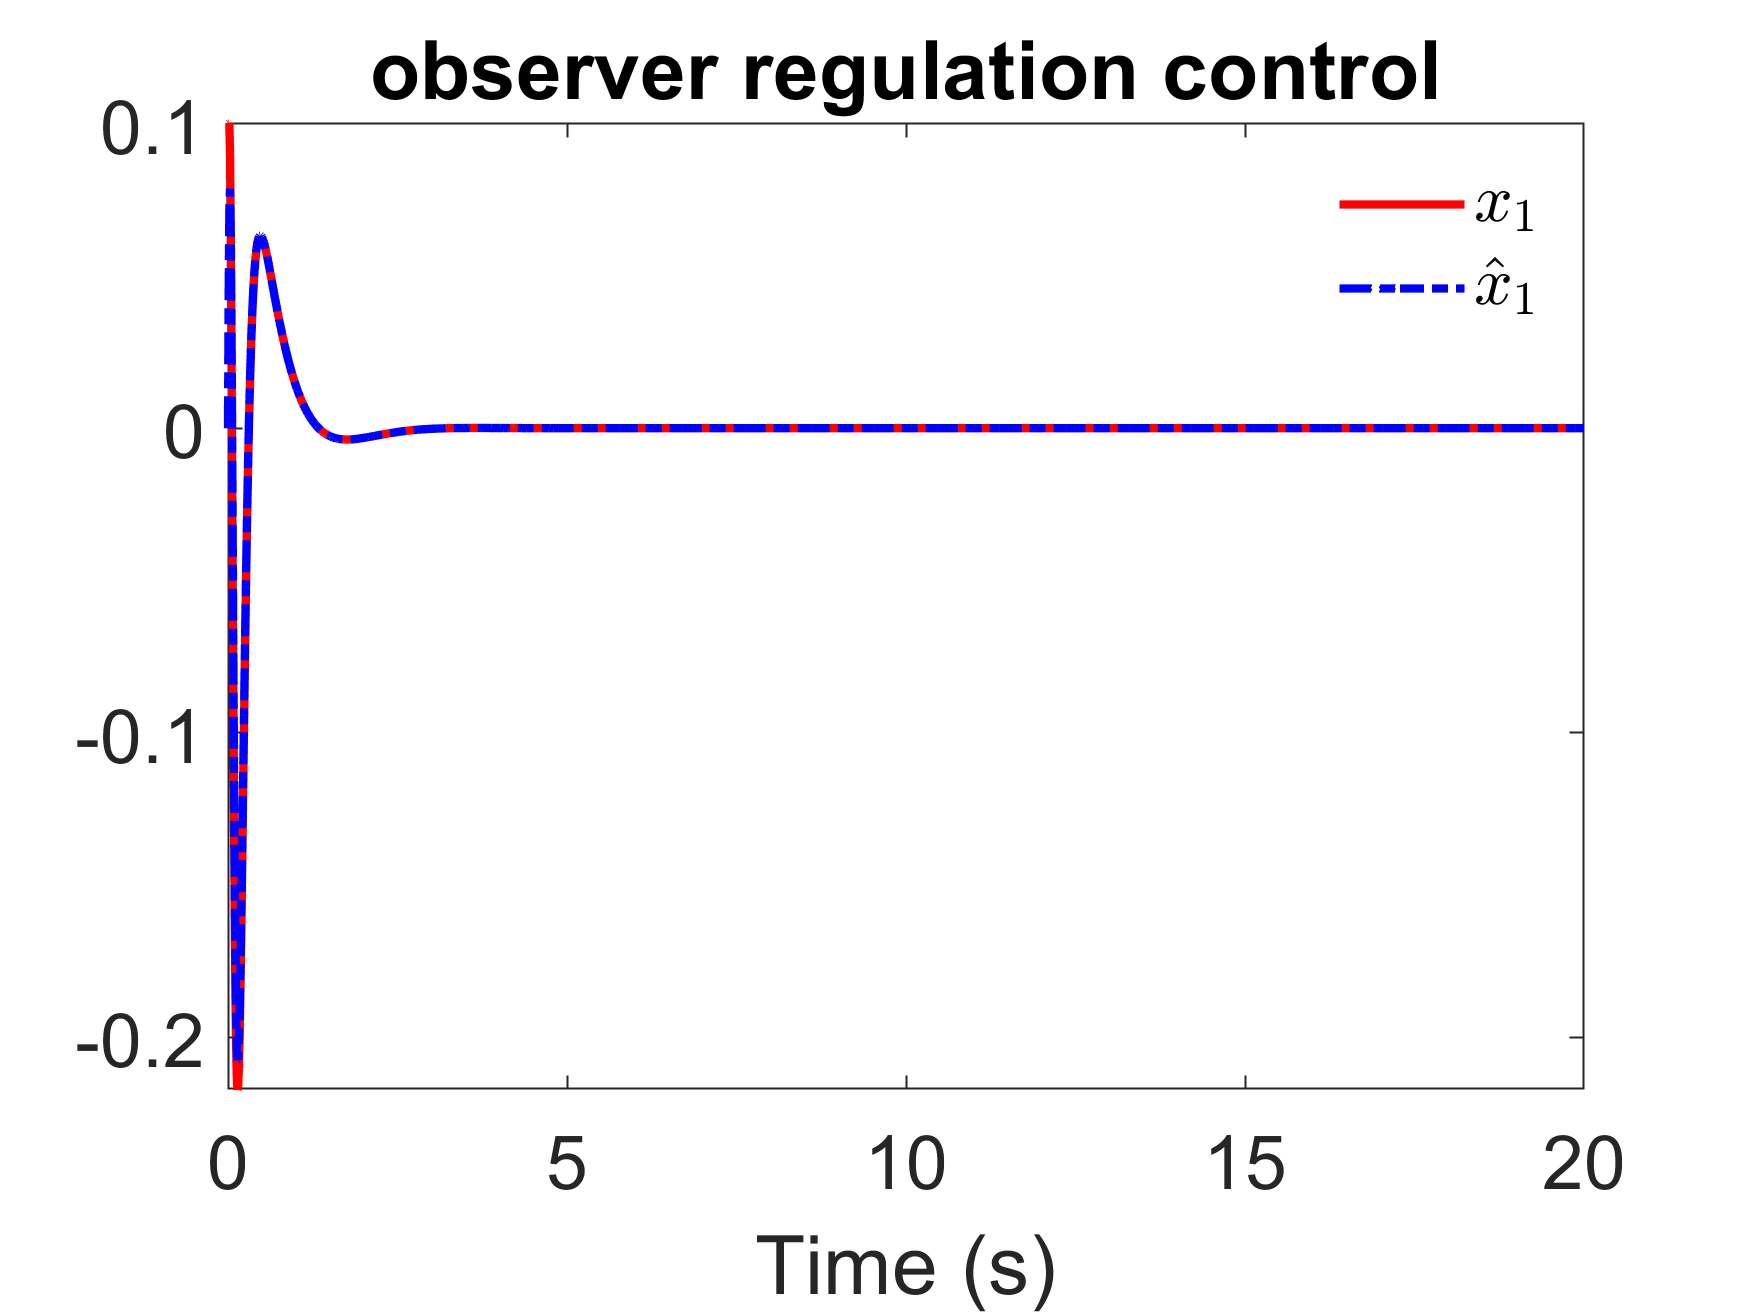
\includegraphics[width=0.6\textwidth]{double_output_observer/fig5.png}
    \caption{Single $y = [\theta,w]^T$, observer control.}
\end{figure}

\begin{figure}[!ht]
    \centering
    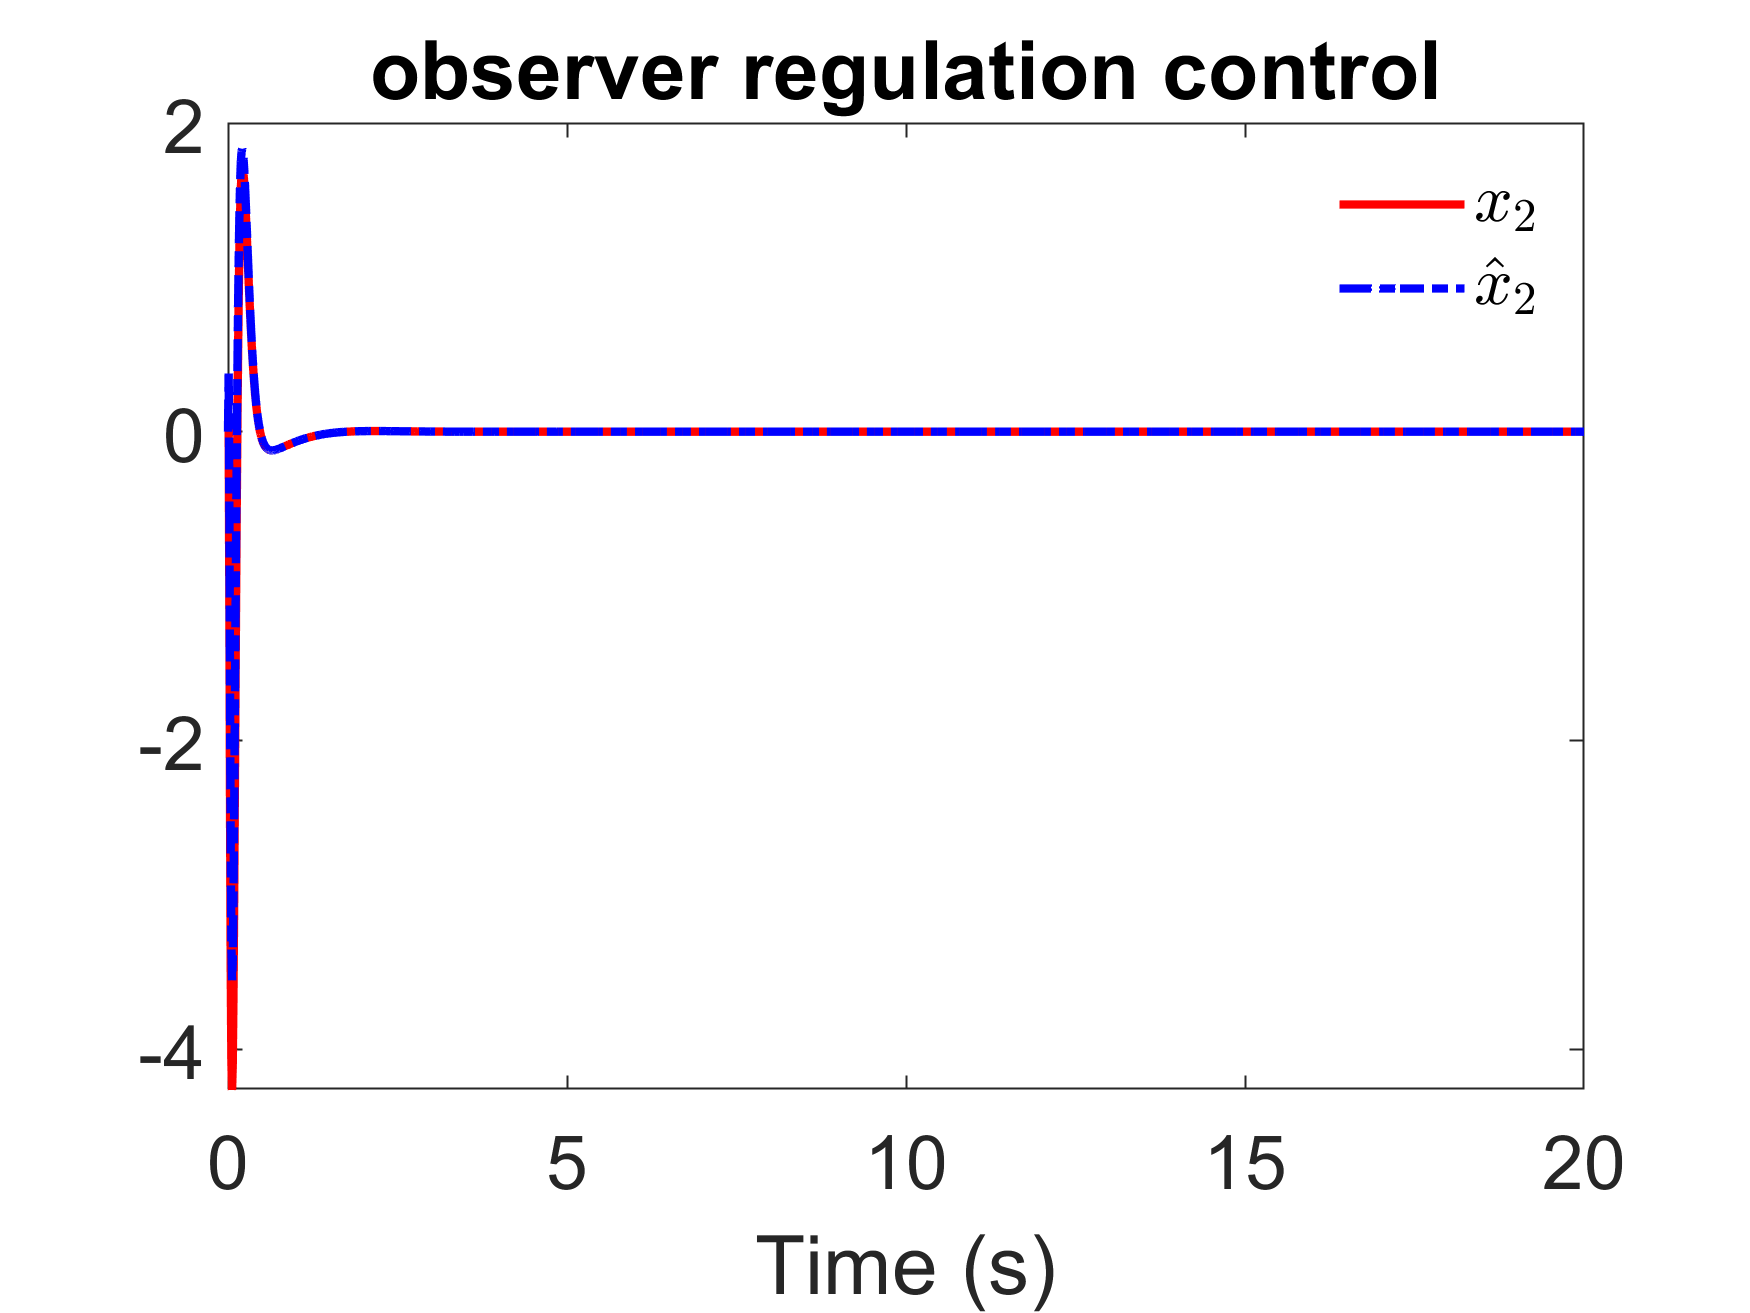
\includegraphics[width=0.6\textwidth]{double_output_observer/fig6.png}
    \caption{Single $y = [\theta,w]^T$, observer control.}
\end{figure}

\begin{figure}[!ht]
    \centering
    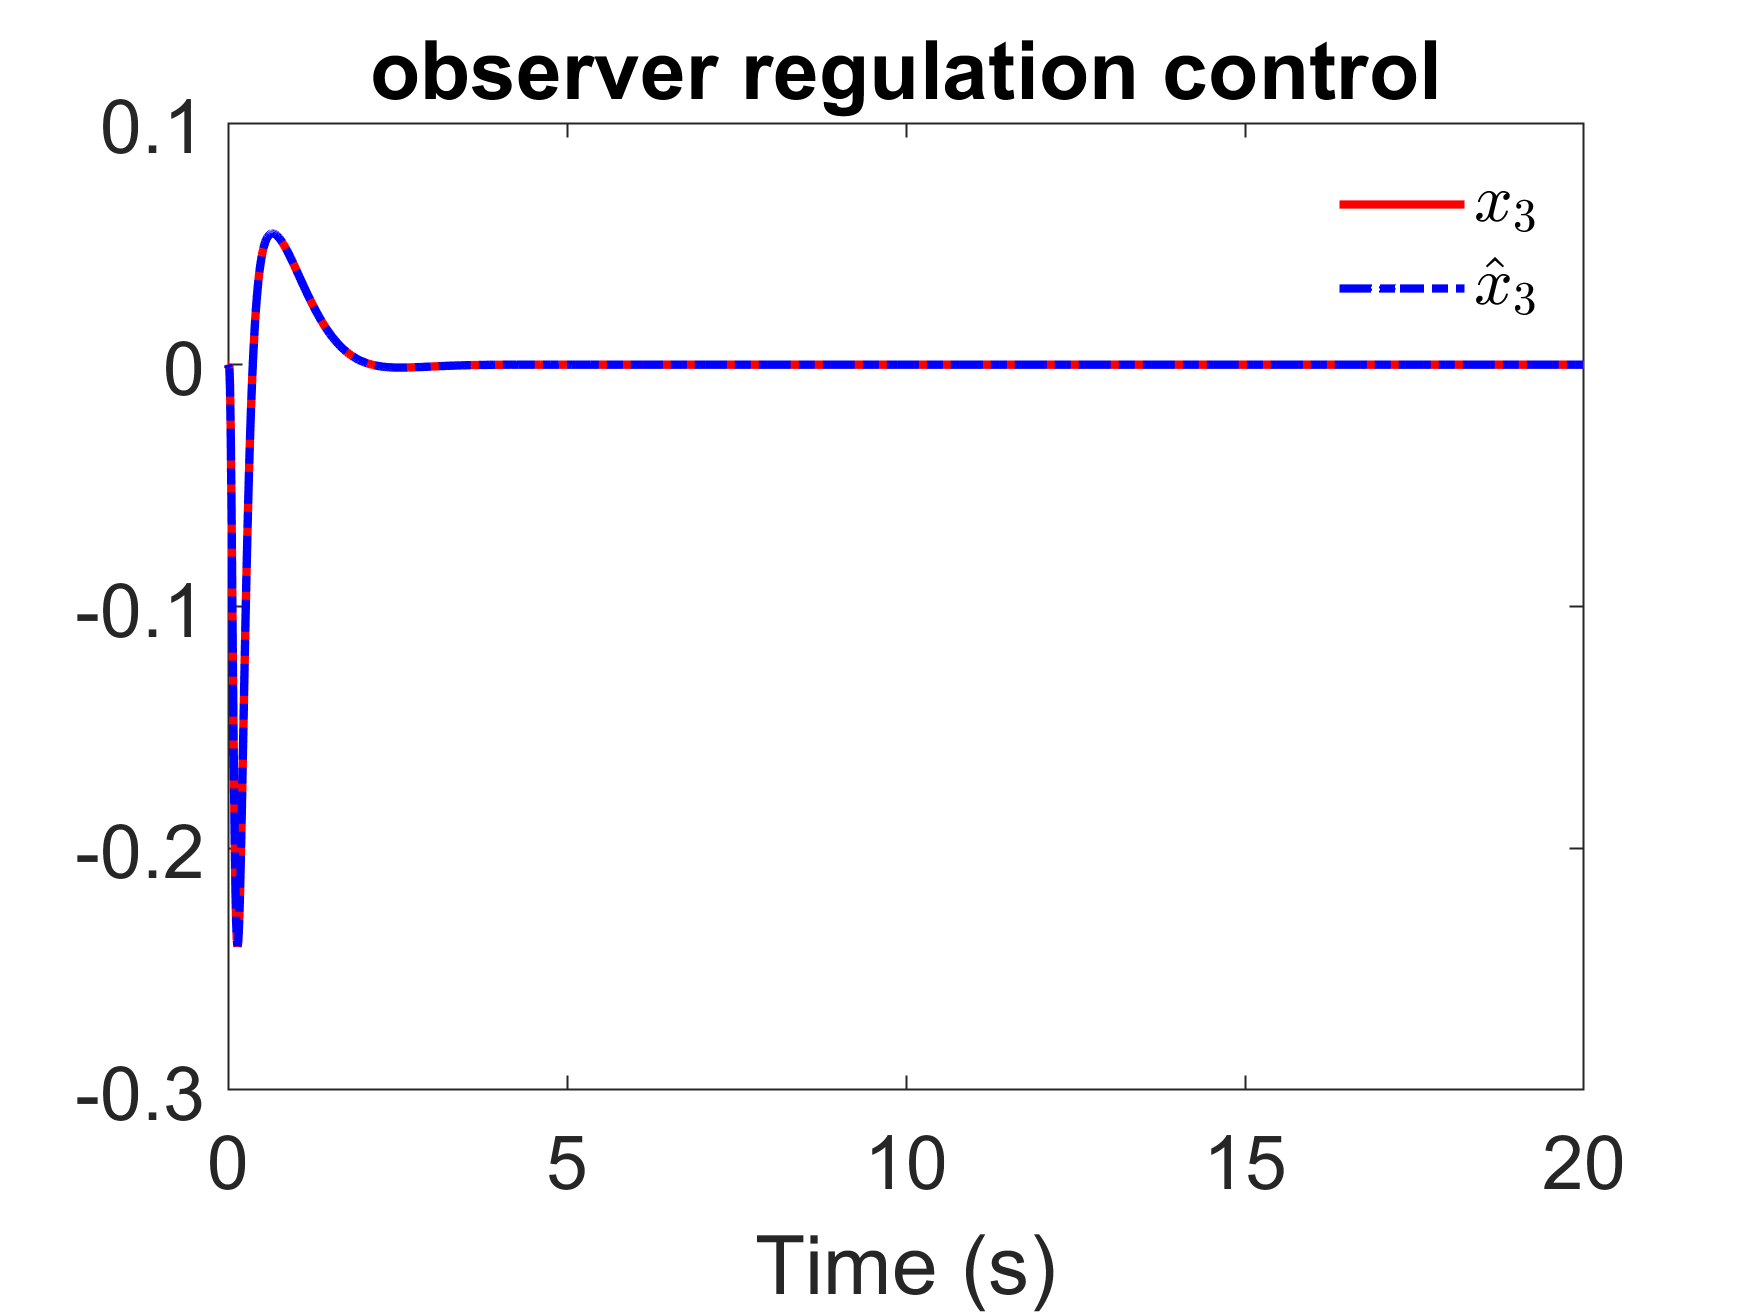
\includegraphics[width=0.6\textwidth]{double_output_observer/fig7.png}
    \caption{Single $y = [\theta,w]^T$, observer control.}
\end{figure}

\begin{figure}[!ht]
    \centering
    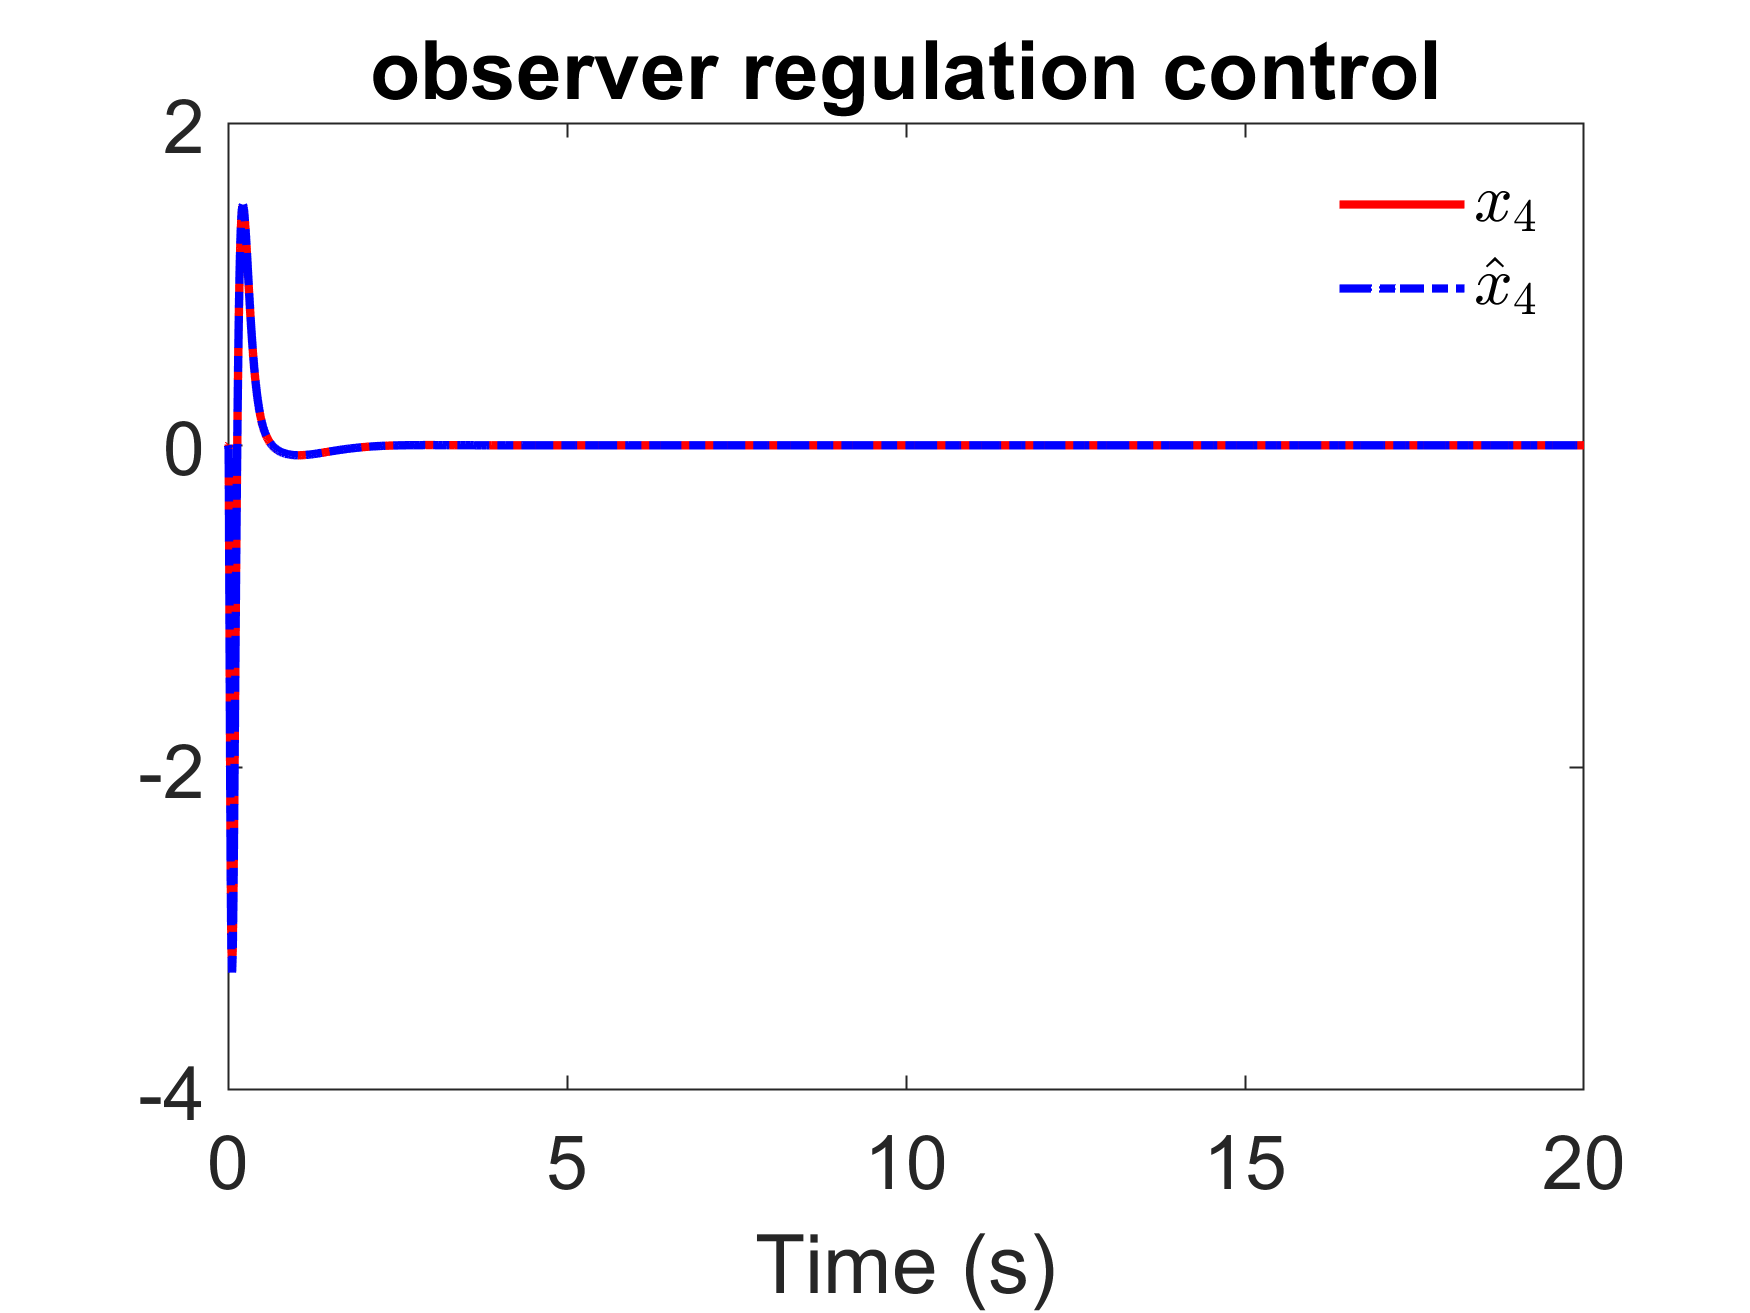
\includegraphics[width=0.6\textwidth]{double_output_observer/fig8.png}
    \caption{Single $y = [\theta,w]^T$, observer control.}
\end{figure}

\begin{figure}[!ht]
    \centering
    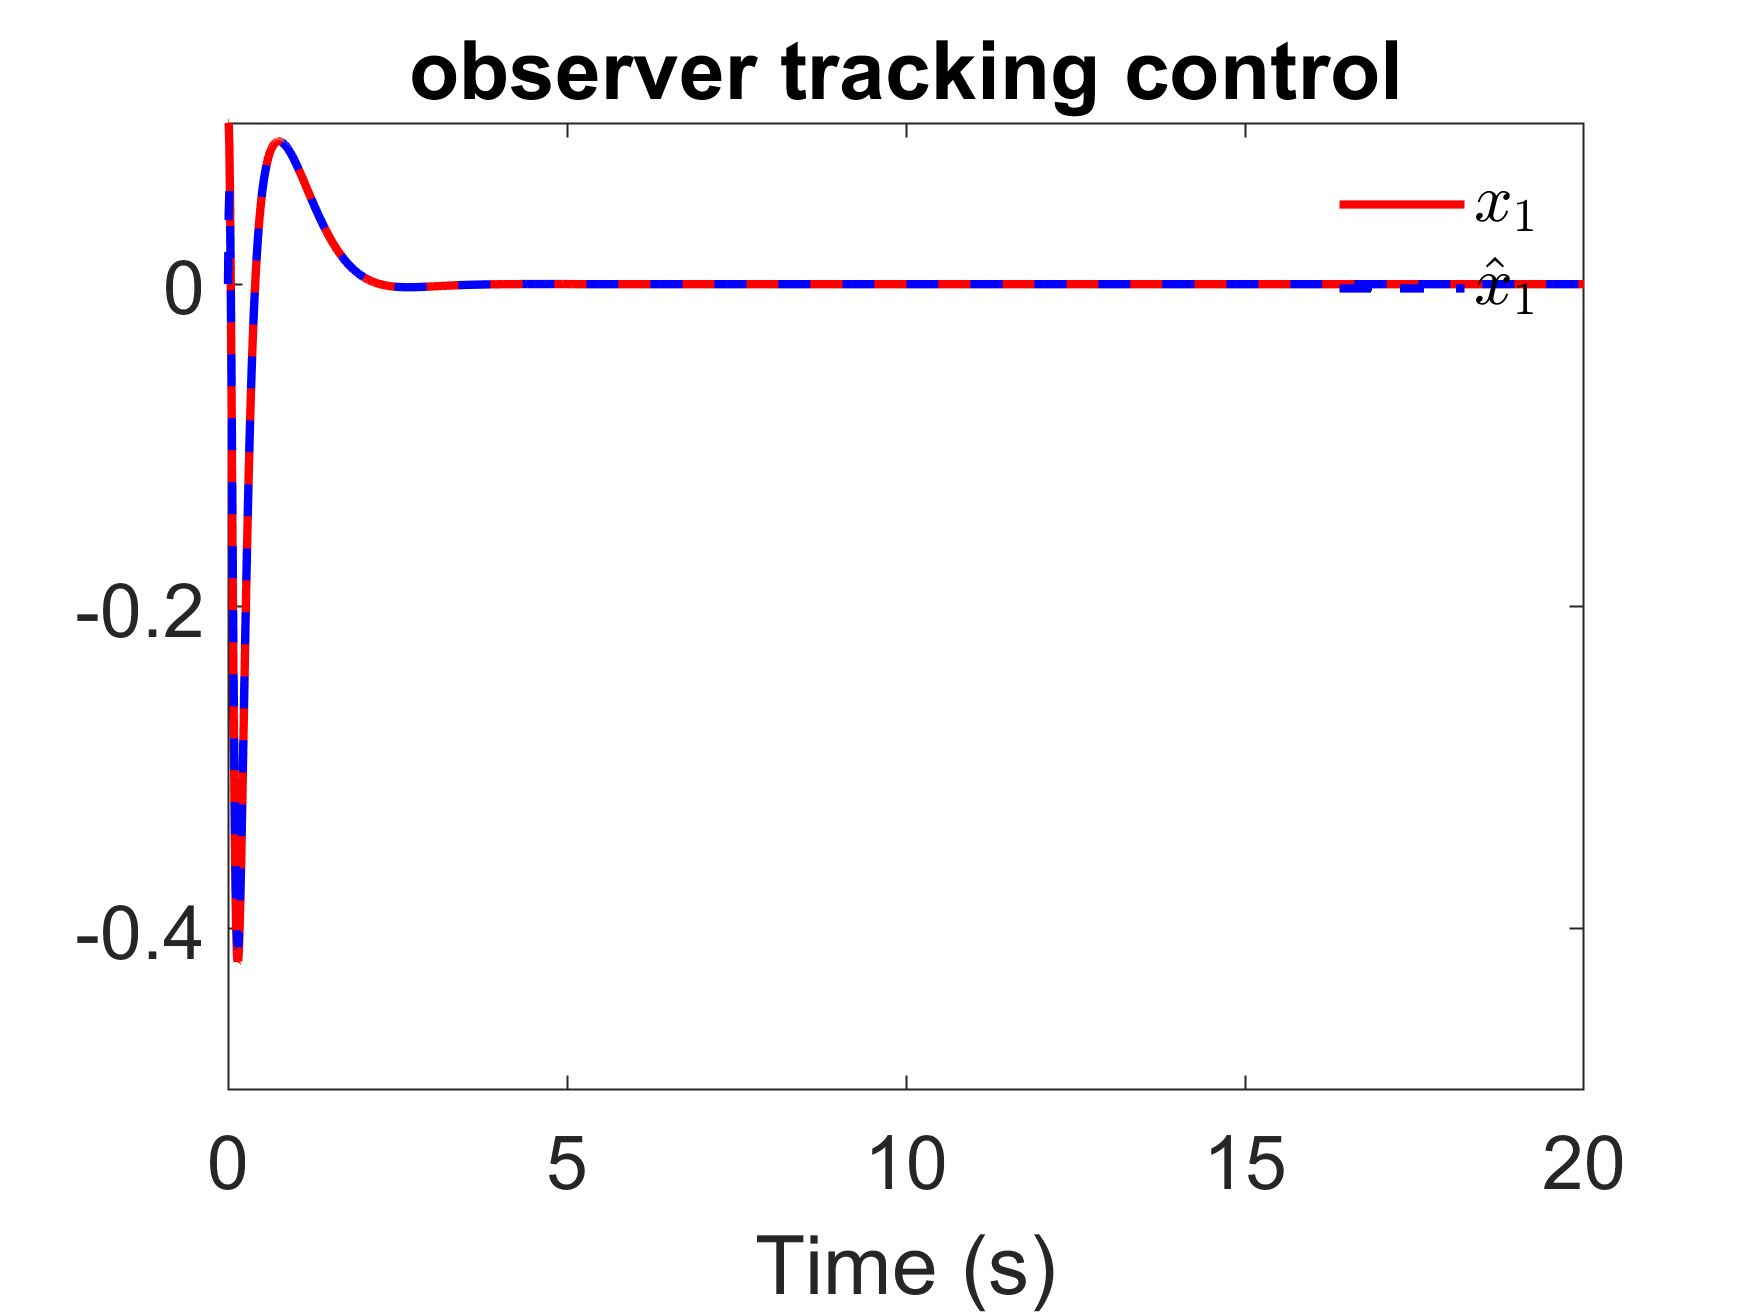
\includegraphics[width=0.6\textwidth]{double_output_observer/fig9.png}
    \caption{Single $y = [\theta,w]^T$, observer control.}
\end{figure}

\begin{figure}[!ht]
    \centering
    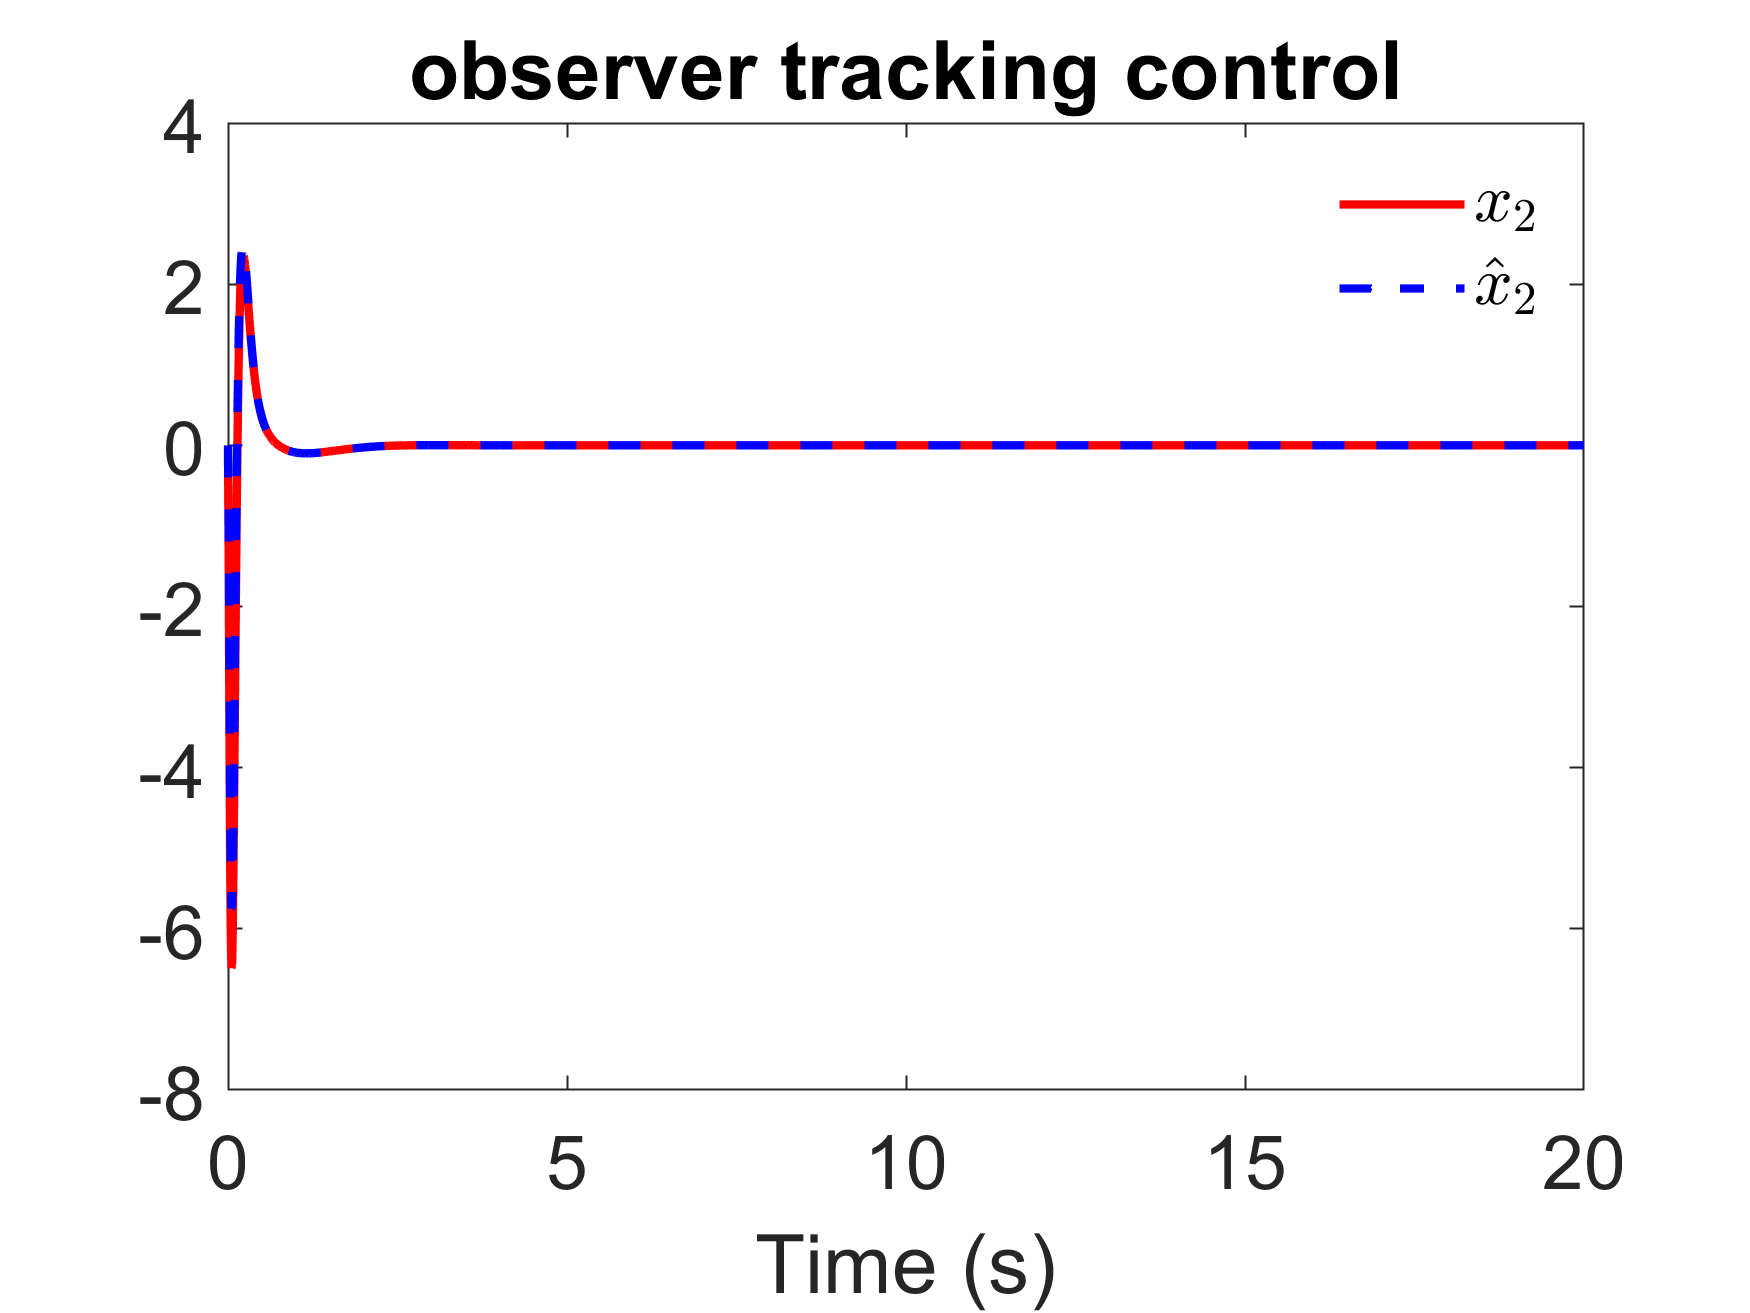
\includegraphics[width=0.6\textwidth]{double_output_observer/fig10.png}
    \caption{Single $y = [\theta,w]^T$, observer control.}
\end{figure}

\begin{figure}[!ht]
    \centering
    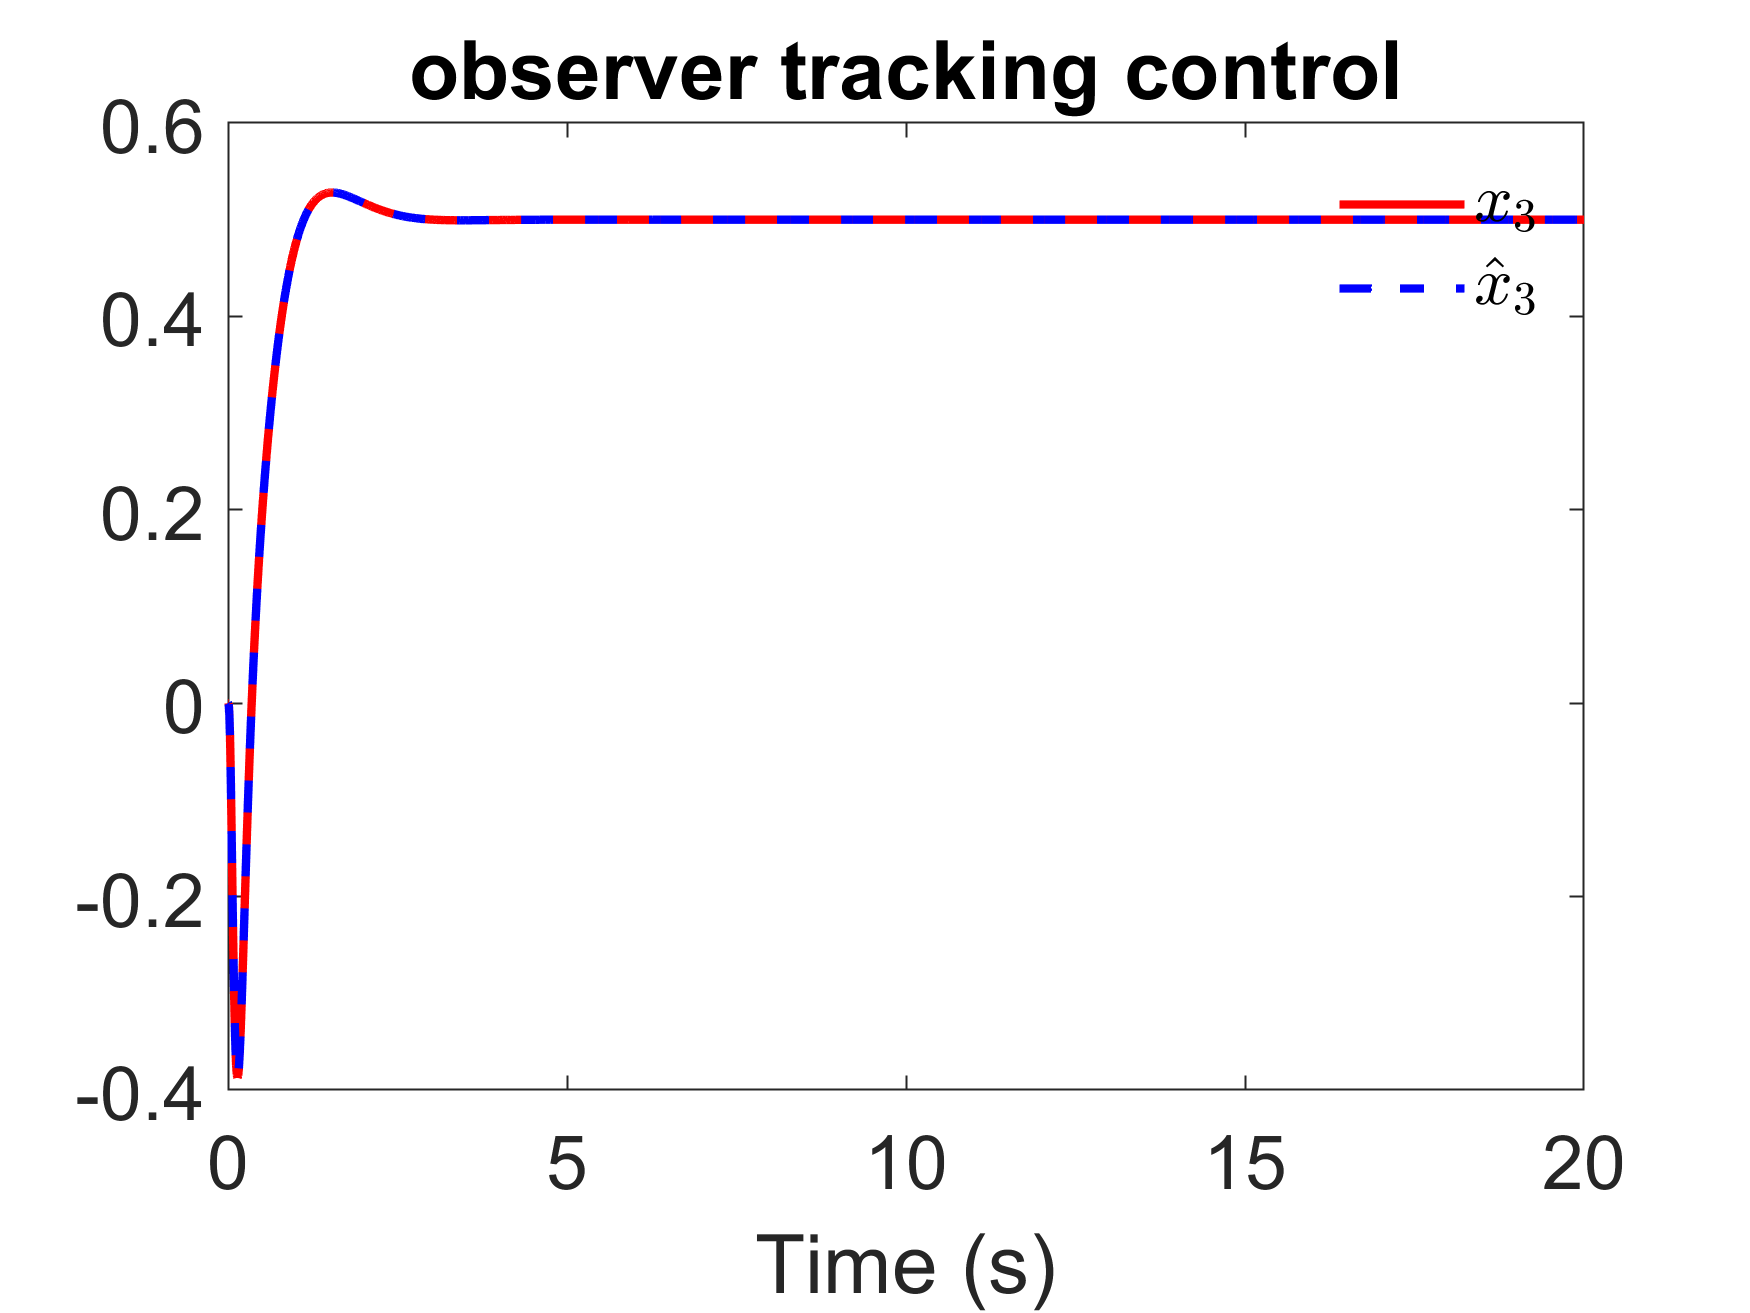
\includegraphics[width=0.6\textwidth]{double_output_observer/fig11.png}
    \caption{Single $y = [\theta,w]^T$, observer control.}
\end{figure}

\begin{figure}[!ht]
    \centering
    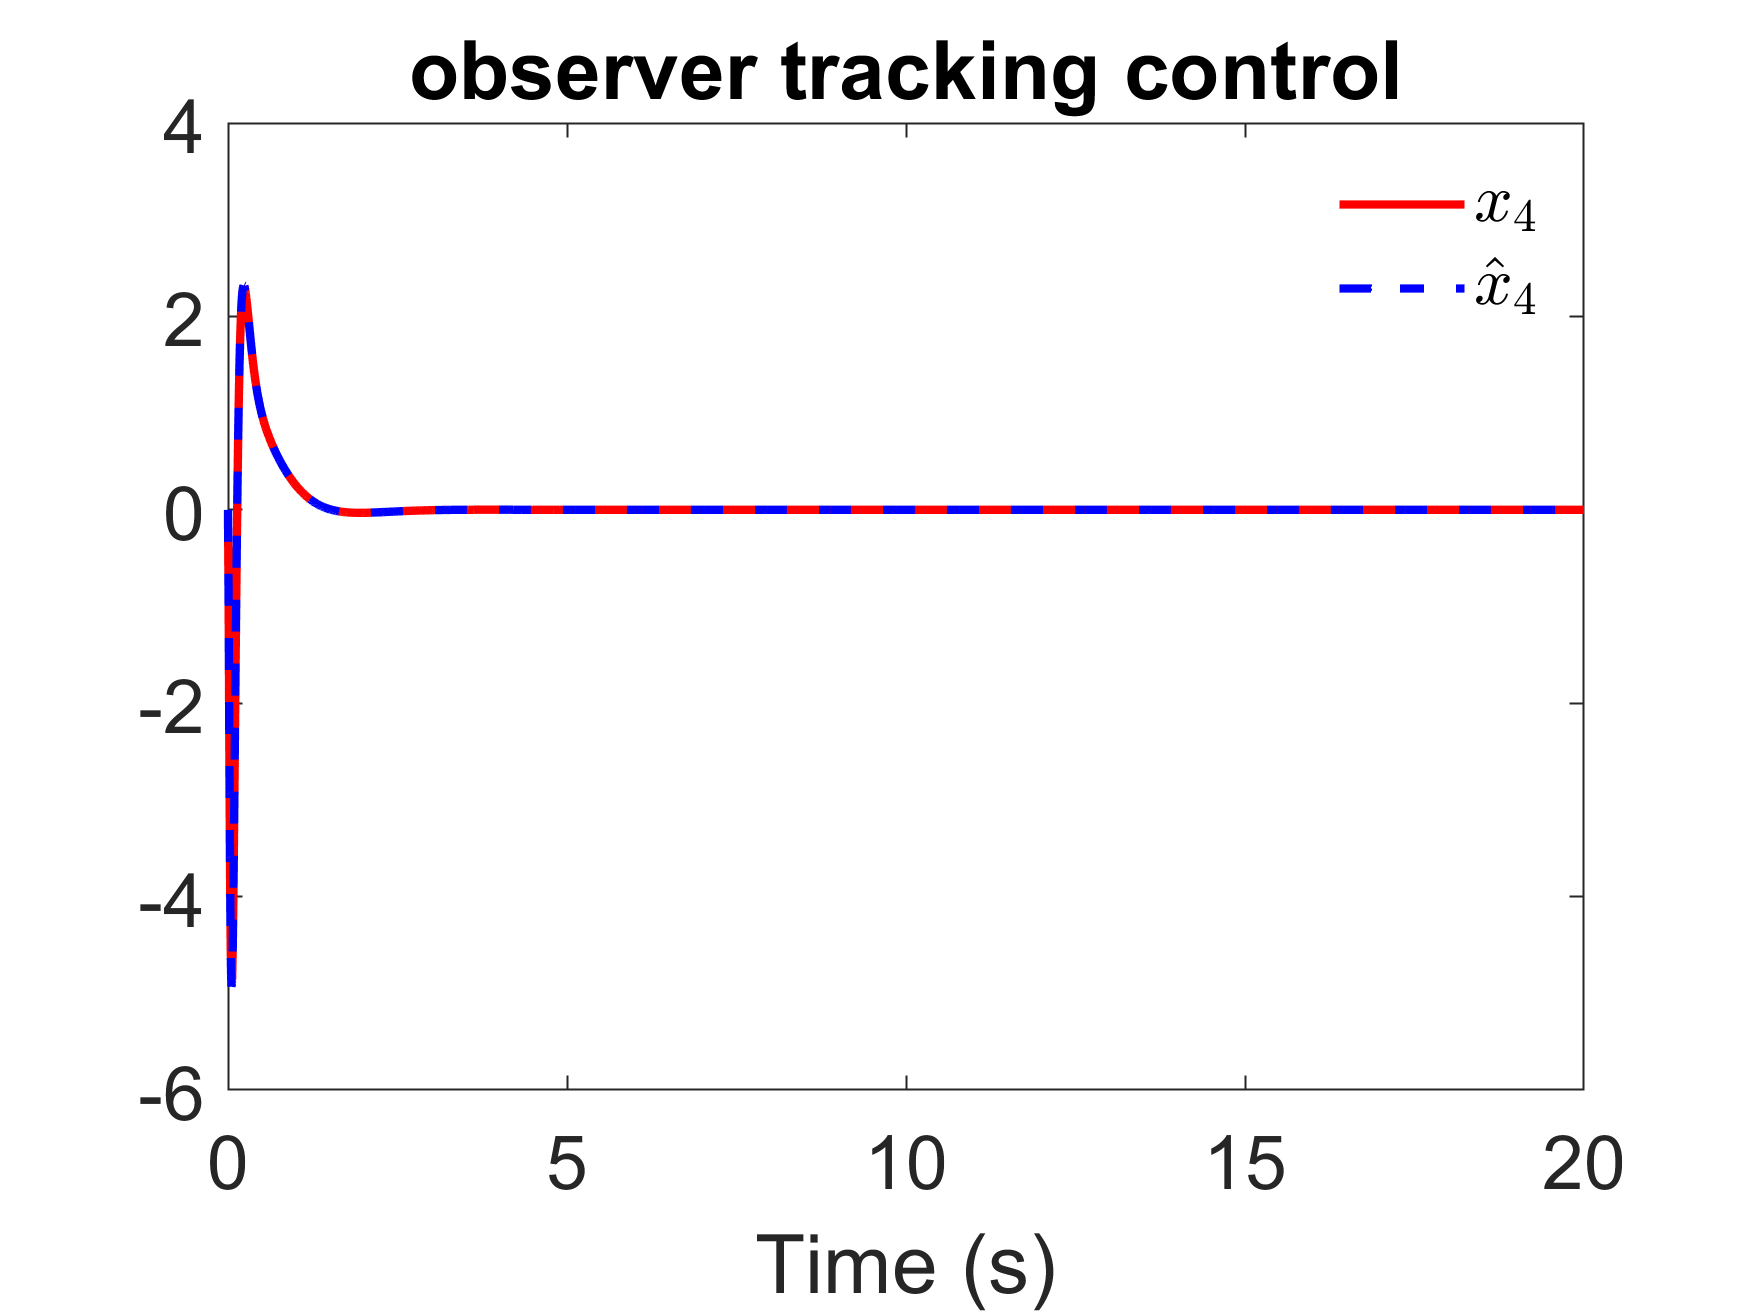
\includegraphics[width=0.6\textwidth]{double_output_observer/fig12.png}
    \caption{Single $y = [\theta,w]^T$, observer control.}
    \label{fig:observer_sim_last}
\end{figure}

\begin{figure}
    \centering
    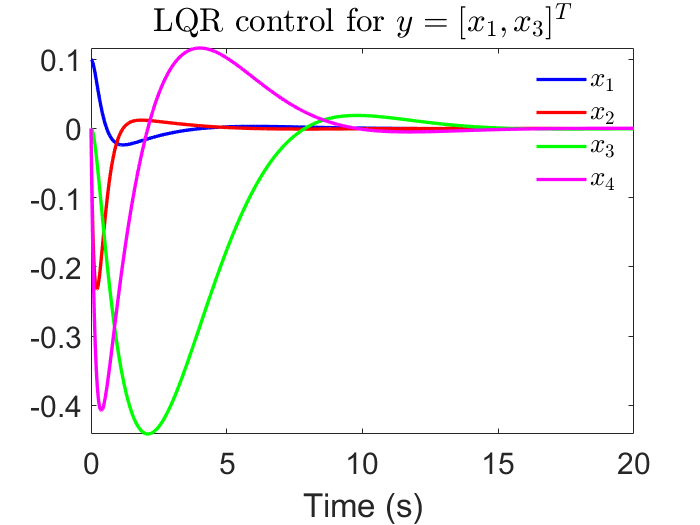
\includegraphics[width=0.6\textwidth]{lqr/lqr_1.png}
    \caption{LQR state feedback results for $y = [x_1, x_3]^T$.}
    \label{fig:lqr1}
\end{figure}

\begin{figure}
    \centering
    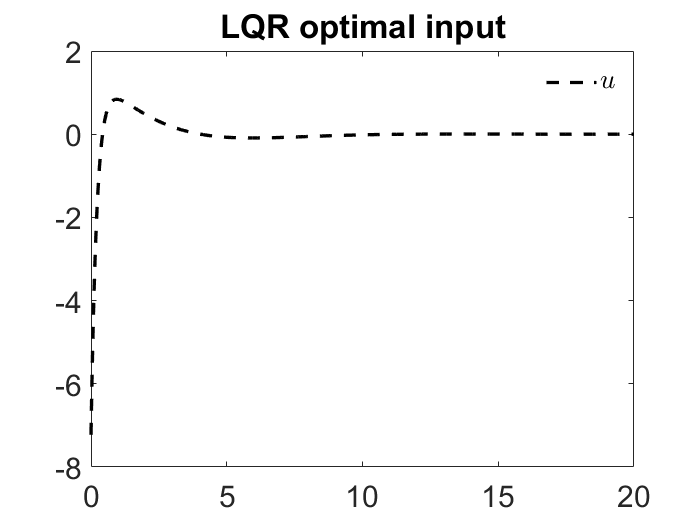
\includegraphics[width=0.6\textwidth]{lqr/lqr_2.png}
    \caption{LQR input for $y = [x_1, x_3]^T$.}
    \label{fig:lqr2}
\end{figure}

\begin{figure}
    \centering
    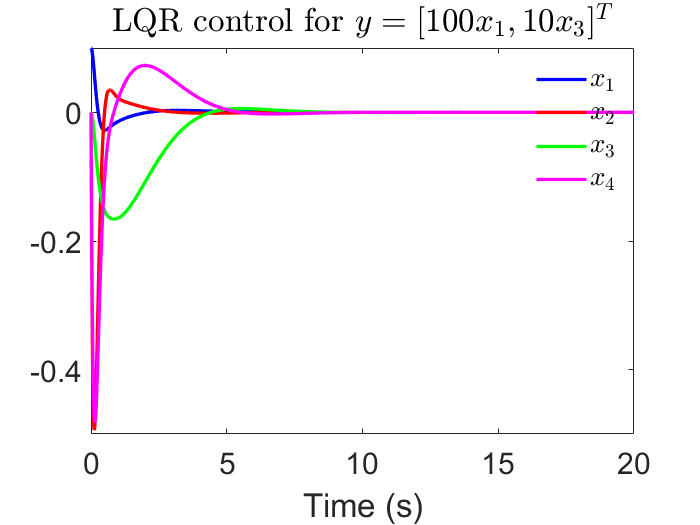
\includegraphics[width=0.6\textwidth]{lqr/lqr_3.png}
    \caption{LQR state feedback results for $y = [100 x_1, 10 x_3]^T$.}
    \label{fig:lqr3}
\end{figure}

\begin{figure}
    \centering
    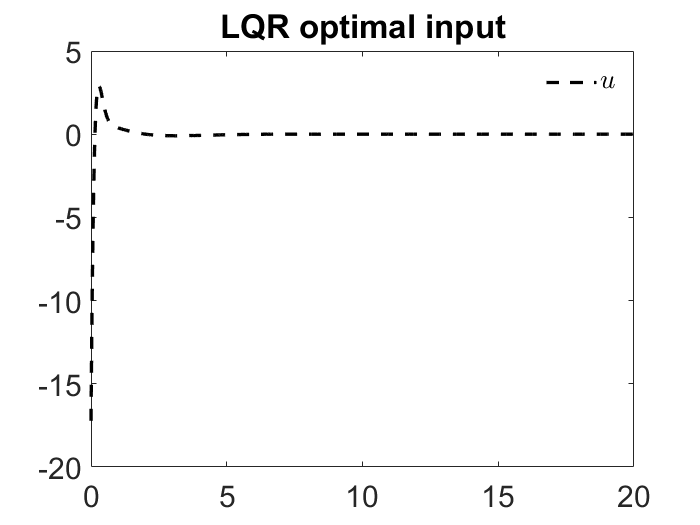
\includegraphics[width=0.6\textwidth]{lqr/lqr_4.png}
    \caption{LQR optimal input for $y = [100 x_1, 10 x_3]^T$.}
    \label{fig:lqr4}
\end{figure}

\begin{figure}
    \centering
    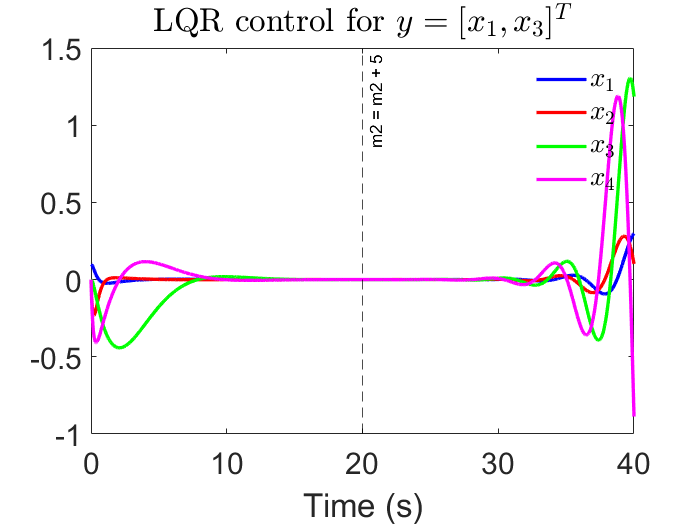
\includegraphics[width=0.6\textwidth]{lqr_offset_m2_5kg.png}
    \caption{LQR results for pendulum mass perturbation by $\delta m_2 = 5$kg at $t = 20$s.}
    \label{fig:lqr_perturb_5kg}
\end{figure}

\begin{figure}
    \centering
    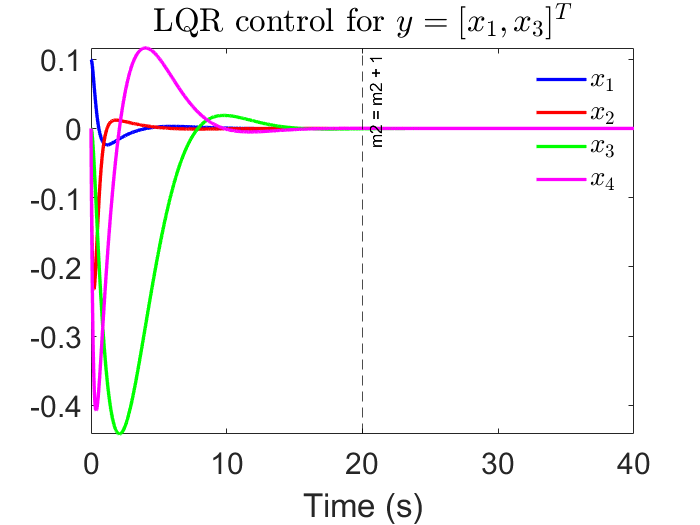
\includegraphics[width=0.6\textwidth]{lqr_offset_m2_1kg.png}
    \caption{LQR results for pendulum mass perturbation by $\delta m_2 = 1$kg at $t = 20$s.}
    \label{fig:lqr_perturb_1kg}
\end{figure}


\end{document}

